%% =====================================================================
%% TFI - CAMPOS - SCARAZZINI
%% Documento unificado: preámbulo, portada, frontmatter, capítulos y anexos
%% en un único archivo .tex.
%%
%% Mapa del documento (buscar los banners "%% ====" para navegar):
%%   1. PREÁMBULO            (antes preambulo.tex)
%%   2. PORTADA              (antes portada.tex)
%%   3. RESUMEN              (antes frontmatter/resumen.tex)
%%   4. AGRADECIMIENTOS      (antes frontmatter/agradecimientos.tex)
%%   5. INTRODUCCIÓN         (antes capitulos/introduccion.tex)
%%   6. MARCO TEÓRICO        (antes capitulos/marco_teorico.tex)
%%   7. DESARROLLO DEL PRODUCTO (antes capitulos/desarrollo_producto.tex)
%%   8. RESULTADOS           (antes capitulos/resultados.tex)
%%   9. BIBLIOGRAFÍA
%%  10. ANEXOS               (antes capitulos/anexos.tex)
%%  11. LISTADO DE SÍMBOLOS  (antes capitulos/simbolos.tex)
%% =====================================================================

\documentclass[12pt,twoside,a4paper]{report}


%% =====================================================================
%% 1. PREÁMBULO
%% =====================================================================

% ============================================================
% Preámbulo - Tesis UNC / FCEFyN - Escuela de Ingeniería Industrial
% ============================================================

% --- Idioma y codificación ---
\usepackage[utf8]{inputenc}
\usepackage[T1]{fontenc}
\usepackage{lmodern}                 % [A1] fuente Type-1 con mapa Unicode
\input{glyphtounicode}
\pdfgentounicode=1                   % [A1] arregla copiado de ligaduras fi/fl
\usepackage[spanish,es-noquoting]{babel}
\spanishdecimal{,}
\usepackage{microtype}

% --- Página y espaciado ---
\usepackage[a4paper,left=3cm,right=2.5cm,top=2.5cm,bottom=2.5cm]{geometry}
\usepackage{setspace}
\doublespacing

% --- Tablas, figuras, matemática ---
\usepackage{graphicx}
\usepackage{calc}
\usepackage{longtable}
\usepackage{booktabs}
\usepackage{array}
\usepackage{tabularx}                % [E15] tablas anchas sin desbordar
\usepackage{ragged2e}
\usepackage{caption}
\captionsetup{font=small,labelfont=bf}
\usepackage{amsmath,amssymb}
\usepackage{float}
\usepackage{etoolbox}

% --- [F20-F23] Números y unidades con convención española ---
\usepackage{siunitx}
\sisetup{
  output-decimal-marker = {,},
  group-separator       = {\text{.}},
  group-minimum-digits  = 5,
  per-mode              = symbol,
  detect-weight         = true,
  detect-family         = true
}

% --- Interlineado y cuerpo uniformes en todas las tablas ---
% El documento usa \onehalfspacing; dentro de las tablas se vuelve a
% simple para que todas tengan exactamente el mismo interlineado.
\renewcommand{\arraystretch}{1.25}
\AtBeginEnvironment{longtable}{\setstretch{1.0}\small}
\AtBeginEnvironment{tabular}{\setstretch{1.0}\small}
\AtBeginEnvironment{tabularx}{\setstretch{1.0}\small}

% --- [C6] Nomenclatura: "Tabla" en lugar de "Cuadro" ---
\addto\captionsspanish{%
  \renewcommand{\tablename}{Tabla}%
  \renewcommand{\listtablename}{Índice de tablas}%
}

% --- Bibliografía (biblatex + biber, estilo APA) ---
\usepackage{csquotes}
\usepackage[style=apa,backend=biber]{biblatex}
\DeclareLanguageMapping{spanish}{spanish-apa}
\addbibresource{bibliografia.bib}
\setcounter{biburlnumpenalty}{9000}   % [H32] cortes de URL razonables
\setcounter{biburlucpenalty}{9000}
\setcounter{biburllcpenalty}{9000}

% --- Enlaces y referencias cruzadas automáticas ---
\usepackage[hidelinks]{hyperref}
\usepackage{xurl}                     % [H32] URLs que rompen en cualquier punto
\usepackage[spanish,capitalize]{cleveref}
\crefname{table}{tabla}{tablas}
\Crefname{table}{Tabla}{Tablas}
\crefname{figure}{figura}{figuras}
\Crefname{figure}{Figura}{Figuras}
\crefname{equation}{ecuación}{ecuaciones}
\Crefname{equation}{Ecuación}{Ecuaciones}

% ============================================================
% MACROS DE ESTILO UNIFICADO
% ============================================================

% --- [D8-D10] Nota al pie del flotante, formato APA ---
\newcommand{\fuentepropia}{Elaboración propia}
\newcommand{\notaflot}[1]{%
  \par\vspace{2pt}%
  {\footnotesize\setstretch{1.0}\justifying\noindent\emph{Nota.} #1\par}%
}

% --- [G26] Anglicismos y términos técnicos en cursiva ---
\newcommand{\eng}[1]{\emph{#1}}

% --- [F24] Nombres de variables y campos del dataset ---
\newcommand{\var}[1]{\texttt{\small #1}}

% --- [G25] Nombres canónicos de modelos y librerías ---
\newcommand{\xgboost}{XGBoost}
\newcommand{\lightgbm}{LightGBM}
\newcommand{\autogluon}{AutoGluon}
\newcommand{\autogluonts}{AutoGluon-TimeSeries}

% --- Encabezados de página ---
\usepackage{fancyhdr}
\setlength{\headheight}{14.5pt}
\pagestyle{fancy}
\fancyhf{}
\fancyhead[LE,RO]{\thepage}
\fancyhead[RE]{\nouppercase{\leftmark}}
\fancyhead[LO]{\nouppercase{\rightmark}}
\renewcommand{\headrulewidth}{0.4pt}
\fancypagestyle{plain}{\fancyhf{}\fancyhead[LE,RO]{\thepage}\renewcommand{\headrulewidth}{0pt}}

\title{Alerta Temprana de Accidentes Viales basada en Inteligencia Artificial}
\author{Campos, Andrés Alejo \and Scarazzini, Felipe}
\date{Septiembre de 2026}

\begin{document}

%% =====================================================================
%% 2. PORTADA
%% =====================================================================

\begin{titlepage}
\centering


\includegraphics[width=0.95\linewidth]{imagenes/image7.jpeg}\par
\vspace{2.5cm}

{\Large\bfseries ALERTA TEMPRANA DE ACCIDENTES VIALES\\[2pt] BASADA EN INTELIGENCIA ARTIFICIAL\par}
\vspace{1cm}

% TODO(portada): confirmar la denominación formal exacta que exige la
% Escuela de Ingeniería Industrial para este documento (p. ej. "Proyecto
% Integrador presentado en cumplimiento parcial de los requisitos para
% optar al título de Ingeniero Industrial").
{\large Proyecto Integrador \par}
\vspace{2cm}

{\large\bfseries Autores \par}
\vspace{0.3cm}
{\large CAMPOS, Andrés Alejo \,--\, Matrícula 41116320 \par}
{\large SCARAZZINI, Felipe \,--\, Matrícula 39579996 \par}
\vspace{1.5cm}

{\large\bfseries Directora \par}
\vspace{0.3cm}
{\large Dra. Ing. Diaz Dávila, Laura Cecilia \par}
\vspace{0.3cm}
{\large\bfseries Co-Director \par}
\vspace{0.3cm}
{\large Ing. Heredia, Ángel Nicolás \par}

\vfill
{\large Córdoba, Septiembre de 2026 \par}

\end{titlepage}

%% ---------------- Frontmatter ----------------
\pagenumbering{roman}

%% =====================================================================
%% 3. RESUMEN
%% =====================================================================

\chapter*{Resumen}
Este proyecto integrador aborda el diseño y desarrollo de un sistema de alerta temprana de siniestros viales basado en inteligencia artificial, en el marco del convenio entre el Laboratorio de Investigación y Desarrollo de Software e Inteligencia Artificial (LIDeSIA) de la FCEFyN-UNC y el Ministerio Público Fiscal de la Provincia de Córdoba. El problema surge de la necesidad de la Unidad Judicial de Accidentología Vial de asignar recursos especializados, físicos y humanos (oficiales de justicia, peritos, personal policial y sanitario) ante eventos cuya ocurrencia es muy difícil anticipar, lo que obliga al organismo a sobredimensionar su operación.

A partir de 4320 siniestros georreferenciados registrados entre 2022 y 2024, se reestructuró el conjunto de datos desde un formato de tabla de hechos hacia una formulación autorregresiva supervisada, agregando la información en bloques discretos de seis horas y ventanas deslizantes. Se experimentó con distintos modelos de inteligencia artificial (LightGBM, perceptrón multicapa, modelos georreferenciados y el pipeline automatizado de AutoGluon-TimeSeries) y se adoptó como modelo de línea base un XGBoost con regresión de Poisson y una capa de decisión posterior, priorizando la explicabilidad exigida por la norma ISO/IEC 42001.

El análisis de importancia de variables mostró que el riesgo se explica principalmente por el comportamiento reciente de la serie y la franja horaria, mientras que las variables climáticas resultaron marginales. El trabajo incluye la gestión de riesgos y la evaluación de impacto conforme a ISO/IEC 42001 y 23894, alcanzando un nivel de madurez tecnológica TRL 3 (ISO 16290:2013).

Palabras clave: alerta temprana, siniestralidad vial, aprendizaje automático, series temporales, XGBoost, ISO/IEC 42001, gestión de producto.

\addcontentsline{toc}{chapter}{Resumen}

% TODO: el documento original dejó esta sección como placeholder
% ("Resumen o Abstract"), sin contenido. Completar con un resumen breve
% (objetivo, método, resultados principales, 200-300 palabras aprox.)
% tanto en español como, si la carrera lo exige, en inglés (Abstract).

\clearpage

%% =====================================================================
%% 4. AGRADECIMIENTOS
%% =====================================================================

\chapter*{Agradecimientos}
\addcontentsline{toc}{chapter}{Agradecimientos}

Expresamos nuestros más profundos agradecimientos a nuestra directora de proyecto final integrador, a la Directora de LIDeSIA la Dra. Laura Cecilia Diaz Dávila, por su liderazgo técnico, su visión en el campo de la ingeniería y la inteligencia artificial, y por haber confiado en nosotros para este desafiante proyecto. A la Secretaria de Ciencia y Técnica de la Facultad de Ciencias Económicas la Dra. María Inés Stimolo, por su valioso aporte analítico, metodológico y su constante respaldo académico. La combinación de sus aportes y su compromiso con la excelencia fueron fundamentales para el desarrollo de esta investigación y nuestra formación profesional.

Extendemos este reconocimiento a los integrantes del Laboratorio de Investigación y Desarrollo de Software e Inteligencia Artificial por su constante acompañamiento durante este trabajo.

Este trabajo utilizó recursos computacionales provistos por UNC Supercómputo (CCAD), Universidad Nacional de Córdoba, Argentina, en el marco del Programa Sistema Nacional de Infraestructuras de Investigación Científico-Tecnológica (SNIICTs).

\clearpage

\tableofcontents
\clearpage
\listoffigures
\clearpage
\listoftables
\clearpage

\pagenumbering{arabic}

%% =====================================================================
%% 5. INTRODUCCIÓN
%% =====================================================================

\chapter{Introducción}\label{introducciuxf3n}

\section{Laboratorio de Investigación y Desarrollo de Software e Inteligencia Artificial - LIDeSIA}\label{laboratorio-de-investigaciuxf3n-y-desarrollo-de-software-e-inteligencia-artificial---lidesia}

El LIDeSIA se constituye como un espacio científico, tecnológico y sociotécnico diseñado para institucionalizar, articular y dar visibilidad a las actividades de formación, investigación y extensión en el área de las ciencias de la computación y la Inteligencia Artificial (IA).

Funciona como un dispositivo de vinculación interdisciplinaria que conecta a docentes, investigadores, estudiantes de grado y agentes externos (tanto públicos como privados) para desarrollar una estrategia integral frente a los desafíos de la revolución tecnológica. Su enfoque está fuertemente orientado hacia la adopción responsable de la IA, el uso ético, la soberanía regional y la resolución de demandas sociales y científicas.

El plan de trabajo del laboratorio se articula de manera integral a través de cuatro grandes áreas disciplinares y transversales estratégicas que abarcan desde los aspectos regulatorios hasta la infraestructura física.

La primera de estas áreas es la de Ética, Regulaciones e Impacto de la IA (ERIA), la cual se dedica a investigar las implicancias legales, sociales y éticas derivadas del uso de sistemas inteligentes. Este espacio adopta lineamientos de marcos internacionales, como los de la UNESCO y la Unión Europea, para promover buenas prácticas, identificar sesgos algorítmicos y asegurar un desarrollo tecnológico que sea responsable y seguro para la sociedad.

En el plano analítico y formal, el laboratorio cuenta con el área de Matemática para la IA (MIA). Este eje se enfoca en el estudio de los fundamentos teóricos necesarios para el aprendizaje automático, tales como el álgebra lineal, los procesos estocásticos, la optimización, la estadística y la teoría de grafos. El objetivo principal de esta línea de investigación es desarrollar modelos computacionales que no solo sean eficientes en su ejecución, sino que también cumplan con criterios de inteligibilidad y transparencia mediante la inteligencia artificial explicable.

Por el lado del soporte técnico y el procesamiento a gran escala, se despliega el área de Infraestructura Tecnológica e Ingeniería de Datos (ITID). Aquí los investigadores analizan el comportamiento de distintas arquitecturas de hardware, incluyendo unidades de procesamiento avanzado y tecnologías abiertas como RISC-V. Asimismo, se especializan en la ingeniería y gestión de macrodatos (Big Data), buscando diseñar estrategias de cómputo optimizadas que colaboren a reducir la dependencia tecnológica de la región.

Finalmente, el laboratorio impulsa el estudio de nuevas tendencias y recursos de software para IA. Esta última línea de trabajo se centra en explorar herramientas de software emergentes y en transferir los principios rigurosos de la ingeniería de sistemas hacia el ecosistema de los sistemas inteligentes. Mediante la optimización del código y la adopción de metodologías de desarrollo modernas, este eje busca garantizar la mantenibilidad, escalabilidad y eficiencia de los productos de software que integran componentes cognitivos.

\section{Ministerio Público Fiscal de la Provincia de Córdoba - MPF}\label{ministerio-publico-fiscal-de-la-provincia-de-cuxf3rdoba---mpf}

El Ministerio Público Fiscal (MPF) de la Provincia de Córdoba es un órgano constitucional dotado de autonomía funcional y autarquía administrativa, integrado al Poder Judicial. Su función principal, bajo la dirección de la Fiscalía General, consiste en promover la actuación de la justicia en defensa de los intereses de la sociedad civil, dirigir la investigación penal preparatoria y ejercer la acción penal pública.

Para el cumplimiento operativo de la investigación de los delitos, el MPF cuenta con la Dirección General de Policía Judicial, un cuerpo técnico y científico multidisciplinar encargado de asistir a los fiscales en la recopilación, preservación y análisis de elementos de prueba.

Dentro de esta estructura auxiliar y descentralizada se ubican las Unidades Judiciales, oficinas operativas distribuidas estratégicamente que funcionan las 24 horas del día como el primer contacto entre el ciudadano y el sistema de administración de justicia penal, encargándose de la recepción de denuncias y de las actuaciones preventivas iniciales.

Este trabajo se centra específicamente en la Unidad Judicial de Accidentología Vial, que es una dependencia especializada en materia penal y vial. Su competencia se circunscribe a la intervención técnica y sumarial inmediata ante hechos que encuadren presuntamente en delitos contra la vida, la salud o la integridad física derivados de siniestros de tránsito (tales como homicidios culposos o lesiones culposas en ocasión de tránsito, tipificados en el Código Penal de la Nación). Esta unidad destaca por articular de manera directa la actuación del sumariante judicial con los gabinetes científicos especializados (accidentologos, peritos mecánicos y médicos forenses), garantizando la inmediatez y la cadena de custodia en el aseguramiento de la prueba en la escena del hecho, insumo crítico para la posterior determinación de responsabilidades penales por parte de las Fiscalías de Instrucción intervinientes.

\iffalse
\begin{longtable}[]{@{}
>{\centering\arraybackslash}p{(\linewidth - 2\tabcolsep) * \real{0.2984}}
  >{\centering\arraybackslash}p{(\linewidth - 2\tabcolsep) * \real{0.6642}}@{}}
\caption{Áreas del Ministerio Público Fiscal de la Provincia de Córdoba}
\label{tab:areas-del-ministerio-publico-fiscal-de-l}\\
\toprule\noalign{}
\textbf{Nivel Operativo / Área} & \textbf{Componentes y Unidades Específicas.} \\
\midrule\noalign{}
\endfirsthead
\toprule\noalign{}
\textbf{Nivel Operativo / Área} & \textbf{Componentes y Unidades Específicas.} \\
\midrule\noalign{}
\endhead
\bottomrule\noalign{}
\endlastfoot
Alta Dirección & Fiscalía General de la Provincia y Fiscalías Generales Adjuntas. \\
Gestión Estratégica & Dirección General de Planificación y Control de Gestión; Instituto de Formación; Dirección de Infraestructura. \\
Fiscalías por Instancia & Fiscalías de Cámara y Fiscalías de Instrucción. \\
Fiscalías Especializadas & Lucha contra el Narcotráfico; Penal, Económico y Anticorrupción; Violencia Familiar; Delitos contra la Integridad Sexual; Delitos Complejos; Cibercrimen. \\
Áreas Judiciales Complementarias & Fiscalías Civiles, Comerciales, Laborales y de Familia; Fiscalías Penales Juveniles. \\
Unidades Operativas Territoriales & Unidades Judiciales (Generales); Unidades Territoriales; Unidad Fiscal de Flagrancia; Unidades Contravencionales. \\
Unidad Especializada en Siniestralidad & Unidades Judiciales de Accidentología Vial (UJ). \\
Auxiliares de la Justicia & Policía Judicial (Gabinetes de Reconstrucción Criminal y Fotografía Legal); Fuerza Policial Antinarcotráfico (FPA). \\
\end{longtable}

\notaflot{\fuentepropia{} en base a la normativa de convenios con la FCEFyN-UNC y el portal institucional del Ministerio Público Fiscal de Córdoba.}
\fi

\section{LIDeSIA y MPF}\label{lidesia-y-mpf}

La relación institucional entre el Laboratorio de Investigación y Desarrollo de Software e Inteligencia Artificial (LIDeSIA) y el Ministerio Público Fiscal (MPF) de la Provincia de Córdoba se encuentra establecida en un marco jurídico formal que se denomina el Convenio de Cooperación Mutua. Este vínculo estratégico se profundizó a través del Anexo I, ratificado mediante una Resolución Decanal, la cual establece un Convenio Específico de Colaboración Recíproca orientado a la investigación, desarrollo y transferencia de tecnología en el campo de la inteligencia artificial aplicada al ámbito jurídico y forense. El objeto de este acuerdo permite la creación de herramientas de software destinadas a mejorar la gobernanza de datos y facilitar la toma de decisiones dentro de la estructura del MPF.

En cuanto a la trayectoria de colaboración, LIDeSIA ha desarrollado con anterioridad diversas soluciones técnicas que sirven de base para las investigaciones actuales. El desarrollo inicial del Sistema de Gestión de Siniestros Viales (SGAV) fue llevado a cabo por investigadores de LIDeSIA y sus asociados; FCE de la UNC y la UNVM bajo la coordinación de una investigadora en formación de LIDeSIA en el marco de sus prácticas profesionales supervisadas de Ingeniería Industrial. Este trabajo consistió en la creación de una plataforma web diseñada para la visualización, caracterización y análisis descriptivo de datos reales sobre accidentología vial en la ciudad de Córdoba. La arquitectura técnica fue alojada en el Centro de Cómputo de Alto Desempeño (CCAD) de la Universidad Nacional de Córdoba y se estructuró siguiendo los lineamientos de la norma ISO 42001 para la gestión de sistemas de inteligencia artificial. Esta colaboración preexistente al momento de comenzar este proyecto fue especialmente relevante dado que permitió la recopilación de un set de datos reales desde comienzos del año 2022, los cuales fueron fundamentales para que en 2024 se iniciara el proyecto titulado “Inteligencia Artificial para atender a la problemática de siniestros viales'' bajo la convocatoria PPIDTA-IA de la SECYT. Este proyecto en particular fue motivo de las prácticas profesionales supervisadas de los autores, el desarrollo que se realizó en su momento fue crítico para consolidar el producto y dejar bases sólidas a partir de las cuales se continuarán añadiendo nuevas funcionalidades y características.

La continuidad de este trabajo conjunto ha permitido evolucionar desde aplicaciones de gestión de datos hacia sistemas de alerta temprana y modelos predictivos de siniestralidad, consolidando una sinergia orientada a la transformación digital y la implementación de inteligencia artificial en la administración de justicia.

\section{Surgimiento del proyecto}\label{surgimiento-del-proyecto}

La idea de este proyecto surge durante el desarrollo de las prácticas profesionales supervisadas antes mencionadas, donde se trabajó desde LIDeSIA con un sistema de gestión de siniestralidad vial que cuenta con funcionalidades para el análisis de datos, la visualización y caracterización de los siniestros. Durante la etapa de pruebas de usuario, y producto de la interacción con usuarios finales, se evidenció la necesidad de incorporar funcionalidades con capacidades predictivas.

El Ministerio Público Fiscal tiene distintos recursos para asignar según las funciones y responsabilidades de cada área, en el caso de la unidad de accidentología vial existen algunas particularidades dada la naturaleza de la misma, por ejemplo la interacción con los oficiales de justicia, peritos, policía de la provincia de Córdoba, funcionarios municipales, personal de clínicas y hospitales que prestan servicios a la población de la ciudad de Córdoba. Estos y otros recursos deben ser planificados, coordinados y controlados para que estén disponibles 24 horas todos los días del año, es en este contexto de gran complejidad donde toma especial valor tener algún tipo de capacidad predictiva que permita proveer a los usuarios un grado de soporte a la toma de decisiones en situaciones de incertidumbre, bien sea porque permite anticiparse o facilitar la decisión.

A modo introductorio se mencionará que los accidentes son clasificados por su gravedad (leves, graves, graves y gravísimas) siendo el motivo de esta clasificación el proceso penal que enfrentará el potencial responsable del accidente. Dependiendo de este tipo de lesiones el proceso puede variar, por ejemplo, se sabe que un gran porcentaje de los accidentes que tienen lesiones graves y gravísimas terminan con la muerte de la víctima al cabo de un determinado tiempo, esto requiere que el personal sea más exhaustivo, peritos o especialistas específicos para el tipo de accidente y un proceso diferente a nivel penal que si hubiese sido una lesión leve. En este sentido sería de especial utilidad que el personal del MPF pudiera tener un sistema que alerte o estime de manera anticipada el riesgo de que ocurran accidentes para distintos momentos del día, esto les permitirá gestionar mejor los recursos que tienen disponibles para prestar su servicio.

\section{Procedimiento judicial ante un siniestro}\label{procedimiento-judicial-ante-un-siniestro}

% TODO(caption): esta figura no tenía leyenda en el original, completar.
\begin{figure}[htbp]
\centering
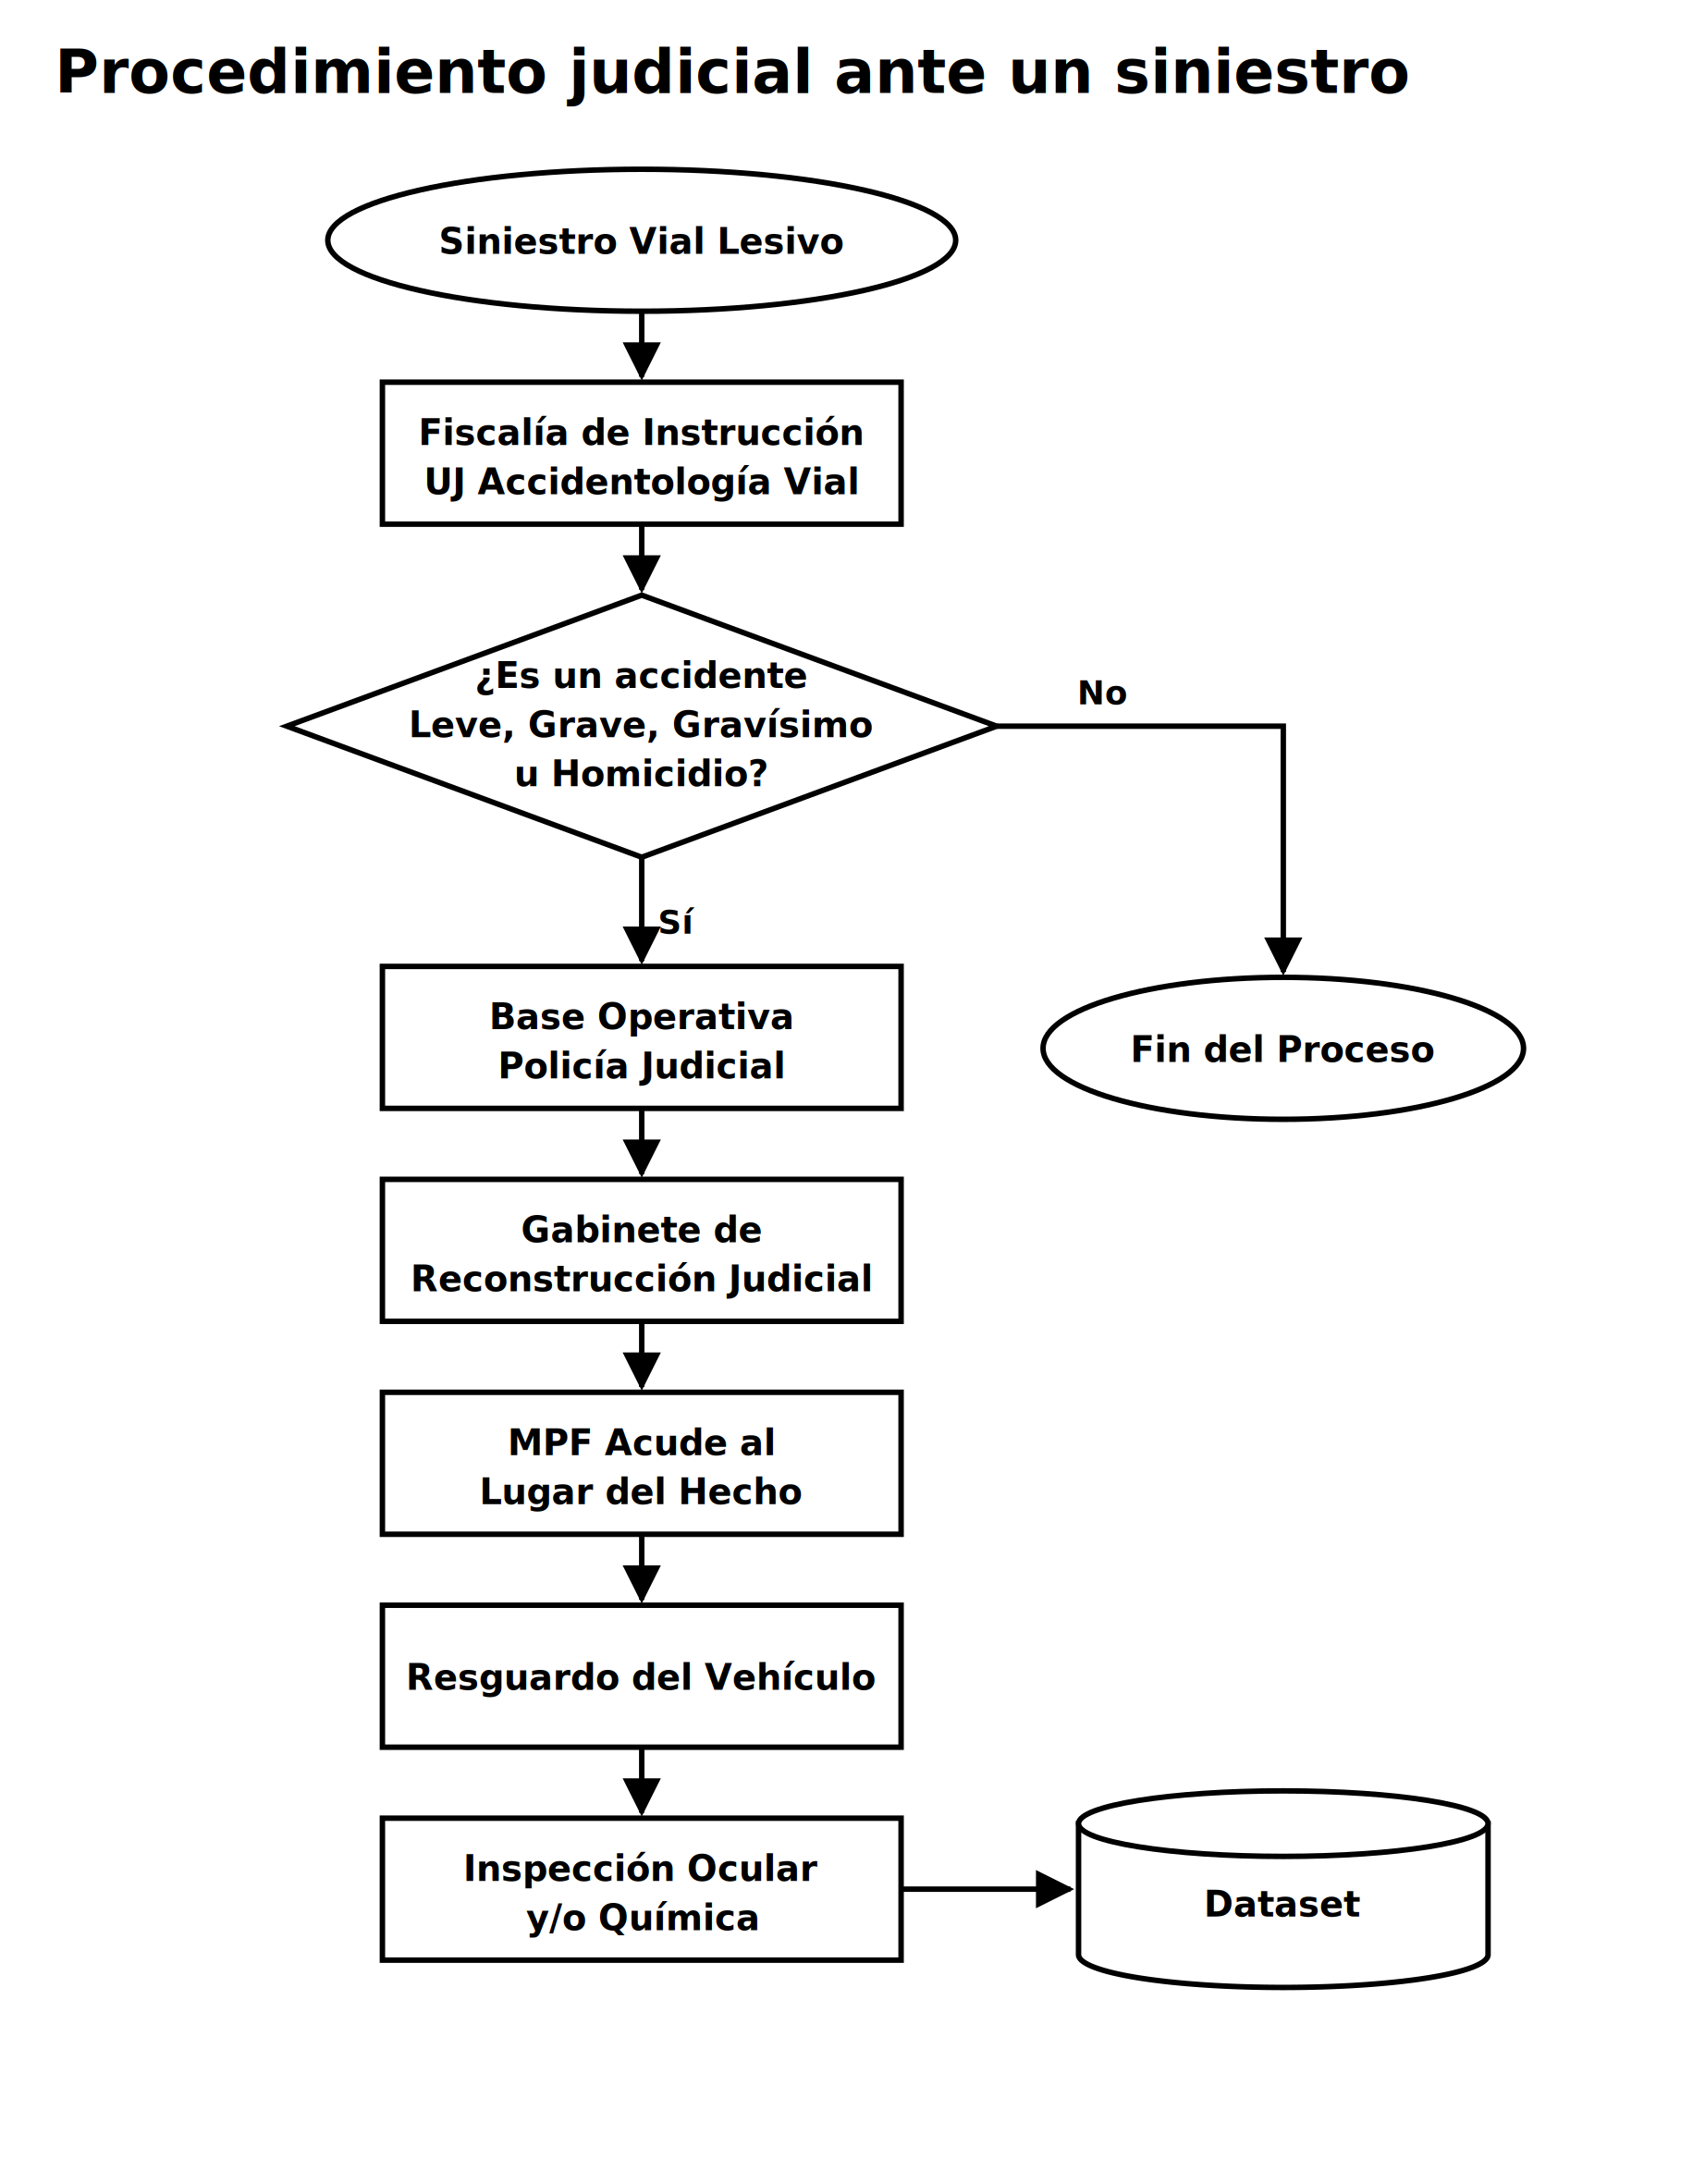
\includegraphics[width=\linewidth]{imagenes/image13.png}
\caption{Procedimiento judicial ante un siniestro vial}
\label{fig:procedimiento-judicial-siniestro}
\end{figure}

El procedimiento judicial tanto en su dimensión administrativa como pericial ante un siniestro vial se inicia con la toma de conocimiento por parte de la fiscalía de instrucción, que opera específicamente a través de las unidades judiciales, en este caso en particular actúa la unidad judicial de accidentología vial (UJ), las cuales practican los primeros actos de la investigación penal preparatoria. Según la calificación legal del hecho, que puede comprender desde lesiones leves hasta homicidio, puede solicitarse la intervención de la base operativa de Policía Judicial para desplegar los recursos técnicos de los gabinetes de reconstrucción criminal y fotografía legal de manera inmediata en el lugar del suceso. Tras realizar los trabajos y los procesos específicos para la preservación de la escena, el vehículo es resguardado en una Unidad Judicial, acto seguido la oficina técnica realiza las inspecciones oculares y químicas correspondientes.

En paralelo, se desarrolla un proceso de gestión documental y carga de información donde personal administrativo, estudiantes de derecho o abogados completan un formulario inicial e integran la declaración del agente policial interviniente. Esta etapa es crítica dentro del proceso dado que es el momento en cual comienzan a adquirirse los datos y la recopilación de estos registros que constituye la formación del conjunto de datos o dataset. En última instancia, esta sistematización digital permite que la información recolectada funcione como el insumo base para el entrenamiento de modelos de inteligencia artificial, en este sentido hay que destacar otro aspecto de vital importancia y es el referido a el tiempo que pasa entre el accidente y la carga de datos en el dataset. Cuando se trabaja con sistemas que realizan \eng{forecasting} la disponibilidad de información en función del tiempo es crítica, en especial en problemas donde necesitamos agregar los datos en bloques discretos de tiempo. Este aspecto se desarrolla con suficiente profundidad más adelante, en cuanto a su influencia en el proceso se contempla esta restricción tanto para la decisión del modelo, la estructura de los dataset, la arquitectura del sistema en su conjunto y los requerimientos y funcionalidades del producto.

\section{Objetivo del proyecto}\label{objetivo-del-proyecto}

Este proyecto integrador consiste en el diseño de un producto \eng{end-to-end}, comenzando desde la transformación de los datos, hasta la implementación de modelos impulsados por inteligencia artificial.

Este producto será concebido desde una mirada transversal y con particular interés en los aspectos que competen al campo de la ingeniería industrial, en ese sentido se puede destacar el uso de metodologías ágiles para la gestión del proyecto de desarrollo, las competencias relacionadas al trabajo con equipos de múltiples disciplinas en especial las que no están vinculadas a las ciencias exactas, el enfoque sistémico para mejorar un proceso donde están implicados no sólo aspectos tecnológicos sino también humanos y normativos. Otro campo de la ingeniería industrial que se tendrá en cuenta para los objetivos de este producto es el relacionado a los sistemas de gestión, en particular para este caso es la Norma ISO/IEC 42001 para el desarrollo responsable, transparente y ético.

De manera general y sin perjuicio de lo antes mencionado, este trabajo incluirá un análisis de los principales aspectos de la gestión de un producto impulsado por inteligencia artificial para \eng{forecasting} de accidentes viales, como gestión de riesgos, análisis y definición de requisitos, escalabilidad del producto, evaluación de impacto y la documentación asociada a sus partes.

%% =====================================================================
%% 6. MARCO TEÓRICO
%% =====================================================================

\chapter{Marco Teórico}\label{marco-teorico}

\section{El Paradigma de Gestión de Producto y la Gestión de Proyecto}\label{el-paradigma-de-gestiuxf3n-de-producto-y-la-gestiuxf3n-de-proyecto}

Para llevar a cabo el diseño y la implementación del sistema de \eng{forecasting} para accidentes viales a nivel de producto mínimo viable (MVP) se debe comenzar observando el problema con una mirada amplia e integral, en el sentido de que este caso tiene una serie de particularidades las cuales restringen o condicionan el desarrollo respecto de un software tradicional. La gestión de un proyecto se mide o se juzga por el cumplimiento de las restricciones internas, es decir que si se termina a tiempo, respetando el alcance y dentro del presupuesto la gestión se considera exitosa o adecuada según el criterio de la triple restricción del PMI \autocite{pmi2021}. Ahora bien, este enfoque no resulta completamente representativo de los desafíos que implica implementar un sistema basado en inteligencia artificial que tiene como principal objetivo ser soporte para la toma de decisiones, esto es debido a que mientras un proyecto tiene un fin predeterminado, desde la perspectiva de la gestión de producto, un producto no se define por el artefacto que lo materializa sino por el valor que entrega a quien lo usa y posee un ciclo de vida dinámico que requiere iteración constante  \autocite{cagan2018} e ir descubriendo y validando el producto a medida que se implementa en entornos reales.

Se tiene entonces un enfoque alternativo y de uso creciente en el mercado que es denominado Gestión de Producto (Product Management) que sugiere que el éxito de un proyecto depende de gestionar adecuadamente el impacto externo y el valor generado (\eng{outcomes}), es decir resolver un problema real del usuario u optimizar un proceso de la organización. Por otra parte se debe analizar la dimensión de la temporalidad, mientras que un proyecto tiene una naturaleza finita establecida por la fecha de inicio y la fecha de finalización, enfocarse en el producto implica asumir que el ciclo de vida es continuo y va evolucionando con las necesidades del usuario a través de mejoras y nuevas funcionalidades.

Otra característica notable que se debe tener en cuenta es el manejo de la incertidumbre y los requerimientos, en un proyecto generalmente se asume la predictibilidad en el sentido de que se intenta definir todo el alcance al principio del mismo, implementar un cambio implica un costo elevado e invertir tiempo en burocracia. Bajo el enfoque en el producto se asume la incertidumbre como constante, especialmente cuando se trabaja con software de inteligencia artificial. No se asume que se conoce lo que necesita o quiere el usuario sino que se lanzan prototipos y se mide la respuesta del usuario adaptando el rumbo con metodologías ágiles. Este último punto condiciona directamente la forma en la que se pueden constituir los equipos de trabajo, enfocarse en el proyecto requiere equipos temporales basados en la disponibilidad de recursos para esa tarea y enfocarse en el proceso permite equipos estables, multidisciplinarios capaces de desenvolverse con profundidad en el dominio del problema.

Este paradigma puede resumirse de la siguiente manera, un \eng{project manager} se enfoca en el cómo y cuándo, coordinando recursos, mitigando riesgos de ejecución, eliminando bloqueos y asegurando el cronograma. Un \eng{product manager} en cambio se enfoca en el qué y el por qué, entendiendo las necesidades del usuario, definiendo la visión a largo plazo, priorizando qué problemas resolver primero y alineando los objetivos del sistema con los del cliente.

El presente trabajo no adopta una postura excluyente entre ambos paradigmas ni los asume como los únicos existentes, sino que propone un enfoque híbrido que garantiza una efectiva adopción tecnológica por parte del usuario final al adaptar perfectamente el producto a sus necesidades y requerimientos al mismo tiempo que los conceptos y las herramientas de la gestión de proyectos permiten seleccionar la tecnología adecuada, identificar riesgos y restricciones, minimizar el uso de recursos y garantizar que no existan desviaciones significativas que condicionen la viabilidad del proyecto.

\section{Niveles de madurez tecnológica (ISO 16290:2013)}\label{niveles-de-madurez-tecnoluxf3gica-iso-162902013}

Originalmente, el concepto de TRL (Technology Readiness Levels) o niveles de madurez tecnológica fue acuñado por la NASA en la década de los 70, sin embargo en 2013 la Organización Internacional de Estandarización (ISO) formalizó este esquema publicando la norma internacional ISO 16290:2013, titulada \enquote{Sistemas espaciales --- Definición de los Niveles de Madurez Tecnológica (TRL) y sus criterios de evaluación}.

La finalidad de esta norma es proporcionar un lenguaje común y riguroso que permita a los investigadores, ingenieros y otras partes interesadas determinar correctamente el estado de desarrollo de una tecnología.

La estructura de la norma se divide en nueve niveles de madurez que comienzan en el nivel 1 con la formulación de los principios básicos y culmina en el nivel 9 con un sistema probado y operando con éxito en un entorno real. Los primeros niveles abordan las etapas conceptuales iniciales de la investigación. En el nivel TRL 1 se identifican los principios científicos básicos que servirán como bases para el desarrollo posterior. En el nivel TRL 2, se formulan las aplicaciones prácticas de dichos principios y se definen los conceptos tecnológicos preliminares. Finalmente el nivel TRL 3 es el último de los niveles de la fase de investigación, donde se lleva a cabo la demostración analítica y experimental de las funciones del sistema mediante una prueba de concepto.

Los niveles desde TRL 4 hasta TRL 7 constituyen la etapa de desarrollo, donde en el TRL 4 se valida el funcionamiento de los componentes del sistema como un conjunto en un entorno de laboratorio para luego en TRL 5 incrementar la fidelidad de las pruebas, validando el funcionamiento en un entorno relevante y controlado. En TRL 6 se exige la demostración de funcionamiento del sistema en un entorno que simule la realidad donde el sistema debe evidenciar un funcionamiento predecible y documentado, para finalmente concluir con la etapa de desarrollo en el nivel TRL 7 donde un prototipo del sistema funcione en un entorno operativo real que garantice que el sistema es capaz de mitigar los riesgos asociados a la aplicación final antes de ser implementado definitivamente.

Finalmente, la escala de madurez de la norma culmina con los niveles orientados a la calificación formal y el uso continuado del sistema. En TRL 8 el sistema ha sido completamente finalizado y calificado para su uso mediante pruebas de aceptación que certifiquen el correcto funcionamiento. Por último, el nivel TRL 9 se alcanza únicamente cuando el sistema real ha sido probado con éxito y se encuentre disponible en el mercado listo para su uso generalizado.

La adopción de esta norma no solo justifica de manera estandarizada el estado actual del desarrollo alcanzado en el proyecto, sino que también traza una hoja de ruta para gestionar la incertidumbre técnica y asegurar la reproducibilidad del proceso de ingeniería implantado.

\section{Gestión de Sistemas de Inteligencia Artificial (ISO 42001:2023)}\label{gestion-de-sistemas-de-inteligencia-artificial-iso-420012023}

La norma internacional ISO 42001:2023, se titula \enquote{Tecnología de la información --- Inteligencia artificial --- Sistema de gestión} y se constituye como el primer estándar internacional dedicado a establecer los requisitos para la creación, implementación, mantenimiento y mejora continua de un sistema de gestión de inteligencia artificial. Su objetivo principal es estructurar un marco de trabajo que permita a las organizaciones desarrollar o utilizar sistemas de Inteligencia Artificial de forma ética, segura y transparente.

Para lograrlo, establece la obligatoriedad de realizar una evaluación de impacto del sistema para documentar y analizar las posibles consecuencias de implementar esta tecnología, así como también establece requisitos rigurosos para la gobernanza de datos, gestión del riesgo y la supervisión humana durante todo el ciclo de vida de la tecnología.

Otro aspecto importante de la norma es el énfasis en la calidad y procedencia de los datos, exigiendo procesos documentados para la preparación, selección y etiquetado de datos utilizados en el entrenamiento de modelos con la finalidad de evitar sesgos algorítmicos.

Además la norma también exige la identificación de las partes interesadas y la definición de políticas organizacionales que minimicen el impacto negativo de los sistemas de IA sobre los individuos y la sociedad.

Su estructura facilita la compatibilidad con otros marcos internacionales de gestión ya establecidos en las organizaciones, como la ISO 9001 para la calidad.

En el contexto de este proyecto, se buscará aplicar la norma como una referencia a las buenas prácticas que facilite un enfoque ético y estructurado, por lo que su intención no es llegar al nivel requerido para una certificación.

Aunque el proyecto no busque una certificación técnica, se adoptarán los controles de la norma para gestionar la calidad y procedencia de los datos suministrados por el Ministerio Público Fiscal desde 2022, contribuyendo a que el entrenamiento de los modelos minimice errores que comprometan la toma de decisiones.

\section{Sistema de Alerta Temprana - SAT}\label{sistema-de-alerta-temprana---sat}

\subsection{Componentes del SAT}\label{componentes-del-sat}

Un sistema de alerta temprana se define como un conjunto de procesos estructurados e integrados que tiene por objetivo proveer al usuario, de manera anticipada, la probabilidad de ocurrencia de un hecho o acontecimiento específico, ésta a veces puede ser una probabilidad pura y otras puede ser un indicador de probabilidad o riesgo relativo bajo diferentes tipos de formatos. En el contexto de este proyecto, el sistema de alerta temprana consiste en una arquitectura de \eng{forecasting} basada en un modelo de inteligencia artificial que procesa datos históricos suministrados por el Ministerio Público Fiscal (MPF) para facilitar la toma de decisiones relacionadas con la asignación de recursos operativos.

Para diseñar un sistema de alerta temprana hay que tener en cuenta cuatro aspectos o componentes fundamentales que juntos explican cómo se relaciona con el problema para el cual fue concebido, estos son: Conocimiento del riesgo, seguimiento y pronóstico, comunicación y capacidad de respuesta.

En cuanto a el conocimiento del riesgo, esto está relacionado al contexto en el cual el sistema operará, es decir a la caracterización de la problemática y la comprensión de las variables que influyen en cómo se asignan recursos cuando suceden siniestros viales, que restricciones existen y qué mejoras podemos esperar luego de implementar el sistema.

Por otra parte tenemos que considerar el seguimiento y pronóstico, aquí se diseñará una arquitectura teniendo en cuenta todos los requisitos y las restricciones que contempla el producto. Se puede optar por modelos de línea de base puros como XGBoost, LightGBM o MLP configurados con hiperparámetros adaptados al procesamiento de series temporales para detección de anomalías y entrenados para hacer regresiones o clasificaciones. También se pueden incluir capas de decisión, que consisten en un post procesamiento determinista de la predicción (esto permite que el usuario ajuste la sensibilidad del SAT) para activar el sistema no solo en función de la salida del modelo sino que tenga en cuenta por ejemplo una capa estadística que usa una comparación Z-Score antes de dar el resultado. Otra alternativa que se contempló para hacer el \eng{forecasting} es el uso de múltiples modelos estructurados bajo una arquitectura de ensamblado ponderado (Weighted Ensemble), que le permitirá al SAT aprovechar las distintas ventajas de cada modelo para identificar patrones de distinta naturaleza y combinarlos en una única predicción. En este sentido es necesario comprender que para un mismo set de datos pueden existir modelos que capturen mejor dependencias de largo plazo, que capturen mejor la estacionalidad, que tengan funciones de probabilidad más suavizadas en la salida y otros que tengan gran explicabilidad como es el caso de los modelos basados en árboles de decisión.

Adicionalmente hay que definir un criterio para transmitir la información al usuario, este es un aspecto crítico de un sistema de alerta temprana porque hay que tener en cuenta en el diseño de experiencia de usuario que el mismo puede interpretar de distinta manera la predicción del modelo, generalmente se tiene la ventaja de que este será un experto en el dominio y tendrá una referencia basada en años de experiencia para comparar con la predicción, al mismo tiempo se tiene la desventaja de que es un usuario que no tiene conocimientos avanzados de estadística o de Machine Learning lo que hace casi obligatorio que el producto se implemente en un formato fácil de consumir como por ejemplo la codificación RAG (Red, Amber, Green).

El último componente que hay que tener en cuenta para diseñar un sistema de alerta temprana es la capacidad de respuesta, esto significa que cada tipo de alerta debe estar ligado a un plan de acción en concreto que debe llevar a cabo el personal del Ministerio Público Fiscal. Este punto excede el alcance de este trabajo en particular dada la complejidad y especificidad de los procesos que lleva a cabo tal institución. Queda pendiente para trabajos que pudieran realizarse en el futuro evaluar el impacto del sistema de \eng{forecasting} en el uso de recursos.

\subsection{Umbrales de Alerta}\label{umbrales-de-alerta}

La operativización de un SAT requiere la segmentación de las señales de riesgo mediante umbrales (\eng{thresholds}) basados en métricas estadísticas de control según el tipo de problema al que se está enfrentado y en ocasiones a las preferencias de los usuarios finales.

La metodología más validada tanto en el ámbito académico como en el mercado para escenarios similares consiste en segmentar según tres o cuatro niveles de riesgo con colores predefinidos como sigue:

\begin{description}
  \item[Nivel verde (línea de base).] Corresponde al estado estacionario del sistema. Los modelos predictivos proyectan que las variables se mantendrán dentro de los intervalos de confianza históricos y los límites de control aceptables.
  \item[Nivel amarillo (prevención).] Se activa ante la detección de desviaciones estadísticas sutiles o tendencias que indican una deriva del comportamiento normal. Este nivel no implica un riesgo inminente, sino la necesidad de que el tomador de decisiones se mantenga un poco más alerta.
  \item[Nivel naranja (alerta).] Se establece cuando los algoritmos determinan una alta probabilidad matemática de que las variables más significativas vulneren los umbrales de seguridad en un horizonte temporal cercano. Este nivel activa los procesos que el usuario haya predefinido o considere adecuados para esta alerta según su experiencia.
  \item[Nivel rojo (crítico).] Representa la inminencia o la ocurrencia efectiva del evento adverso. En este nivel, el sistema pone en conocimiento del usuario que está ante una anomalía significativa y que debe prepararse o tomar decisiones en proporción.
\end{description}

\subsection{Características de un SAT eficiente}\label{caracteruxedsticas-de-un-sat-eficiente}

La utilidad operativa de un SAT está condicionada por su horizonte de predicción. Los sistemas se dividen en dos categorías principales, las alertas inmediatas en tiempo real y las alertas predictivas por bloques o franjas de tiempo.

Las alertas inmediatas operan bajo un paradigma reactivo en tiempo real (\eng{near real-time}). Se configuran mediante algoritmos de detección de anomalías puntuales y se activan en el instante exacto en que un parámetro supera un límite preestablecido. Ofrecen una certidumbre matemática elevada respecto a la existencia del evento, pero reducen el margen de maniobra a cero dado que no le da tiempo suficiente al usuario para anticiparse y actuar.

Por otra parte, las alertas predictivas por bloques o franjas de tiempo discretas utilizan modelos supervisados o arquitecturas de aprendizaje profundo para proyectar la serie temporal hacia un horizonte futuro (próximos bloques de tiempo). Esta ventana temporal proporciona un diferencial de gran utilidad para la gestión de riesgos, permitiendo al usuario tomar decisiones anticipándose por medio de una estrategia de mitigación planificada.

El diseño a nivel algorítmico de un SAT basado en inteligencia artificial enfrenta una restricción metodológica conocida como el dilema entre la tasa de verdaderos positivos (\emph{recall}) y la tasa de valor predictivo positivo (precisión) \autocite{fawcett2006}.
% TODO(bib): en el original también se citaba "Saito y Rehmsmeier (2015)", que no figuraba en la lista de Bibliografía del documento original; agregarla a bibliografia.bib con sus datos completos.
Un sistema configurado y entrenado con una sensibilidad (\eng{recall}) extrema minimizará la ocurrencia de falsos negativos, asegurando la captura de cualquier anomalía, no obstante, incrementará exponencialmente los falsos positivos, induciendo el fenómeno operativo denominado fatiga de alertas, el cual degrada la confianza del usuario \autocite{ancker2017} dado que siempre está expuesto a una alerta. Por el contrario, la maximización de la precisión reduce las falsas alarmas, pero eleva el riesgo de perderse eventos críticos (falsos negativos) sin emitir alerta alguna. La calibración de los umbrales de decisión debe responder, por tanto, a una comprensión profunda de que implica alertar de cierta manera al tomador de decisiones, y cómo las mismas impactan en el servicio que estos prestan a los ciudadanos.

\section{Forecasting}\label{forecasting}

\subsection{Deep Learning y Machine Learning}\label{deep-learning-y-machine-learning}

En el campo del \eng{forecasting} para pronóstico basado en series temporales se pueden distinguir de manera predominante dos tecnologías para el tratamiento, procesamiento, y generación de modelos predictivos, por un lado tenemos al Aprendizaje Automático clásico o Machine Learning y por otro a Aprendizaje Profundo o Deep Learning. Además de la obvia distinción terminológica tenemos diferencias fundamentales en cómo estas técnicas procesan la información, usan diferentes arquitecturas a nivel algoritmos y tienen diferentes requisitos de infraestructura tecnológica que en ocasiones es determinante a la hora de elegir entre una o la otra.

El Machine Learning es una serie o conjunto de algoritmos y modelos que permiten a los sistemas identificar patrones como secuencias, anomalías, ciclos, grupos, tendencias y realizar inferencias a partir de datos sin que estos algoritmos sean programados explícitamente para cada tarea. En el contexto de este proyecto estas técnicas permiten implementar enfoques particularmente robustos dadas las características particulares que este dominio requiere y en especial puede aportar ventajas muy valoradas que se mencionan oportunamente.

Desde el punto de vista teórico, el Machine Learning se apalanca principalmente de la ingeniería de variables (\eng{feature engineering}), donde el conocimiento del dominio en este caso el referido a accidentología vial y su correspondiente proceso judicial permite extraer, construir y modelar características específicas para alimentar modelos como árboles de decisión, LightGBM o XGBoost. Este tipo de implementaciones tiene una ventaja muy relevante respecto de otras técnicas y tecnologías, y es que el Machine Learning tiene capacidad de Explicabilidad (XAI) al no operar como una caja negra absoluta, es decir que permitiría a los analistas judiciales, auditores, y usuarios en general comprender la lógica que subyace a una predicción, garantizando así que el producto esté alineado con los criterios de transparencia exigidos por la norma ISO/IEC 42001 (Cláusulas A.7.3 / A.7.4 / A.7.5).

El Deep Learning en cambio constituye una subdisciplina del Machine Learning inspirada en la estructura neurobiológica de una neurona del cerebro humano, utiliza redes neuronales artificiales constituidas por una capa de entrada, múltiples capas ocultas conectadas en simultáneo entre sí y estas últimas a una capa de salida que le permite aprender representaciones complejas de datos. A diferencia del Machine Learning clásico el Deep Learning tiene la capacidad intrínseca de realizar la extracción de características de forma automática, identificando relaciones no lineales y todo tipo de dependencias temporales profundas. Dentro del espectro del Deep Learning para series temporales se pueden destacar algunas arquitecturas como las redes de Perceptrón Multicapa (MLP) y las redes recurrentes LSTM (Long Short Term Memory) cada una de las cuales tiene requisitos y limitaciones específicas que se deben tener en cuenta antes de implementarlas.

\subsection{Árboles de decisión}\label{uxe1rboles-de-decisiuxf3n}

Un árbol de decisión es un modelo predictivo o una familia de modelos que segmenta el espacio de los datos de manera recursiva basándose en decisiones binarias, esto genera una estructura jerárquica de ramas y hojas que permite una representación intuitiva del proceso de decisión que favorece la explicabilidad del modelo. Estos árboles individuales suelen presentar limitaciones de varianza y riesgo de sobreajuste, estos inconvenientes pueden ser resueltos mediante el uso de diferentes técnicas como el ensamble mediante Boosting.

El método del Boosting consiste en plantear que un algoritmo de aprendizaje débil, es decir que puede predecir levemente mejor que realizar una predicción aleatoria, puede convertirse en un modelo con un gran rendimiento a través del uso de este método. Básicamente consiste en un método de aprendizaje por ensamble que combina una serie de aprendizajes poco asertivos para generar un modelo con una precisión elevada. Este entrenamiento es realizado de forma secuencial de manera que cada modelo corrige los errores cometidos por su predecesor, por ende la idea principal es combinar varios modelos individuales y unificarlos para mejorar la precisión general.

Otra una técnica de amplio uso en el campo del Machine Learning llamada Bagging que se explica a continuación. Tal metodología implica tomar los aprendizajes débiles para entrenar el modelo general en paralelo, de tal forma que se entrenan varios árboles de forma independiente y en simultáneo con distintos conjuntos de datos. El resultado final se obtiene mediante un promedio de las predicciones o una votación dependiendo de si el problema es de clasificación o regresión.

Si se quiere comparar estas dos metodologías se debe tener en cuenta que en el Boosting el entrenamiento es secuencial y cada modelo trata de corregir los errores del modelo anterior, aumentando así la precisión global del estudio. Sin embargo, es más propenso al sobreajuste, por lo que es necesario tomar precauciones a la hora de incorporar nuevos árboles. Esta es una desventaja respecto al Bagging y por eso, esta opción puede ser mejor para conjuntos de datos muy complejos con muchas observaciones atípicas.

\begin{figure}[htbp]
\centering
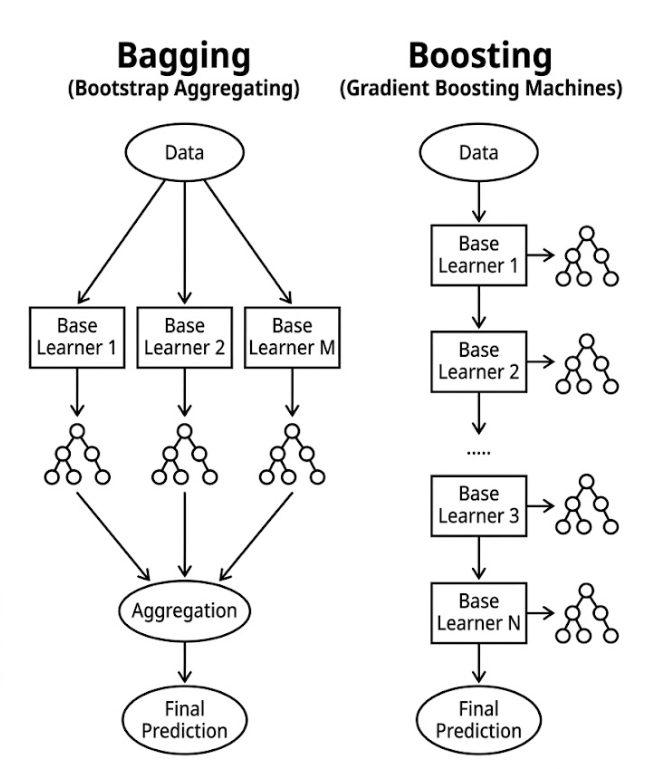
\includegraphics[width=0.59\linewidth]{imagenes/image10.png}
\caption{Arquitectura de bagging comparada con la de gradient boosting}
\label{fig:arquitectura-de-bootstrap-comparada-con-}
\notaflot{\fuentepropia{} en base a la arquitectura de Bagging y Boosting.}
\end{figure}

\subsection{LightGBM y XGBoost}\label{lightgbm-y-xgboost}

En el contexto de técnicas de aprendizaje supervisado las metodologías basadas en Gradient Boosting (Figura 2.1) mencionadas anteriormente han ido evolucionando para optimizar su funcionamiento en lo referido a limitaciones computacionales en casos donde se necesita trabajar con volúmenes masivos de datos o problemas que tienen de base una alta dimensionalidad, por ejemplo proyectos en donde el modelo tienen que entrenar a partir de 65 características (columnas en el dataset) como lo es el caso de los datos originales de este proyecto de siniestros viales. Para resolver estas deficiencias surgieron arquitecturas optimizadas, las dos más notables son XGBoost (Extreme Gradient Boosting) y LightGBM (Light Gradient Boosted Machine) que destacan por incorporar innovaciones vitales en la función objetivo, la gestión del hardware y las estrategias de división de nodos.

Sobre XGBoost se menciona que fue desarrollado por Tianqi Chen y Carlos Guestrin en 2016, y es una implementación de alto desempeño de Gradient Boosting. Sus fortalezas se basan en dos pilares principales, la regularización matemática de la función objetivo y la optimización del sistema a nivel de hardware. A diferencia de otros modelos como XGBoost añade un término de regularización formal $\Omega$ a la función objetivo para controlar la complejidad y extensión de los árboles, esto evita el sobreajuste (\eng{overfitting}). La función objetivo se define según la \cref{eq:xgb-objetivo}:

\begin{equation}
\mathcal{L}^{(t)} = \sum_{i=1}^{n} l\left(y_i,\, \hat{y}_i^{(t-1)} + f_t(x_i)\right) + \Omega(f_t)
\label{eq:xgb-objetivo}
\end{equation}

\noindent donde $\mathcal{L}^{(t)}$ es la función objetivo evaluada en la iteración $t$, y:

\begin{itemize}
    \item $n$: cantidad de observaciones del conjunto de entrenamiento.
    \item $y_i$: valor observado (real) de la variable objetivo para la observación $i$.
    \item $\hat{y}_i^{(t-1)}$: predicción acumulada del modelo para la observación $i$ luego de $t-1$ iteraciones.
    \item $x_i$: vector de características (predictores) de la observación $i$.
    \item $f_t$: nuevo árbol incorporado en la iteración $t$, de modo que $f_t(x_i)$ es la corrección que dicho árbol aporta sobre la predicción previa.
    \item $l(\cdot)$: función de pérdida diferenciable y convexa que cuantifica el error entre el valor observado $y_i$ y el predicho.
    \item $\Omega(f_t)$: término de regularización que penaliza la complejidad del árbol $f_t$, definido como $\Omega(f) = \gamma T + \tfrac{1}{2}\lambda \lVert w \rVert^{2}$, siendo $T$ el número de hojas, $w$ el vector de pesos asignados a esas hojas, y $\gamma$ y $\lambda$ los hiperparámetros que controlan la magnitud de la penalización.
\end{itemize}

Para optimizar esta función rápidamente con cualquier función de pérdida de segundo orden, XGBoost aplica una expansión en serie de Taylor de segundo grado. Esto permite que el algoritmo utilice tanto el gradiente de primer orden ($g_i$) como el gradiente de segundo orden (Hessiano, $h_i$), acelerando drásticamente la convergencia matemática.

\begin{equation}
\mathcal{L}^{(t)} \simeq \sum_{i=1}^{n} \left[ l\left(y_i,\, \hat{y}_i^{(t-1)}\right) + g_i f_t(x_i) + \tfrac{1}{2} h_i f_t^{2}(x_i) \right] + \Omega(f_t)
\label{eq:xgb-taylor}
\end{equation}

\noindent donde, además de los términos ya definidos:

\begin{itemize}
    \item $l\left(y_i, \hat{y}_i^{(t-1)}\right)$: pérdida de la predicción acumulada hasta la iteración anterior. Al no depender de $f_t$, constituye un término constante que puede omitirse durante la optimización.
    \item $g_i = \partial_{\hat{y}^{(t-1)}}\, l\left(y_i, \hat{y}_i^{(t-1)}\right)$: gradiente de primer orden de la función de pérdida respecto de la predicción acumulada; indica la dirección y magnitud del error que el nuevo árbol debe corregir.
    \item $h_i = \partial^{2}_{\hat{y}^{(t-1)}}\, l\left(y_i, \hat{y}_i^{(t-1)}\right)$: gradiente de segundo orden o hessiano; mide la curvatura de la pérdida y pondera cuán agresiva debe ser esa corrección.
\end{itemize}

En cuanto a las características de este sistema hay algunos aspectos destacables a tener en cuenta, el primero de ellos es el soporte para valores faltantes (Sparsity-aware Split Finding) en el cual XGBoost asigna automáticamente una dirección por defecto en cada nodo para los datos ausentes basándose en cuál dirección minimiza la pérdida durante el entrenamiento. Otra es la estructura de bloques en paralelo, en esta los datos se almacenan en memoria en formato de bloques ordenados por columnas, esto permite calcular las divisiones de diferentes variables de forma paralela en la CPU. Por último se tiene acceso consciente en caché (Cache-aware Access) que le permite a XGBoost minimizar los fallos de caché asignando hilos de ejecución de manera que los gradientes se puedan leer en bloques continuos.

Por otra parte se tiene a LightGBM (Light Gradient Boosted Machine), el cual fue diseñado por Microsoft en 2017 y concebido específicamente para superar a XGBoost en velocidad de entrenamiento y consumo cuando se trabaja en proyectos de una gran dimensionalidad. De manera general que sus ventajas se basan en muestreo matemático y en una variante en la forma en la que crecen los árboles respecto del modelo antes mencionado.

Un aspecto fundamental que hay que distinguir cuando se implementan árboles en modelos predictivos es el referido al crecimiento por hojas (Leaf-wise) en contraposición al crecimiento por niveles (Level-wise). La mayoría de los algoritmos de boosting incluyendo las primeras versiones de XGBoost expanden los árboles a medida que van entrenando por el método de crecimiento por nivel, esto significa que todas las hojas de un nivel se generan simultáneamente manteniendo el árbol balanceado pero incurriendo en el riesgo de calcular divisiones ineficientes en ramas que tienen poco gradiente. LightGBM en cambio utiliza una estrategia distinta, el algoritmo busca y divide únicamente la hoja que genera mayor reducción de pérdida global, sin importar la profundidad. Este método genera árboles asimétricos y profundos que reducen rápidamente el error residual, siendo matemáticamente más eficientes a costa de tener una mayor tendencia a sobreajuste en muestras más chicas. LightGBM mitiga este efecto proporcionando un hiperparámetro que pone un límite estricto a la profundidad máxima del árbol.

\begin{table}[htbp]
\centering
\caption{Comparación entre XGBoost y LightGBM}
\label{tab:comparacion-xtreme-gradient-boosting-vs-}
\small
\begin{tabularx}{\textwidth}{@{}p{3.1cm}XX@{}}
\toprule
\textbf{Dimensión técnica} & \textbf{XGBoost} & \textbf{LightGBM} \\
\midrule
Estrategia de crecimiento & Normalmente \eng{level-wise} (por niveles) & \eng{Leaf-wise} (por hojas con mayor ganancia) \\
División de variables continuas & Percentiles ordenados (\eng{Weighted Quantile Sketch}) & Basado en histogramas optimizados (\eng{bins} fijos) \\
Manejo de \eng{sparse} & Algoritmo guiado por dispersión (\eng{sparsity-aware}) & Reducción por exclusión de características (EFB) \\
Técnica de muestreo & Muestreo aleatorio tradicional (\eng{subsampling}) & Muestreo unilateral por gradientes (GOSS) \\
Consumo de memoria RAM & Moderado-alto (guarda valores exactos o cuantiles complejos) & Extremadamente bajo (enteros de 8 bits para los \eng{bins}) \\
Velocidad de cómputo & Alta (optimización por bloques y caché) & Muy alta (GOSS, EFB e histogramas) \\
\bottomrule
\end{tabularx}
\notaflot{\fuentepropia{}, según comparación de XGBoost contra LightGBM.}
\end{table}

\subsection{Ventanas Deslizantes (Sliding Windows)}\label{ventanas-deslizantes-sliding-windows}

Comúnmente en los casos de aprendizaje automático más tradicionales, los modelos asumen que un determinado conjunto de datos tiene todos sus registros independientes y distribuidos uniformemente, esto significa por ejemplo que el orden en el cual se tienen los registros es irrelevante, que se tienen igual cantidad de etiquetas de cada clase cuando se quiere clasificar, entre otras implicaciones. Ahora bien, cuando se requiere hacer \eng{forecasting} o aplicar algún tipo de modelo predictivo para series temporales, los datos representan una dependencia cronológica que hace al fondo del problema, es decir, que de alguna manera el estado de una variable en el instante actual está condicionado o relacionado con sus estados cuantitativos en instantes previos. Para poder hacer uso de modelos como XGBoost, LightGBM o algún otro que se considere conveniente es obligatorio reestructurar el dataset de registros clásicos en formato tabla de hechos (Fact Table) a un formato matricial que capture esa estructura secuencial. El método que permite lograr este resultado es comúnmente conocido como enfoque de Ventanas Deslizantes, Lagging, o Ventanas de Retardo. Para el caso en específico de su uso en Machine Learning también se conoce como transformación de datos por formulación autorregresiva supervisada.

Dado que el tipo de problema que implica crear un sistema de \eng{forecasting} impulsado por inteligencia artificial para siniestros viales es de naturaleza multivariada se requerirá implementar el concepto de ventanas deslizantes para todas las características del dataset original. Específicamente se quiere decir que el número de víctimas o el riesgo de que existan accidentes en un tiempo determinado está relacionado con múltiples variables como lo pueden ser el clima, historial de siniestros previos, lugar, día y hora, festividades, etc, y que por lo tanto un registro deberá contener información tanto del presente como del pasado.

La aplicación del método de ventanas deslizantes en un entorno multivariado requiere una generalización geométrica y matemática del proceso de rezago (lagging), transformando tensores temporales en matrices tabulares aptas para algoritmos de aprendizaje automático. A continuación se formula el método mencionado ut supra.

Supóngase que se dispone de un sistema con $K$ variables distintas medidas simultáneamente a lo largo de $T$ instantes de tiempo. En cada paso de tiempo $t$ las observaciones no son un número escalar, sino un vector de observaciones $\mathbf{z}_t \in \mathbb{R}^{K}$:

\begin{equation}
\mathbf{z}_t = \left[ z_{t,1},\; z_{t,2},\; \dots,\; z_{t,K} \right]^{\top}
\label{eq:vector-observaciones}
\end{equation}

El conjunto de datos completo se representa como una secuencia cronológica de vectores o, equivalentemente, como una matriz de datos original $\mathbf{Z}$ de dimensiones $T \times K$:

\begin{equation}
\mathbf{Z} =
\begin{bmatrix}
\mathbf{z}_1^{\top} \\
\mathbf{z}_2^{\top} \\
\vdots \\
\mathbf{z}_T^{\top}
\end{bmatrix}
=
\begin{bmatrix}
z_{1,1} & z_{1,2} & \dots  & z_{1,K} \\
z_{2,1} & z_{2,2} & \dots  & z_{2,K} \\
\vdots  & \vdots  & \ddots & \vdots  \\
z_{T,1} & z_{T,2} & \dots  & z_{T,K}
\end{bmatrix}
\label{eq:matriz-datos}
\end{equation}

Este mecanismo convierte un flujo continuo multidimensional en una matriz plana estándar donde cada columna de la nueva matriz pasa a representar una entidad acoplada temporalmente. Puesto que esta transformación es de vital importancia para este proyecto se adjunta a continuación y a mera forma ilustrativa una tabla que representa figurativamente el tratamiento que se le dio a los datos de accidentes viales.

\begin{longtable}[]{@{}lccccccc@{}}
\caption{Ilustración del método de retardos con ventana deslizante}
\label{tab:ilustracion-sobre-el-metodo-de-retardos-}\\
\toprule\noalign{}
\textbf{Fecha} & \textbf{Día} & \textbf{Temp} & \textbf{Lesiones} & \textbf{Inercia} & \textbf{Lagg\_1} & \textbf{Lagg\_3} & \textbf{Víctimas} \\
\midrule\noalign{}
\endfirsthead
\toprule\noalign{}
\textbf{Fecha} & \textbf{Día} & \textbf{Temp} & \textbf{Lesiones} & \textbf{Inercia} & \textbf{Lagg\_1} & \textbf{Lagg\_3} & \textbf{Víctimas} \\
\midrule\noalign{}
\endhead
\bottomrule\noalign{}
\endlastfoot
01/06 & L & 24 & 0 & 0 & 0 & 0 & 0 \\
02/06 & M & 24,5 & 0 & 0 & 0 & 0 & 0 \\
03/06 & X & 22 & 2 & 0 & 0 & 0 & 1 \\
04/06 & J & 23 & 0 & 1 & 1 & 1 & 0 \\
05/06 & V & 21,7 & 3 & 0 & 0 & 1 & 3 \\
06/06 & S & 20 & 2 & 2,2 & 3 & 4 & 1 \\
07/06 & D & 14,8 & 3 & 2,7 & 1 & 4 & 4 \\
08/06 & L & 12 & 0 & 3,1 & 4 & 8 & 0 \\
09/06 & M & 16,5 & 0 & 0 & 0 & 5 & 0 \\
10/06 & X & 22 & 0 & 0 & 0 & 4 & 0 \\
11/06 & J & 22,2 & 0 & 0 & 0 & 0 & 0 \\
12/06 & V & 21,9 & 3 & 0 & 0 & 0 & 1 \\
\end{longtable}

\notaflot{\fuentepropia{}.}

En la \cref{tab:ilustracion-sobre-el-metodo-de-retardos-} se puede observar cómo queda formateado un set de datos bajo la estructura de formulación autorregresiva supervisada, nótese que cada fila contiene información del presente como el día y la temperatura, e información del pasado como los retardos (laggs) y la inercia. Luego se registra la cantidad de víctimas bajo esas condiciones, el modelo que se use intentará predecir las víctimas conociendo el contexto disponible.

\subsection{AutoGluon y Transformers}\label{auto-gluon-y-transformers}

Existe un punto de tangencia entre la arquitectura Transformer (modelos con pesos pre entrenados a partir del cual se realiza un nuevo entrenamiento específico para el caso) y el ecosistema conocido como AutoGluon-TimeSeries (Auto Machine Learning) y es que la combinación de estas dos tecnologías genera un cambio de paradigma fundamental a la hora de realizar pronósticos de series temporales, superando la instancia de modelos estadísticos tradicionales y consolidando como estado del arte a modelos fundacionales de aprendizaje profundo global.

Los Transformers, son caracterizados por su mecanismo de auto atención escalada que les otorga una capacidad propia o intrínseca para capturar dependencias no lineales de largo plazo, y dinámicas cronológicas relativamente complejas sin verse comprometidos a nivel uso de memoria, o por el desvanecimiento del gradiente como es el caso de las primeras arquitecturas recurrentes.

Por otra parte, AutoGluon para series temporales se beneficia de integrar de manera nativa arquitecturas basadas en atención, como la familia de modelos Chronos (Chronos 2, Chronos Bolt, etc) las cuales reestructuran el análisis numérico continuo propio de una serie temporal como una tarea de modelado de lenguaje autorregresivo, similar a los utilizados por los LLM (Large Language Model) actuales mediante procesos de escalamiento local y cuantización uniforme sobre un vocabulario de tokens.

La estrategia propuesta para el uso de AutoGluon no implica que un modelo único domine todos los escenarios reales posibles, es de suponer que según la naturaleza del problema que se enfrente, las limitaciones de información que se disponga, y el nivel de certidumbre requerida condicione la selección del modelo. Es por eso que el objetivo principal de esta tecnología es proveer al usuario una multiplicidad de modelos subdivididos en tres categorías estructurales que se definen a continuación.

Modelos Globales de Aprendizaje Profundo (Global Deep Learning): Modelos que comparten un único set de parámetros para todas las series temporales del dataset. Aquí se ubican los Transformers de secuencia como Chronos y PatchTST, y las redes neuronales recurrentes clásicas como DeepAR de GluonTS.

Modelos Locales Estadísticos (Local Statistical Models): Modelos univariados tradicionales que se ajustan de manera aislada e independiente para cada serie individual, como ARIMA, ETS y Theta de la librería Stats Forecast.

Modelos Tabulares Autoregresivos (Tree-Based Regressors): Mediante estrategias recursivas o por pasos, AutoGluon transforma las series a formato tabular mediante ventanas deslizantes según como se explicó en párrafos anteriores e inyecta estos datos en las arquitecturas optimizadas de LightGBM, XGBoost y CatBoost a través de AutoGluon-Tabular.

\subsection{Ensamble Ponderado (Weighted Ensemble)}\label{ensamble-ponderado-weighted-ensemble}

La fase final del algoritmo no consiste en seleccionar un único modelo individual con el mejor desempeño, sino en construir el denominado Ensamble Ponderado (Weighted Ensemble) que realiza la predicción final.

\begin{equation}
\hat{y}_{\text{ensemble}} = \sum_{m=1}^{M} w_m \cdot \hat{y}_m,
\qquad \text{sujeto a } \sum_{m=1}^{M} w_m = 1 \text{ y } w_m \geq 0
\label{eq:ensamble-ponderado}
\end{equation}

\noindent donde:

\begin{itemize}
    \item $\hat{y}_{\text{ensemble}}$: predicción final del ensamble, obtenida como combinación lineal de las predicciones de los modelos base.
    \item $M$: cantidad total de modelos base que integran el ensamble.
    \item $m$: índice que identifica a cada modelo base, con $m = 1, \dots, M$.
    \item $\hat{y}_m$: predicción generada individualmente por el modelo base $m$.
    \item $w_m$: peso asignado al modelo $m$, que representa su contribución relativa a la predicción final. AutoGluon determina estos pesos según el desempeño de cada modelo sobre el conjunto de validación, de manera que los modelos más precisos reciben mayor ponderación.
\end{itemize}

\noindent Las restricciones $\sum_{m=1}^{M} w_m = 1$ y $w_m \geq 0$ garantizan que la combinación sea convexa: los pesos no pueden ser negativos y su suma debe ser unitaria, de modo que la predicción del ensamble permanece dentro del rango de las predicciones individuales y se preserva la escala de la variable objetivo. Un peso $w_m = 0$ implica que el modelo $m$ queda efectivamente excluido del ensamble.

Esta última ecuación muestra que la predicción final es el resultado de agregar las predicciones de cada uno de los diferentes modelos según el peso ponderado que le asigna el método de AutoGluon.

De este modo el uso y la implementación de este modelo especializados para \eng{forecasting} en series temporales no solo es un software aislado sino que permite operativizar mediante un framework de trabajo la automatización del procesamiento de datos, la alineación temporal, el uso de transformers permitiendo el ajuste fino (modificaciones específicas al modelo original del transformer) y el ensamble ponderado final.

\begin{figure}[htbp]
\centering
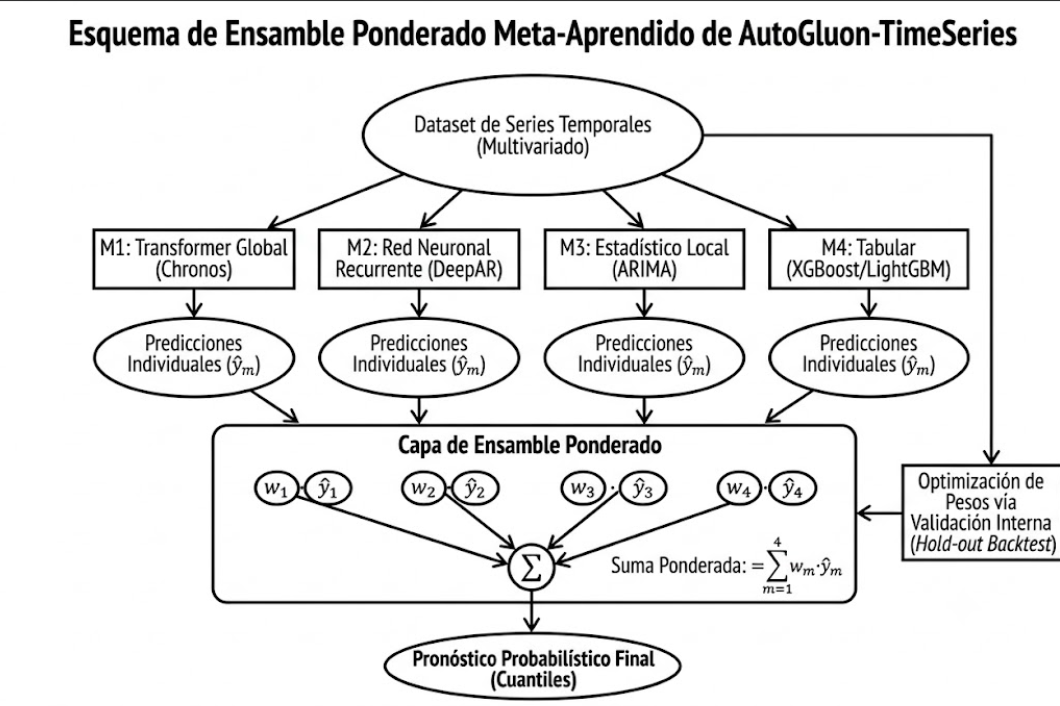
\includegraphics[width=\linewidth]{imagenes/image21.png}
\caption{Esquema del ensamble ponderado de AutoGluon}
\label{fig:esquema-de-ensamble-ponderado-de-autoglu}
\notaflot{\fuentepropia{} según la documentación del repositorio de AutoGluon-TimeSeries.}
\end{figure}

%% =====================================================================
%% 7. DESARROLLO DEL PRODUCTO
%% =====================================================================

\chapter{Desarrollo del Producto}\label{desarrollo-del-producto}

\section{El Problema}\label{el-problema}

Como se mencionó en las etapas introductorias de este proyecto el punto central del problema que se intenta resolver es la gran demanda a la que se enfrenta todos los días el personal del MPF en términos de toma de decisiones para la gestión de tareas y recursos. Los accidentes viales son eventos que tienen escasa probabilidad de suceder en comparación con otros eventos que también gestiona el Ministerio Público Fiscal, sin embargo tienen una característica que los distingue en gran medida de estos últimos, y es que genera un gran impacto a nivel demanda de recursos. Cuando hablamos de ellos, es importante destacar que tal demanda no es uniforme, es decir, dado que cada accidente tiene particularidades propias de la naturaleza del mismo dos de ellos pueden implicar tanto distinta cantidad como distinto recurso propiamente dicho. A esto debe agregarse también el hecho de que la ventana de tiempo para asignar no solo es muy limitada en el tiempo si no que puede ser determinante en cuanto al proceso penal. Entrando específicamente en qué recursos se deben gestionar se puede destacar tanto el personal principal propio del MPF como lo pueden ser, oficiales de justicia, peritos especializados, la policía, como terceros pero fuertemente vinculados como el personal de tránsito, funcionarios municipales, y personal de clínicas y hospitales.

Se tiene así entonces un problema de gran complejidad, que surge de la combinación de tres aspectos y características fundamentales. El proceso es altamente demandante a nivel coordinación de personal y recursos técnicos, también es requisito sine qua non hacerlo con la máxima velocidad y precisión porque está vinculado al posible proceso penal y por último es un evento que hasta ahora era impredecible por lo que el MPF está obligado a sobre dimensionar sus operaciones referidas a accidentes viales. Queda de esta manera definido el principal punto de dolor del usuario siendo esto la motivación de orden uno para ese proyecto.

Teniendo en cuenta lo anteriormente expuesto sería posible intuir que una forma de solucionarlo pueda ser el uso de tecnología, pero esto es parcialmente cierto. Desde el punto de vista de la ingeniería industrial este problema debe considerar el enfoque de personas, procesos y tecnología (PPT) el cual sugiere que estos son los tres aspectos clave que hay que gestionar para solucionar el problema de la forma apropiada.

Si se analiza la dimensión de las personas se debe destacar que el dominio de los usuarios tiene limitaciones determinantes en cuanto a conocimiento específico de herramientas de software o modelos estadísticos avanzados, esto sin duda impacta en cómo se diseñará el producto en términos de explicabilidad y experiencia de usuario. En lo referido a los procesos se destaca especialmente la disponibilidad de información en bloques agregados y el poco volumen de datos existentes. Finalmente en la dimensión tecnológica se debe tener en cuenta aspectos de seguridad informática, normativas, limitarse al uso de tecnología de código abierto, escalabilidad, y mantenimiento de la misma a largo plazo. La conjunción de estos tres aspectos generará una serie de opciones y alternativas para seleccionar las mejores tecnologías que se adapten a los procesos que protagonizan las personas.

Anteriormente se mencionó que el problema estaba definido por tres características fundamentales, es altamente demandante en recursos, requiere velocidad y precisión, y no es posible saber cuándo se va a requerir todo el proceso para accidentes viales. Es en este último punto donde se decidió diseñar un sistema de alerta temprana basado en \eng{forecasting} e impulsado por inteligencia artificial, con la hipótesis de que prever con cierto grado de anticipación cuando hay más riesgo de ocurrencia de accidentes viales será de gran utilidad para planificar el futuro y mejorar notablemente las operaciones del MPF.

\section{Los datos}\label{los-datos}

La correcta carga de datos es un aspecto clave para el funcionamiento del sistema, si lo pensamos detenidamente, introducir información errónea o una mala planificación de los datos que vamos a tomar pueden comprometer la integridad de todo el proyecto, anulando el valor de los análisis, realizando malas predicciones debido a información errónea y condicionando a futuro todo el ciclo de vida del producto.

Entonces, los datos son recopilados por el personal del Ministerio Público Fiscal y cargados a la base de datos, pero aquí no terminan las responsabilidades del MPF ya que de acuerdo con el convenio de confidencialidad firmado entre el MPF y LIDeSIA, y en cumplimiento de la Ley N.º 25.326 de protección de datos personales el MPF suprimirá toda información sensible antes de hacer entrega de su base de datos de accidentología.

Una vez anonimizados, los datos llegan en formato de tabla de cálculo que cuenta con 8 agrupaciones de variables distintas para cada siniestro relevado, estas son: Información del sumario (Número de sumario, número de SAC, entre otras variables), Información básica del caso (fecha, hora, lugar, fiscal a cargo, ayudante de fiscal, entre otros), Datos de la persona denunciante o víctima (previamente anonimizados, edad, género, fecha de citación, entre otros), Datos de la persona denunciada o aprehendida (Ídem agrupación anterior más si tiene seguro y si se fugó), Información sobre objetos (descripción y observación de vehículos, si hay secuestro o resguardo, destino del mismo, fecha de informe, fecha de entrega, entre otros), Decisiones sobre el caso de fiscalía o juzgado (fecha de imputación, recupero de la libertad, decreto de detención, prisión preventiva y directivas de fiscalía, juzgado o ayudante de fiscal), Observaciones del caso (observaciones) y Remisión (Fecha de salida de la UJ, motivo y oficina a la que se la remite).

Lo mencionado anteriormente describe de forma rápida cómo se conforman los datos ``crudos'' que llegan a LIDeSIA, éstos una vez recibidos son procesados por el equipo de datos. Este equipo inicia su labor consolidando registros de diversos años y estructurándolos en niveles diferenciados para hechos y personas, corrigiendo duplicados de expedientes SAC mediante una codificación especial. Tras este paso, realizan una lectura manual de más de \num{9000} registros para identificar vehículos y tipos de siniestros, e implementan una geocodificación individual en Google Maps que descarta casos con ubicaciones imprecisas fuera de la ciudad. El proceso continúa con el enriquecimiento de la base mediante datos astronómicos externos para definir la iluminación solar y el cálculo de distancias radiales a elementos críticos de infraestructura como semáforos, esquinas y luminarias. Finalmente, transforman los datos en variables binarias de presencia/ausencia y recategorizan medidas en cuartiles, entregando una planilla unificada con múltiples hojas y diccionarios técnicos listos para diversos análisis estadísticos.

Una vez procesados por el equipo de datos, quedan en existencia más de 110 variables únicas en total, distribuidas en distintas pestañas de la hoja de cálculo que es entregada a los autores. Es importante notar que muchas de estas variables son en realidad la misma información presentada en diferentes formatos (texto, código numérico, categorías o cuantiles) para facilitar distintos tipos de procesamiento estadístico.

A modo explicativo, se presenta una lista de la mayoría de estas variables y su explicación diferenciadas en 5 grandes grupos.

\begin{longtable}[]{@{}
>{\raggedright\arraybackslash}p{(\linewidth - 2\tabcolsep) * \real{0.3594}}
  >{\raggedright\arraybackslash}p{(\linewidth - 2\tabcolsep) * \real{0.6032}}@{}}
\caption{Resumen de variables del dataset original}
\label{tab:resumen-de-variables-del-dataset-origina}\\
\toprule\noalign{}
\textbf{Nombre} & \textbf{Contenido} \\
\midrule\noalign{}
\endfirsthead
\toprule\noalign{}
\textbf{Nombre} & \textbf{Contenido} \\
\midrule\noalign{}
\endhead
\bottomrule\noalign{}
\endlastfoot
\multicolumn{2}{@{}>{\raggedright\arraybackslash}p{(\linewidth - 2\tabcolsep) * \real{0.9626} + 2\tabcolsep}@{}}{%
\textbf{Grupo 1: Identificadores y Datos Generales}} \\
Nro. de SAC / id\_caso & Identificador único del siniestro basado en el número de expediente judicial. \\
Fecha de ingreso & Fecha en que se registró el expediente en el sistema. \\
Lugar\_hecho & Domicilio y referencia espacial donde ocurrió el siniestro. \\
Lesiones / Lesionescod & Descripción y código del tipo de lesiones (leves, graves, homicidio u otras). \\
Cant\_lesionados & Cantidad total de personas que resultaron heridas en el hecho. \\
\multicolumn{2}{@{}>{\raggedright\arraybackslash}p{(\linewidth - 2\tabcolsep) * \real{0.9626} + 2\tabcolsep}@{}}{%
\textbf{Grupo 2: Variables Temporales}} \\
Hora del hecho / hora\_hecho & Horario real del siniestro registrado en formato de 24 horas. \\
Franja\_horaria / horacod2 & Clasificación del horario en periodos (madrugada, mañana, etc.) o intervalos de movilidad. \\
Día\_semana\_cat & Representación numérica del día de la semana (1-Lunes a 7-Domingo). \\
Mes / TIPOMESCOD & Mes del año y su clasificación según el ciclo lectivo (escolar o no escolar). \\
Es\_fin\_de\_semana / FINDECOD & Variable que indica si el siniestro ocurrió en sábado o domingo. \\
EstacionCLIMA / Estación & Indica la estación del año (otoño, invierno, primavera, verano). \\
Es\_hora\_punta & Indica si el hecho ocurrió en horarios de alta congestión (ingreso/egreso laboral y escolar). \\
Variables Solares & Datos sobre amanecer, salida del sol, mediodía, anochecer y puesta del sol para cada día. \\
Horasxdia & Cantidad total de horas de luz solar que tuvo la jornada del siniestro. \\
\multicolumn{2}{@{}>{\raggedright\arraybackslash}p{(\linewidth - 2\tabcolsep) * \real{0.9626} + 2\tabcolsep}@{}}{%
\textbf{Grupo 3: Datos de las Personas Involucradas}} \\
Cant\_involucrados / TotalPersonas & Número total de sujetos (víctimas y denunciados) participantes en el siniestro. \\
Víctimas / Denunciados & Conteo específico de personas afectadas y de presuntos responsables por cada hecho. \\
Desglose por Sexo & Cantidad de víctimas y denunciados (femeninos y masculinos) por siniestro. \\
Grupos Etarios & Cantidad de niños, jóvenes, adultos y adultos mayores según rangos de la OMS. \\
Estadísticas de Edad & Valores descriptivos: edad media, mínima, máxima y mediana de los involucrados. \\
Género\_predominante & Identifica cuál es el género con mayor representación en el evento. \\
Sin\_datos\_edad / genero & Cantidad de personas involucradas de las que se desconoce su edad o género. \\
\multicolumn{2}{@{}>{\raggedright\arraybackslash}p{(\linewidth - 2\tabcolsep) * \real{0.9626} + 2\tabcolsep}@{}}{%
\textbf{Grupo 4: Vehículos e Infraestructura}} \\
Vehículo 1 / Vehículo 2 & Identificación y tipo de las unidades motorizadas involucradas en la colisión. \\
TOTAL\_VEHICULOS & Cantidad total de vehículos participantes en el siniestro. \\
Tamaño1 / Tamaño2 & Clasificación según el peso aproximado (persona, ligero, mediano, medio pesado o pesado). \\
Motorizado / Transporte público & Indica si el vehículo tiene motor o si pertenece al sistema de transporte masivo. \\
Inmovil & Indica si el impacto fue contra un objeto fijo (árbol, poste, pared, etc.). \\
TipoVÍA / TIPOVIA2 & Clasificación de la calle según su jerarquía vial (arterial, sectorial o de barrio). \\
Enesquina & Determina si el hecho ocurrió a 15 metros o menos de una intersección. \\
Distancia Semáforo / Luminaria & Distancia radial en metros al dispositivo de control o luz más cercana. \\
Dianoche & Clasifica el siniestro como diurno o nocturno según luz solar real. \\
LUMI\_NOCHE & Indica si había luz artificial activa en siniestros ocurridos fuera del horario solar. \\
\multicolumn{2}{@{}>{\raggedright\arraybackslash}p{(\linewidth - 2\tabcolsep) * \real{0.9626} + 2\tabcolsep}@{}}{%
\textbf{Grupo 5: Procesamiento Estadístico y Recategorización}} \\
Variables de Presencia & Indicadores binarios (Sí/No) para factores como seguro, fuga, peatón, moto o bicicleta. \\
Cuartiles de Edad & Recategorización de las edades en cuatro grupos estadísticamente proporcionales. \\
Clústeres (temp, pers, mixto) & Agrupamientos estadísticos creados para identificar patrones comunes en los siniestros. \\
Distcentrocod & Categorización de la distancia al centro de la ciudad en rangos (ej. menos de 5 km). \\
Cantidades recategorizadas & Transformación de valores numéricos de involucrados o vehículos en categorías grupales. \\
Casospad & Columna técnica de referencia para el control de integridad durante el procesamiento. \\
\end{longtable}

\notaflot{\fuentepropia{}.}

\section{Exploración de datos}\label{exploraciuxf3n-de-datos}

La base utilizada en este trabajo proviene del registro de siniestros viales de la Unidad Judicial de Accidentología Vial del Ministerio Público Fiscal de Córdoba, al que se accedió en el marco de la colaboración con LIDeSIA). El archivo fuente, denominado \enquote{Siniestros unificados para nuevas variables}, se recibió acompañado de su documento de descripción y diccionario de variables. La totalidad de los registros fue anonimizada previamente a su entrega, en cumplimiento de la Ley N.º 25.326 de Protección de los Datos Personales, y durante todo el procesamiento se mantuvo el criterio de no incorporar ningún dato identificatorio de las personas involucradas.

El archivo original no constituye una tabla plana, sino una estructura que combina información del hecho, de las víctimas, de los denunciados, de las personas intervinientes y de la georreferenciación del evento. Esta organización responde a la lógica del expediente judicial y no a la de un conjunto de datos de entrenamiento: un mismo siniestro puede generar varios registros según la cantidad de personas o vehículos involucrados.

La primer tarea de curación consistió en definir el hecho como unidad de análisis y consolidar el resto de los niveles en atributos asociados a ese hecho, evitando la duplicación de casos.

Sobre esa base consolidada se aplicaron los siguientes criterios de depuración:

\begin{description}
  \item[Selección de la ventana temporal.] Se conservaron los siniestros comprendidos entre julio de 2022 y junio de 2024, período en el que el registro presenta continuidad y criterios de carga homogéneos.
  \item[Filtro de georreferenciación.] Se retuvieron únicamente los casos con coordenadas válidas dentro del ejido municipal de la ciudad de Córdoba, condición necesaria tanto para el análisis espacial como para la trazabilidad del registro.
  \item[Descarte de variables con fuga de información.] Se identificaron y removieron aquellos campos administrativos cuyo valor solo se completa con posterioridad al hecho y que, de conservarse, habrían filtrado información del futuro hacia el conjunto de entrenamiento.
  \item[Normalización de categorías.] Se unificaron las etiquetas de tipo de vehículo, tipo de vía y carátula de la causa, y se explicitaron los casos sin dato como categoría propia en lugar de imputarlos.
\end{description}

El resultado de esta etapa es un conjunto de \textbf{4320 siniestros georreferenciados}, que constituye la base sobre la que se realizó el análisis exploratorio que se presenta en las \crefrange{fig:distribucion-de-siniestros-viales-por-me}{fig:mapa-de-calor-de-siniestros-viales-en-la}.

\begin{figure}[htbp]
\centering
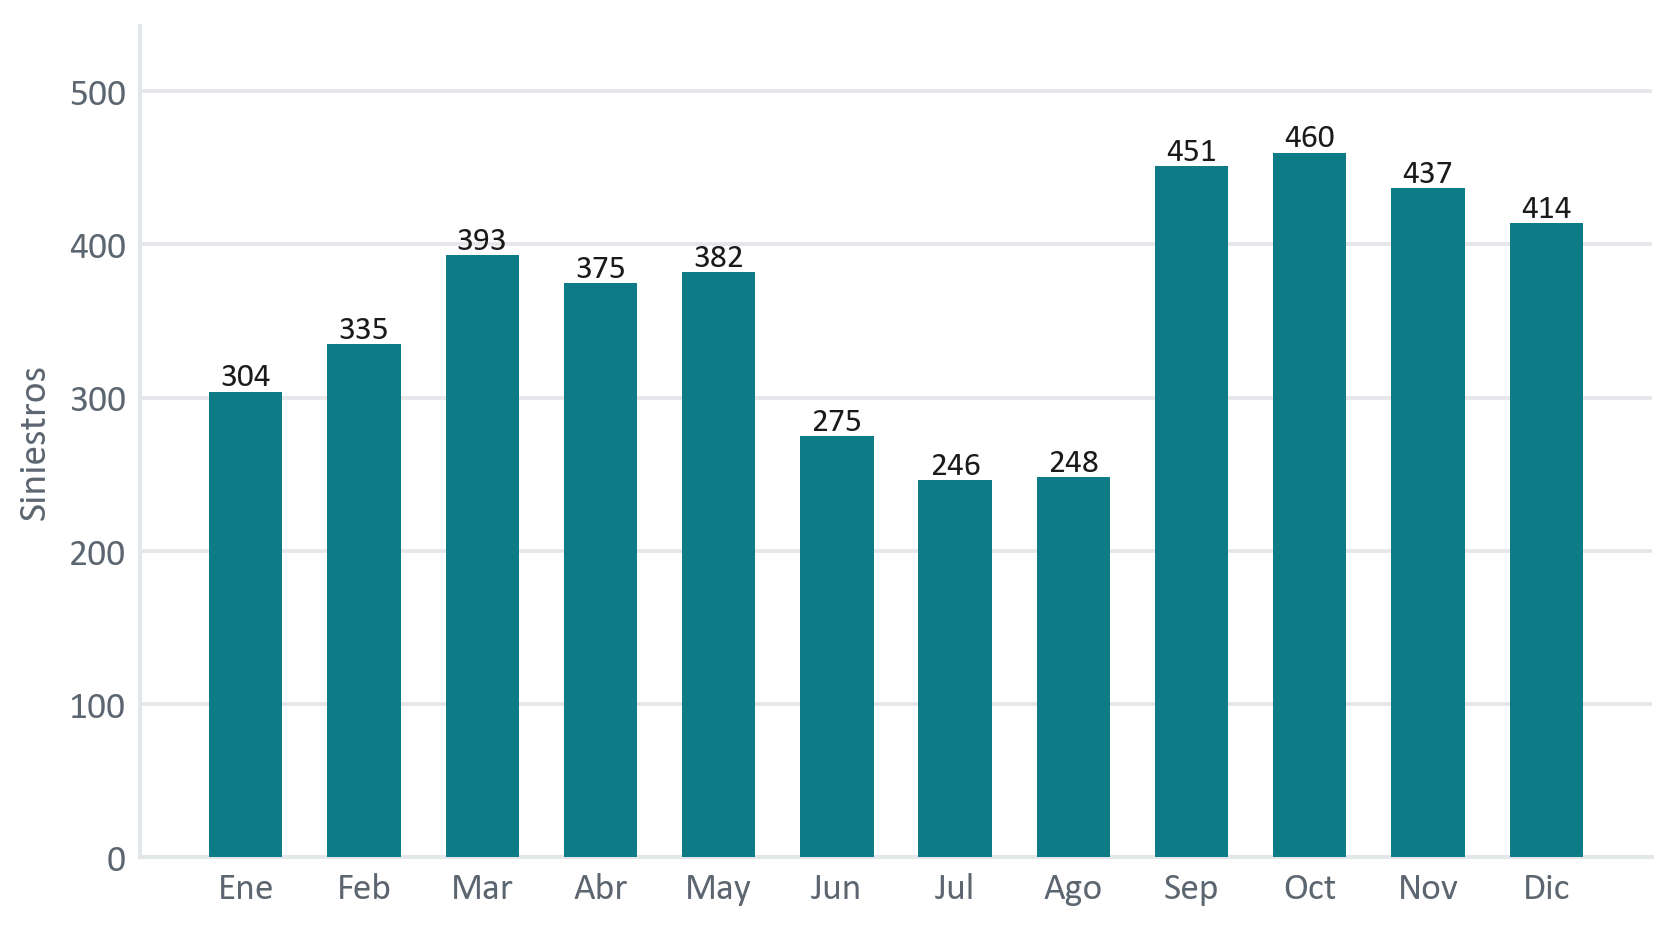
\includegraphics[width=0.92\linewidth]{imagenes/image2.png}
\caption{Distribución de siniestros viales por mes}
\label{fig:distribucion-de-siniestros-viales-por-me}
\notaflot{Frecuencia mensual acumulada de siniestros viales georreferenciados en la ciudad de Córdoba (n = 4320), julio 2022 -- junio 2024. El período de mayor concentración se ubica entre septiembre y diciembre, con un mínimo en julio y agosto. Julio computa únicamente 2023, y agosto 2022 y junio 2024 son meses parciales, por lo que esos tres meses acumulan menos años que el resto. \fuentepropia{} sobre la base de datos de la Unidad Judicial de Accidentología Vial.}
\end{figure}

\begin{figure}[htbp]
\centering
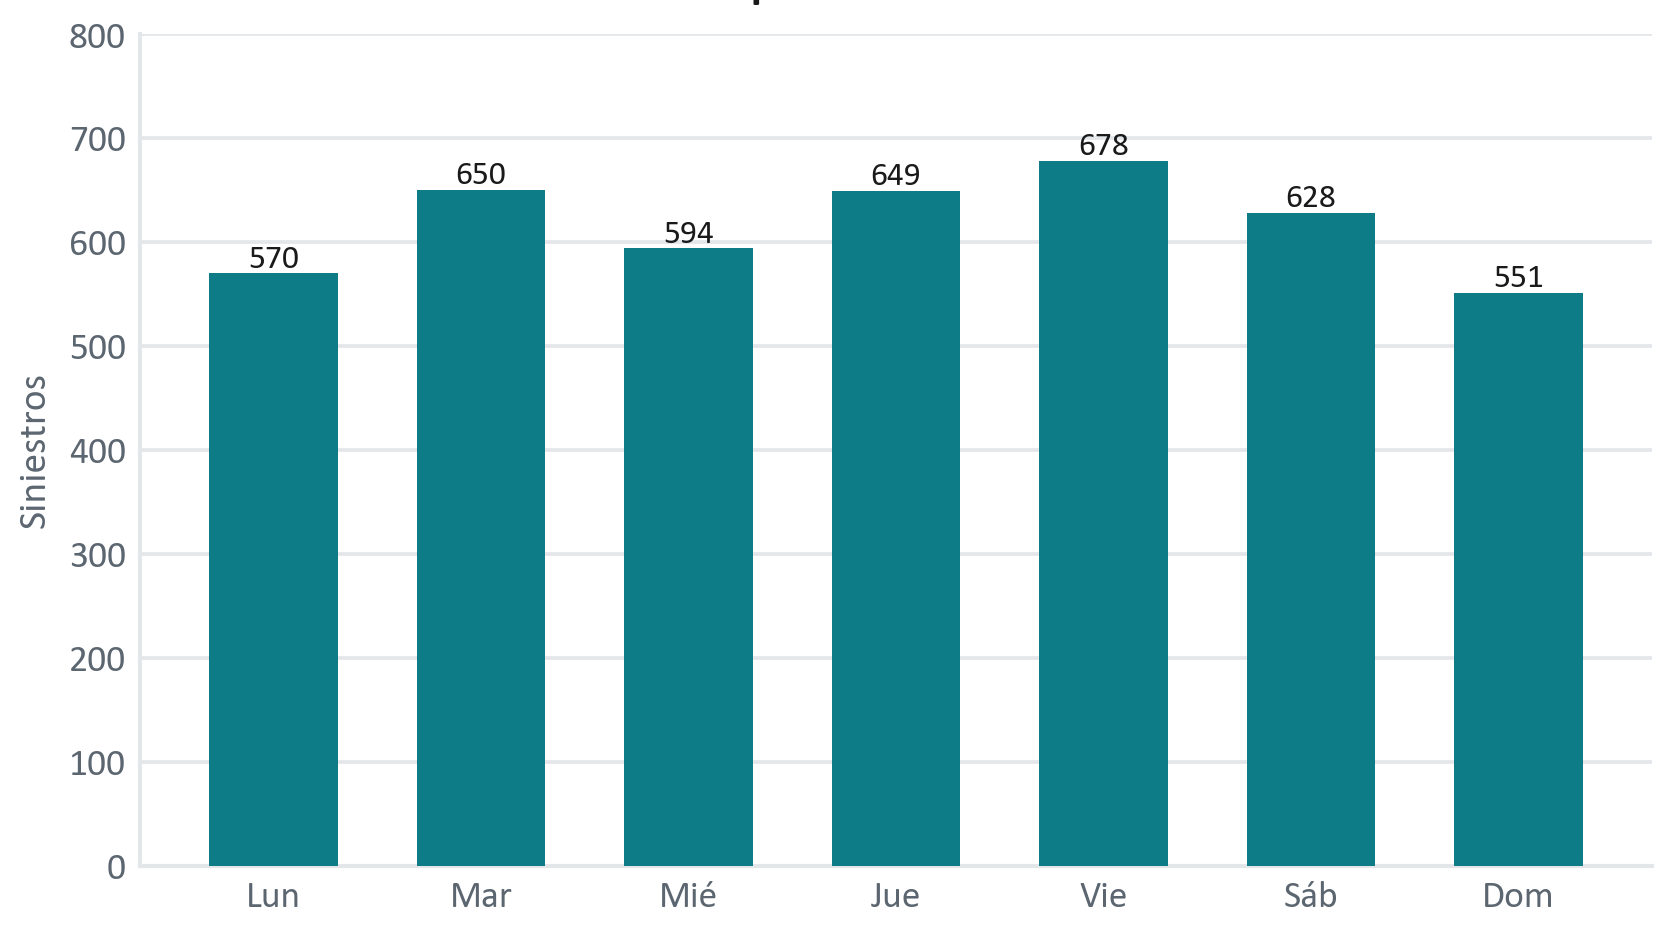
\includegraphics[width=0.92\linewidth]{imagenes/image1.png}
\caption{Distribución de siniestros viales por día de la semana}
\label{fig:distribucion-de-siniestros-viales-por-di}
\notaflot{Frecuencia de siniestros según día de la semana (n = 4320), julio 2022 -- junio 2024. La distribución es relativamente homogénea, con un máximo el viernes (678) y mínimos el domingo (551) y el lunes (570). \fuentepropia{}.}
\end{figure}

\begin{figure}[htbp]
\centering
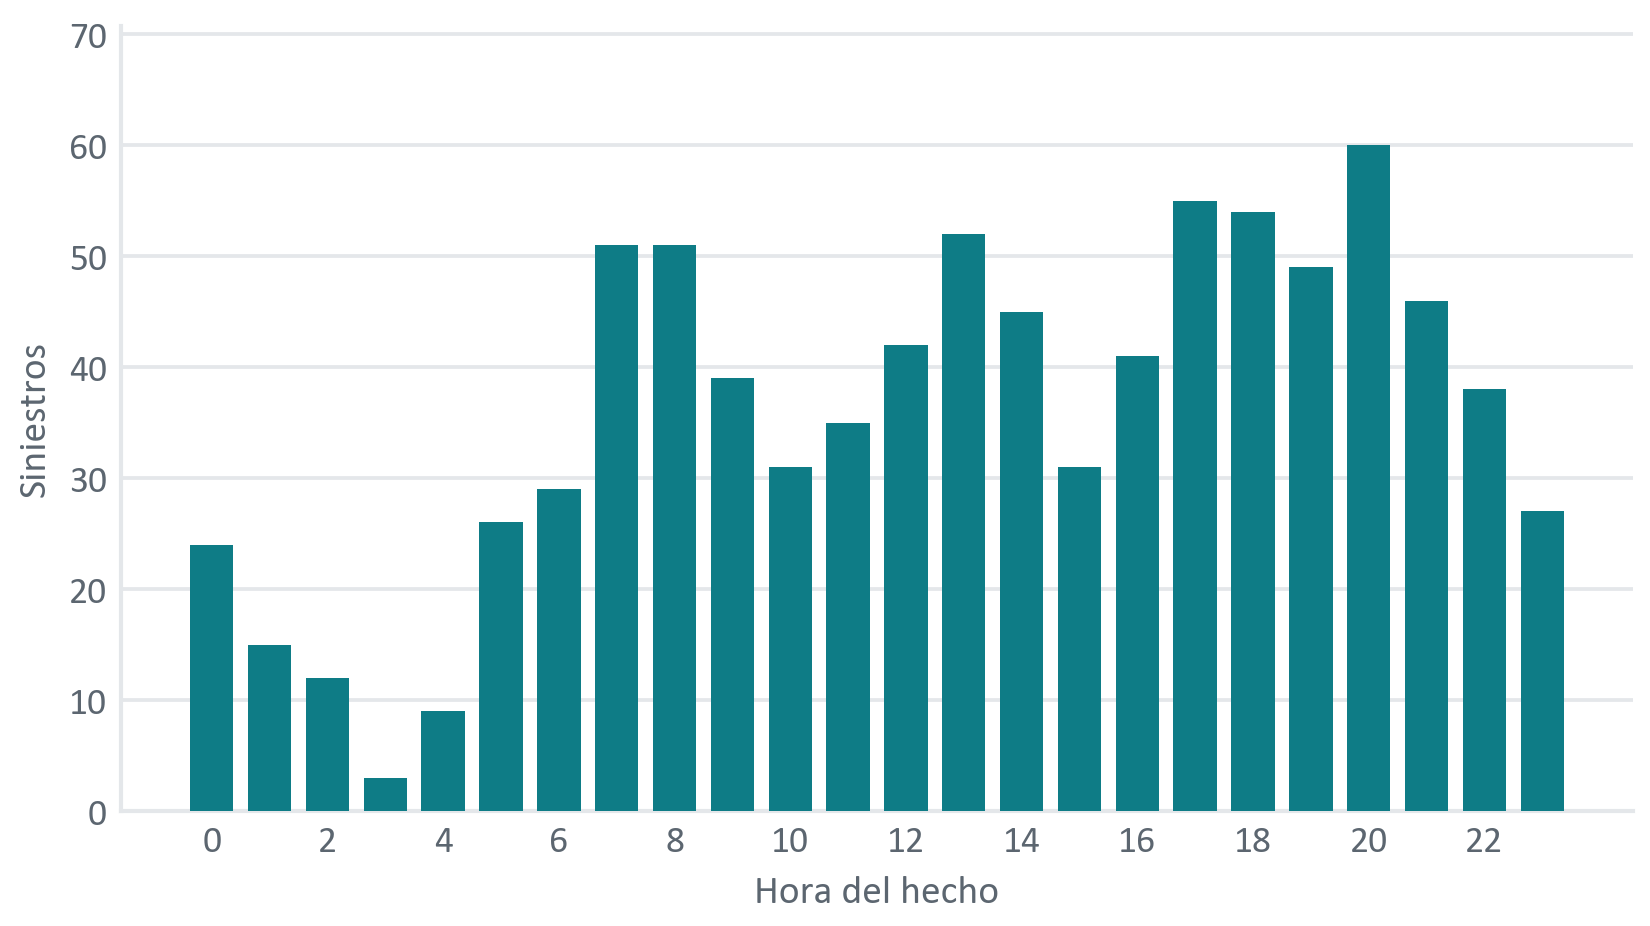
\includegraphics[width=0.92\linewidth]{imagenes/image6.png}
\caption{Siniestros viales por hora del día, año 2022}
\label{fig:siniestros-viales-por-hora-del-dia-ano-2}
\notaflot{Distribución horaria de los siniestros ocurridos durante 2022 (n = 865 registros con hora consignada; 23 casos sin dato, excluidos). Se identifican dos concentraciones asociadas a los desplazamientos cotidianos: una matutina (7 a 9 h) y otra vespertina, más prolongada e intensa (17 a 21 h), con el máximo absoluto a las 20 h. \fuentepropia{}.}
\end{figure}

\begin{figure}[htbp]
\centering
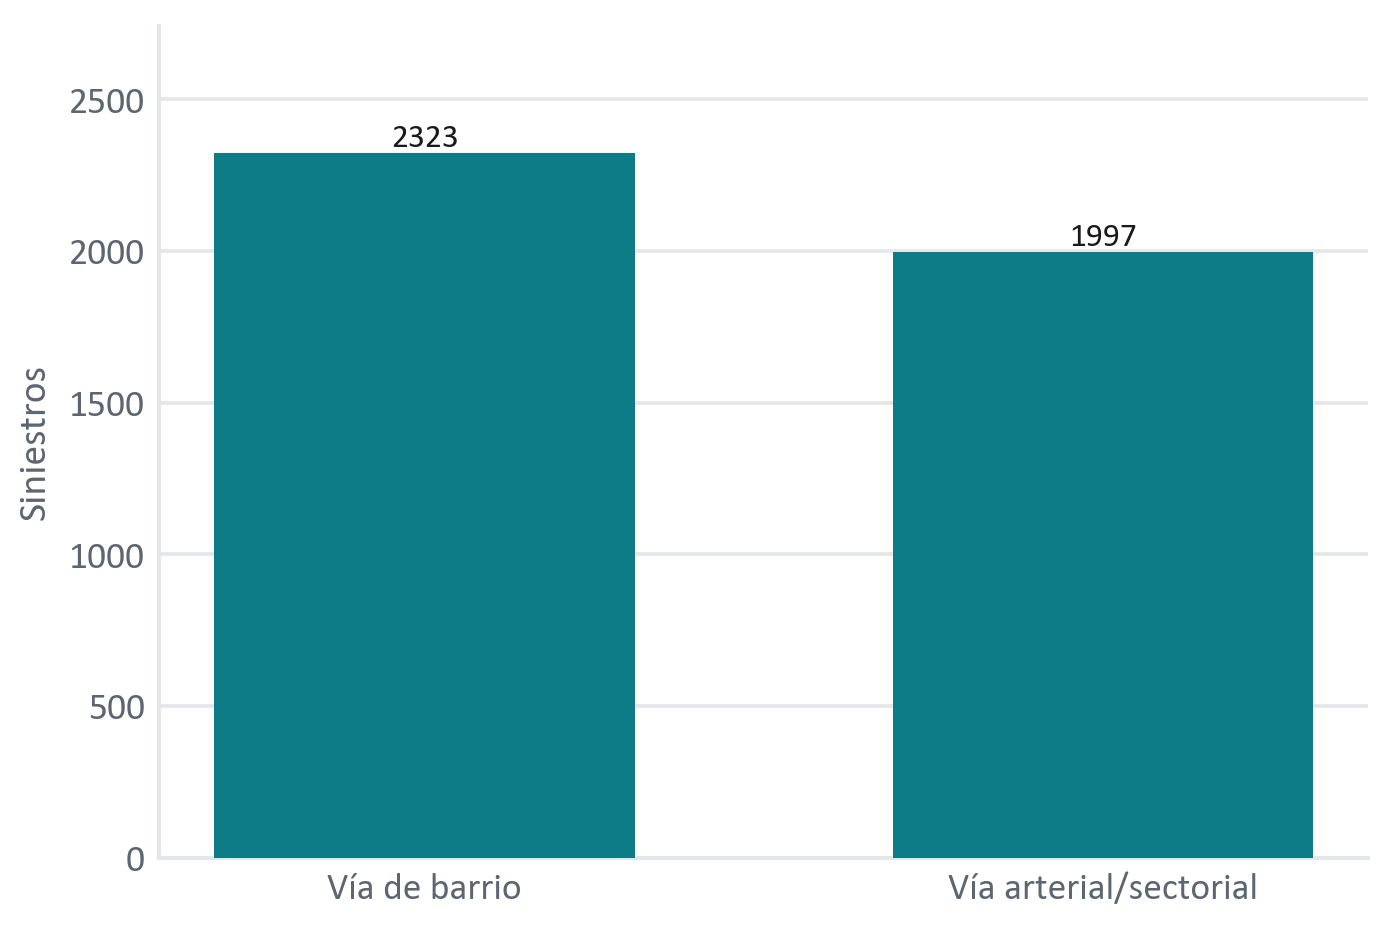
\includegraphics[width=0.78\linewidth]{imagenes/image3.png}
\caption{Distribución de siniestros viales por tipo de calle}
\label{fig:distribucion-de-siniestros-viales-por-ti}
\notaflot{Clasificación de los siniestros según jerarquía de la vía (n = 4320), julio 2022 -- junio 2024. Las vías de barrio concentran 2323 casos y las arteriales o sectoriales 1997, lo que muestra que el fenómeno no se restringe a los corredores principales. \fuentepropia{}.}
\end{figure}

\begin{figure}[htbp]
\centering
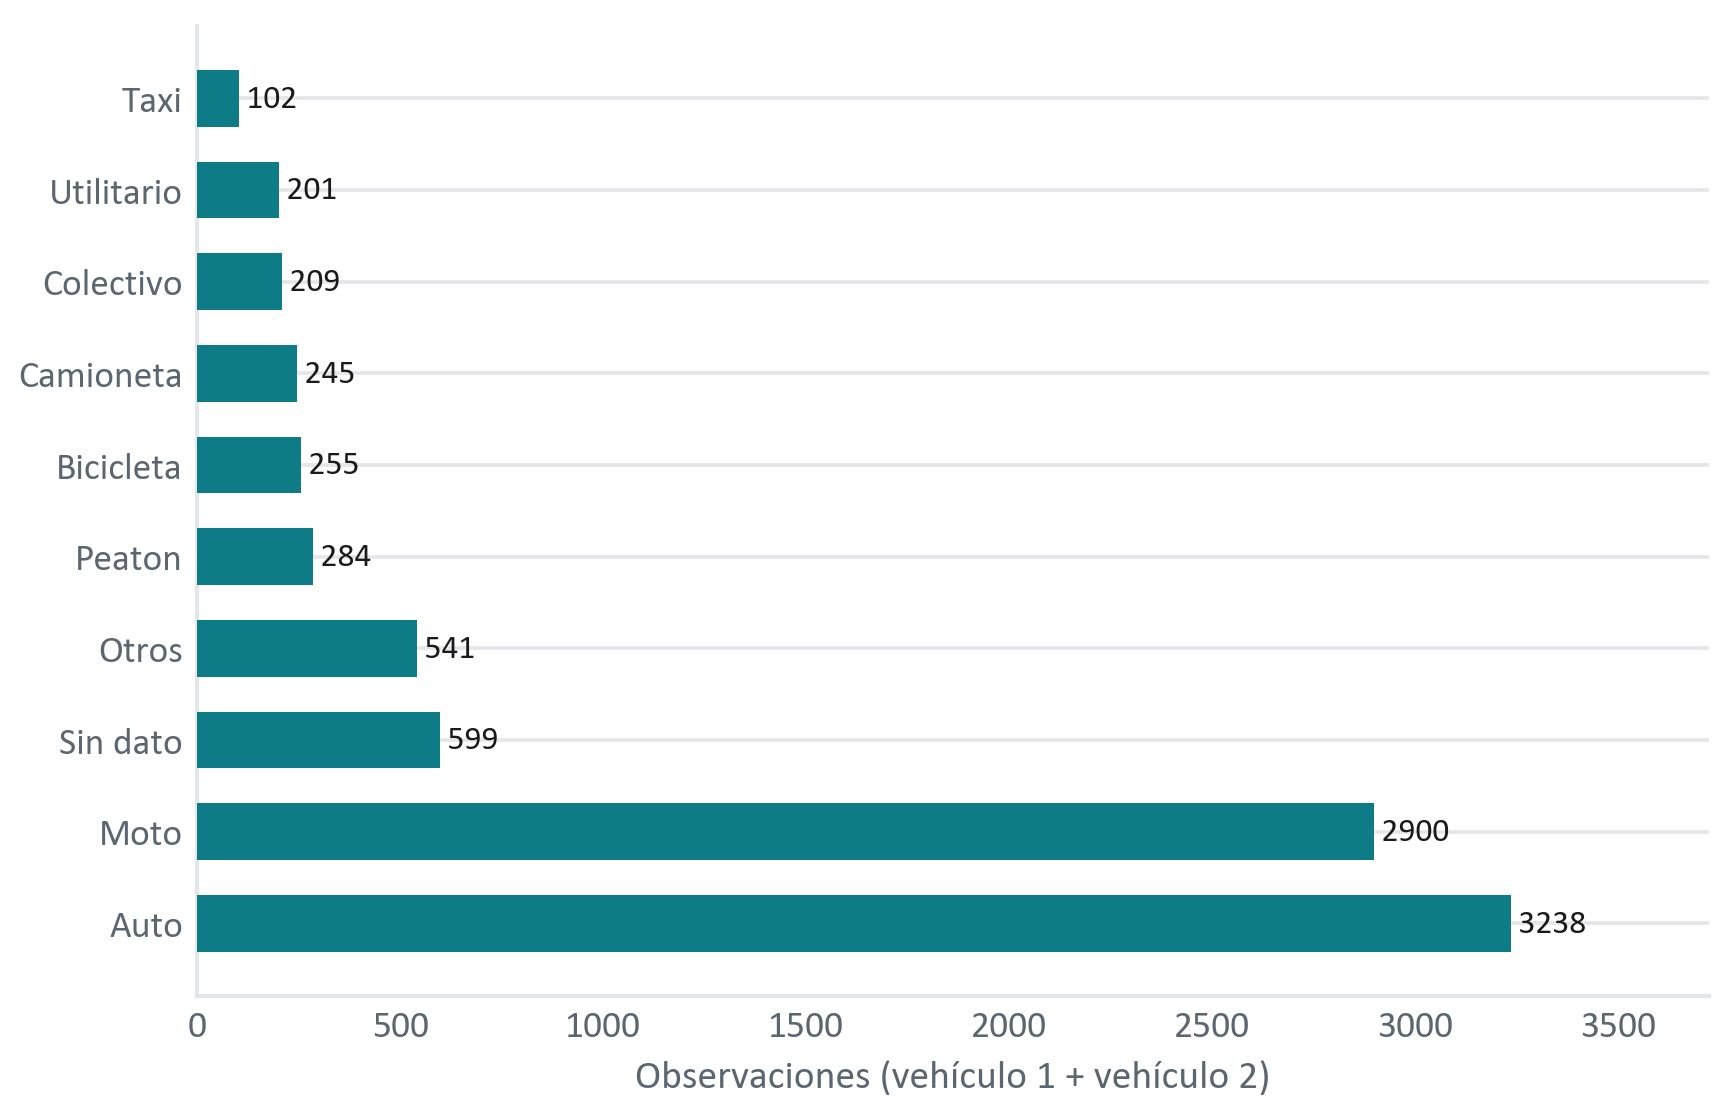
\includegraphics[width=0.81\linewidth]{imagenes/image16.png}
\caption{Distribución del tipo de vehículo o forma de desplazamiento}
\label{fig:distribucion-del-tipo-de-vehiculo-o-form}
\notaflot{Participaciones registradas en los 4320 siniestros (n = 8574 observaciones, correspondientes a vehículo 1 y vehículo 2). La unidad de conteo es la participación y no el siniestro, por lo que las categorías no son excluyentes entre sí. Autos (3238) y motos (2900) concentran la mayor parte de las observaciones. \fuentepropia{}.}
\end{figure}

\begin{figure}[htbp]
\centering
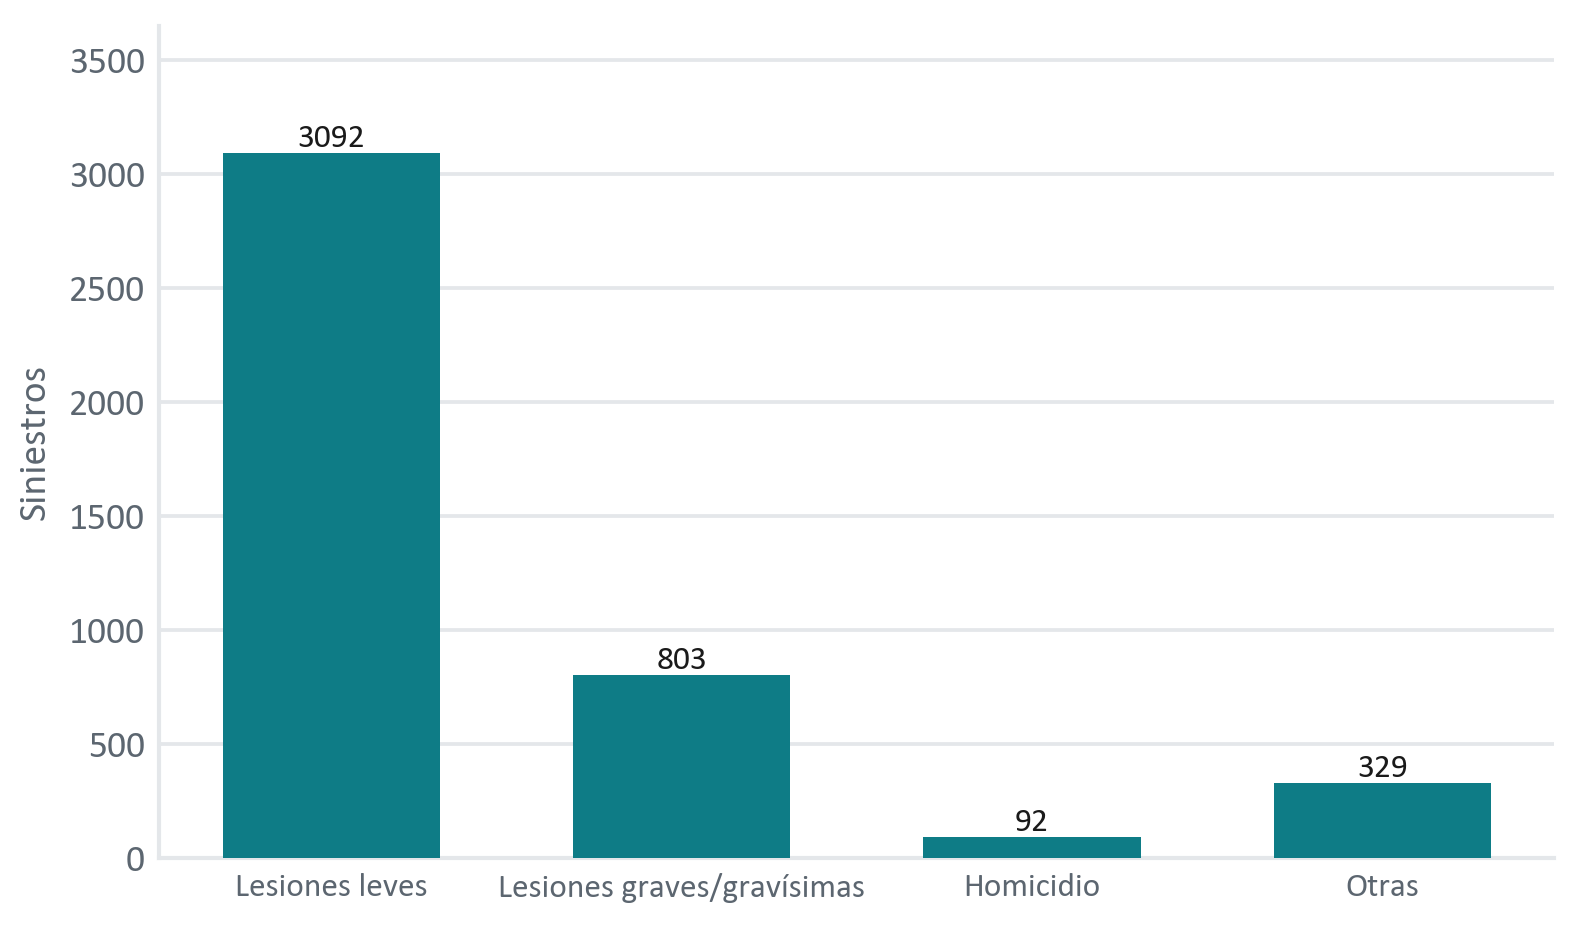
\includegraphics[width=0.89\linewidth]{imagenes/image5.png}
\caption{Distribución de siniestros viales según causa}
\label{fig:distribucion-de-siniestros-viales-segun-}
\notaflot{Clasificación de los siniestros según la carátula asignada en la causa judicial (n = 4316 casos clasificados; 4 sin clasificar, excluidos). Predominan las lesiones leves (3092), seguidas por lesiones graves o gravísimas (803), otras carátulas (329) y homicidio culposo (92). \fuentepropia{}.}
\end{figure}

\begin{figure}[htbp]
\centering
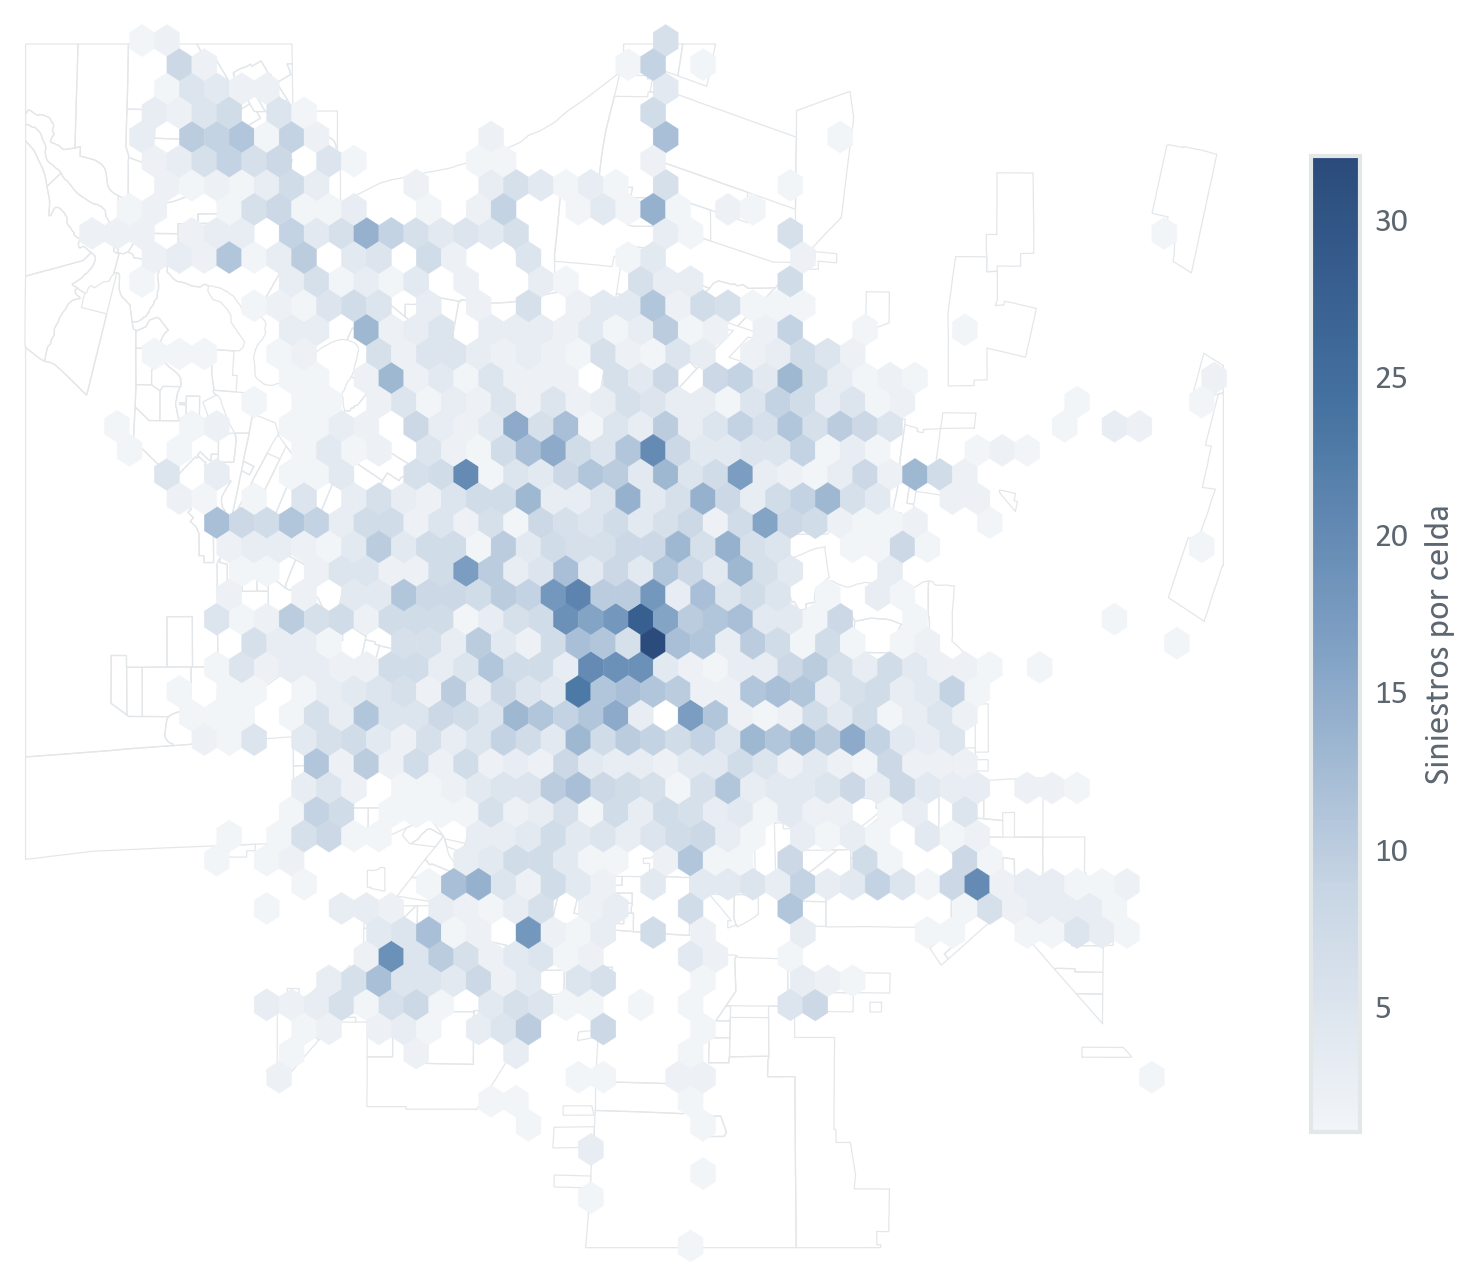
\includegraphics[width=0.92\linewidth]{imagenes/image8.png}
\caption{Mapa de calor de siniestros viales en la ciudad de Córdoba}
\label{fig:mapa-de-calor-de-siniestros-viales-en-la}
\notaflot{Densidad espacial de siniestros georreferenciados (n = 4320), julio 2022 -- junio 2024. La agregación se realiza por celda hexagonal de superficie constante y no por barrio; la silueta de los barrios se incluye solo como referencia visual. Se observa una concentración marcada en el área central y una difusión radial que sigue los principales corredores de acceso. \fuentepropia{}.}
\end{figure}

\section{Antecedentes Relevantes}\label{antecedentes-relevantes}

Una de las tareas que se realizó inicialmente fue la investigación y la búsqueda de antecedentes relevantes, es decir trabajos o publicaciones que fueran sobre el mismo tema o que traten aspectos del enfoque, los datos y las técnicas de aprendizaje automático que sean transferibles o aplicables al producto que se está desarrollando. En este sentido se analizaron principalmente 4 grupos de antecedentes, trabajos sobre accidentología vial de índole analítica o basados en el uso de datos, \eng{forecasting} para problemas similares como incidentes con ambulancias o incendios, sistemas de alerta temprana, ciudades inteligentes, entre otros.

Independientemente del campo de aplicación en el cual se aplicaban los modelos revisados se observaron 3 tipos de enfoques posibles que describen a grandes rasgos las capacidades y requerimientos que se necesitan para un problema con accidentes viales. El primero consiste en trabajar con GNNs, un tipo de arquitectura de redes neuronales basadas en grafos que aprenden patrones de una gran cantidad de datos y que, al procesarlas en sus nodos, permiten generalizar el comportamiento de un sistema. El segundo se basa en el uso de datos georreferenciados. Independientemente del modelo específico utilizado, permite no solo predecir cuándo existe un mayor riesgo de accidentes, sino también dónde es más probable que ocurran. El último consiste en construir una tabla a partir de los registros de accidentes, donde una vez tratada para adaptar el set de datos para que represente una serie temporal se aplican modelos basados en árboles para aprender en qué contexto se incrementa el riesgo de accidentes.

Respecto de los modelos basados en grafos, fueron descartados rápidamente por varios motivos. Si bien se consiguen muy buenos resultados, todos los casos revisados tenían varios órdenes de magnitud adicionales en cantidad de datos, los cuales no eran solamente de accidentes sino que incluyen gran cantidad de variables externas como datos demográficos, información georreferenciada, datos de seguros, criminología, etc. Otra de las motivaciones para desistir por lo menos al inicio en desarrollar un modelo de esta complejidad era el de comenzar con un modelo más simple y si se conseguía buena capacidad de generalización avanzar en estos tipos de sistemas.

El antecedente más significativo para este proyecto es \textcite{novello2022}, que consiste en resolver el mismo problema utilizando inteligencia artificial sólo que aplicado en Ciudad Autonoma de Buenos Aires. La metodología consiste en usar datos georreferenciados y retardos para intentar predecir las zonas con riesgo más elevado. Este enfoque puede categorizarse como sistemas impulsados por modelos espacio-temporales. Respecto de este antecedente, si bien se decidió reproducirlo, hay que tener en cuenta un componente que es determinante para el resultado del mismo, estamos hablando de la densidad de accidentes en el área de trabajo. Los datos para CABA totalizan \num{33234} registros de 29 características cada uno, distribuidos en 3,5 años y \qty{203}{\kilo\metre\squared}. Teniendo en cuenta la cantidad de registros para la Ciudad de Córdoba y el hecho de que tiene 2,8 veces más superficie (\qty{576}{\kilo\metre\squared}), la cantidad de accidentes por unidad de superficie es mucho menor por lo que el desempeño podría verse comprometido.

La última categoría mencionada es la de modelos tabulares basados en árboles. Generalmente requieren una menor cantidad de datos para alcanzar un buen desempeño que enfoques basados en redes neuronales profundas. Para esta metodología se encontró una cantidad considerable de trabajos, por lo que se deja como antecedente general el trabajo de \textcite{zheng2018} en su apartado sobre series temporales.

\section{Experimentación con Modelos}\label{experimentaciuxf3n-con-modelos}

\subsection{LightGBM para Intervalos de Predicción.}\label{lightgbm-para-intervalos-de-predicciuxf3n.}

El primer modelo que se probara consiste en entrenar un LightGBM con el objetivo de hacer un \eng{forecasting} sobre la cantidad de víctimas, la idea de implementar este modelo es que permite ver una línea temporal con la cantidad histórica de víctimas y a partir del punto actual se muestra una línea con el pronóstico esperado más los cuantiles \qty{10}{\percent} y \qty{90}{\percent} (correspondientes al mínimo y al maximo riesgo respectivamente).

Durante el proceso de entrenamiento se decidió crear nuevas variables y características intermedias para intentar mejorar al máximo el rendimiento del modelo, por mencionar algunos: \var{baseline\_60} como un promedio de los últimos 60 días y \var{promedio\_7dias} para los últimos 7 días. Otro aspecto que se debe destacar es que el modelo va a predecir varios bloques horarios de 6 horas, en concreto 28, es decir que el horizonte de predicción es de 7 días.

\begin{longtable}[]{@{}
>{\raggedright\arraybackslash}p{(\linewidth - 4\tabcolsep) * \real{0.3333}}
  >{\centering\arraybackslash}p{(\linewidth - 4\tabcolsep) * \real{0.3333}}
  >{\raggedright\arraybackslash}p{(\linewidth - 4\tabcolsep) * \real{0.3333}}@{}}
\caption{Métricas de rendimiento del modelo LightGBM híbrido L1}
\label{tab:metricas-de-rendimiento-del-modelo-final}\\
\toprule\noalign{}
\textbf{Métrica de Error} & \textbf{Valor} & \textbf{Interpretación} \\
\midrule\noalign{}
\endfirsthead
\toprule\noalign{}
\textbf{Métrica de Error} & \textbf{Valor} & \textbf{Interpretación} \\
\midrule\noalign{}
\endhead
\bottomrule\noalign{}
\endlastfoot
MAE (Mean Absolute Error) & 0,9741 & Medida de ajuste para datos de conteo (valores menores indican mejor ajuste). \\
MASE (Mean Absolute Scaled Error) & 0,1931 & Error Escala Estándar \\
& & \\
\end{longtable}

\notaflot{Métricas calculadas sobre el conjunto de test.}

\begin{figure}[htbp]
\centering
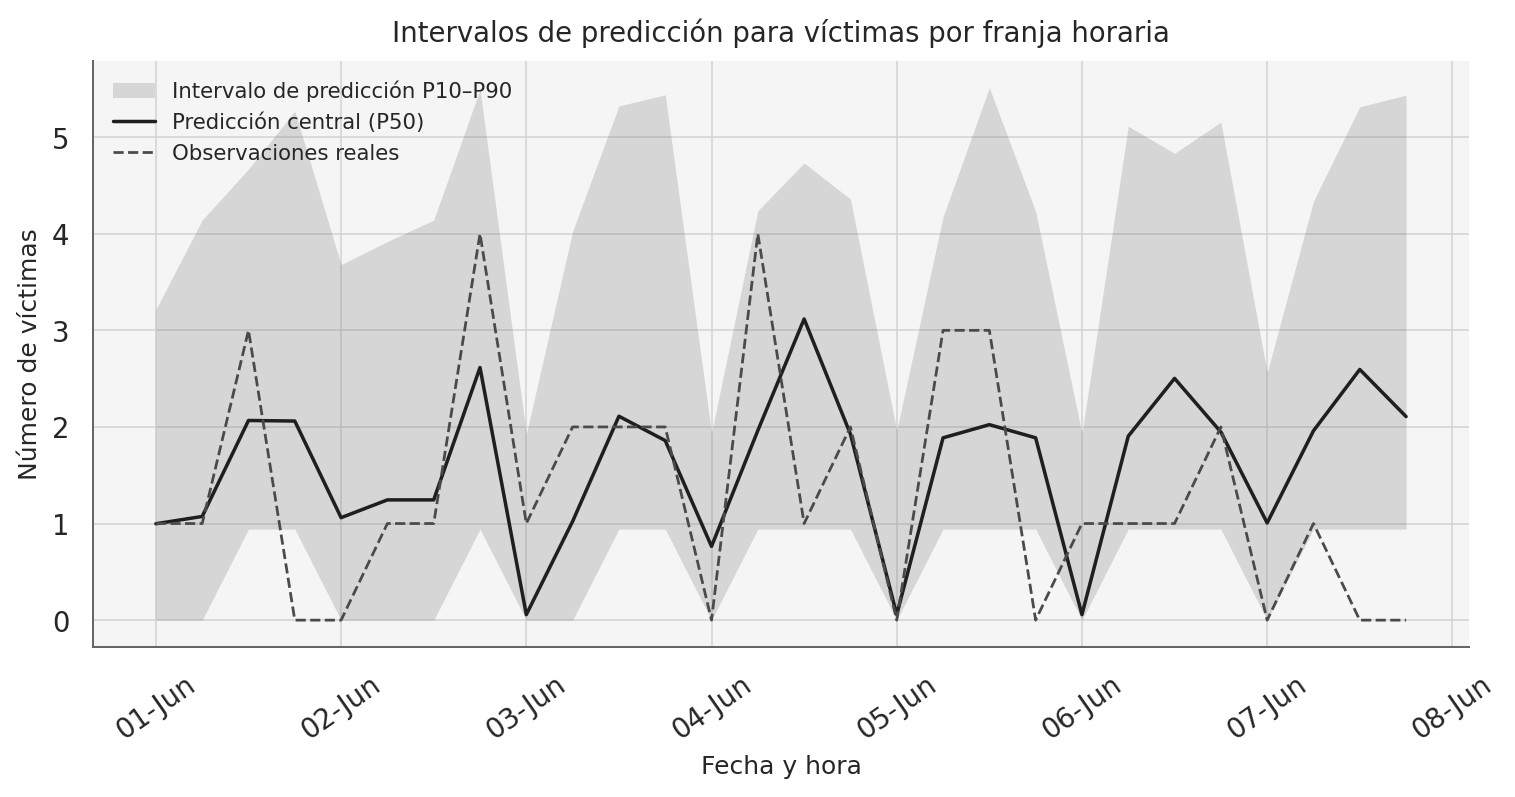
\includegraphics[width=\linewidth]{imagenes/image20.png}
\caption{Pronóstico con LightGBM: predicción central e intervalos P10--P90}
\label{fig:forecasting-lightgbm}
\notaflot{\fuentepropia{}.}
\end{figure}

En la \cref{fig:forecasting-lightgbm} se puede observar que si bien el modelo no se ajusta perfectamente a la realidad, logra identificar cuándo ocurrirán incrementos o descensos en la cantidad de víctimas en toda la ciudad. Este hallazgo sugiere que los datos le permiten a LightGBM aprender patrones de las tendencias de los mismos, y que enriquecerlos con más contexto puede mejorar el ajuste del \eng{forecasting}.

\subsection{Clasificador con Perceptrón Multicapa}\label{clasificador-con-perceptruxf3n-multicapa}

Se quiere probar si proponer una clasificación para los escenarios posibles le facilita a una red neuronal con un perceptrón multicapas alcanzar un buen desempeño. Para ello se generan 3 categorías diferentes a partir de las necesidades que tiene el MPF, las mismas son: Bajo para 2 víctimas o menos, Medio para hasta 4 víctimas y Alto a partir de 5 víctimas en un mismo bloque horario. Los resultados de este experimento se presentan en la \cref{tab:metricas-de-desempeno-multilayer-percept}:

\begin{longtable}[]{@{}
lcccc@{}}
\caption{Métricas de desempeño del clasificador de perceptrón multicapa}
\label{tab:metricas-de-desempeno-multilayer-percept}\\
\toprule\noalign{}
\endfirsthead
\toprule\noalign{}
\endhead
\bottomrule\noalign{}
\endlastfoot
& \textbf{Precisión} & \textbf{Recall} & \textbf{F1-Score} & \textbf{Support} \\
Alto & 0,0909 & 0,0125 & 0,0220 & 80 \\
Bajo & 0,5598 & 0,9035 & 0,6913 & 311 \\
Medio & 0,3469 & 0,0994 & 0,1545 & 171 \\
Accuracy & & & 0,5320 & 562 \\
Macro Avg & 0,3325 & 0,3385 & 0,2893 & 562 \\
Weighted Avg & 0,4283 & 0,5320 & 0,4327 & 562 \\
\end{longtable}

\notaflot{\fuentepropia{}.}

Con solo observar estas métricas podemos ver que el F1 ponderado de 0,4327 es bajo, indica que el desempeño general no es bueno, especialmente cuando se consideran las clases menos frecuentes. El Accuracy (Exactitud) de 0,5320 tampoco es una señal fuerte de buen rendimiento, porque el modelo puede ganar simplemente prediciendo mayoritariamente la clase ``bajo'' (Recall 0,9035). En conclusión se puede decir que segmentar el problema en 3 clases no es suficiente para generar un sistema de alerta temprana de utilidad, al menos en las condiciones actuales.

\subsection{XGBoost Regresor más Capa de Decisión Z-Score}\label{xgboost-regresor-muxe1s-capa-de-decisiuxf3n-z-score}

El problema recientemente mencionado obliga a replantear el enfoque con el cual va a trabajar el próximo modelo. Si generar tres categorías no es suficiente para alcanzar un buen rendimiento entonces se podría proponer un modelo que intente una regresión, es decir que prediga la cantidad exacta de víctimas que habrá y luego aplicar una capa de decisión posterior, la cual le indicará al usuario cual es el riesgo para ese contexto particular.

Para probar que tan bien puede funcionar esta propuesta se propone un XGBoost con 2227 datos para el conjunto de entrenamiento y 557 para el conjunto de prueba. La capa de decisión se ubica a la salida de dicho modelo, comparando la cantidad de víctimas predichas con un promedio histórico para ese contexto según el día y la franja horaria, es decir, si la predicción es de 5 víctimas para un viernes al mediodía entonces compara este valor con el promedio histórico de victimas para todos los viernes al mediodía del pasado. Luego mediante Z-Score ve que tan desviada está la predicción del promedio del pasado, según esta brecha realiza la categorización correspondiente en Bajo, Medio, Alto. Una ventaja que es destacable de este sistema es que permite que en el futuro se pueda calibrar la sensibilidad del modelo al variar los umbrales de Z. Los resultados se presentan en la \cref{tab:metricas-error-xgb-zscore}:

\begin{longtable}[]{@{}
>{\raggedright\arraybackslash}p{(\linewidth - 4\tabcolsep) * \real{0.3333}}
  >{\centering\arraybackslash}p{(\linewidth - 4\tabcolsep) * \real{0.3333}}
  >{\raggedright\arraybackslash}p{(\linewidth - 4\tabcolsep) * \real{0.3333}}@{}}
\caption{Métricas de error del XGBoost regresor con capa Z-Score}
\label{tab:metricas-error-xgb-zscore}\\
\toprule\noalign{}
\textbf{Métrica de Error} & \textbf{Valor} & \textbf{Interpretación} \\
\midrule\noalign{}
\endfirsthead
\toprule\noalign{}
\textbf{Métrica de Error} & \textbf{Valor} & \textbf{Interpretación} \\
\midrule\noalign{}
\endhead
\bottomrule\noalign{}
\endlastfoot
Poisson Deviance & 1,6627 & Medida de ajuste para datos de conteo (valores menores indican mejor ajuste). \\
MSE (Error Cuadrático Medio) & 1,2926 & Promedio de los errores cuadráticos entre el valor real y predicho. \\
RMSE (Raíz del Error Cuadrático Medio) & 1,137 & Desviación promedio del modelo. \\
\end{longtable}

\notaflot{Métricas calculadas sobre el conjunto de test independientemente del umbral de clasificación.}

\begin{figure}[htbp]
\centering
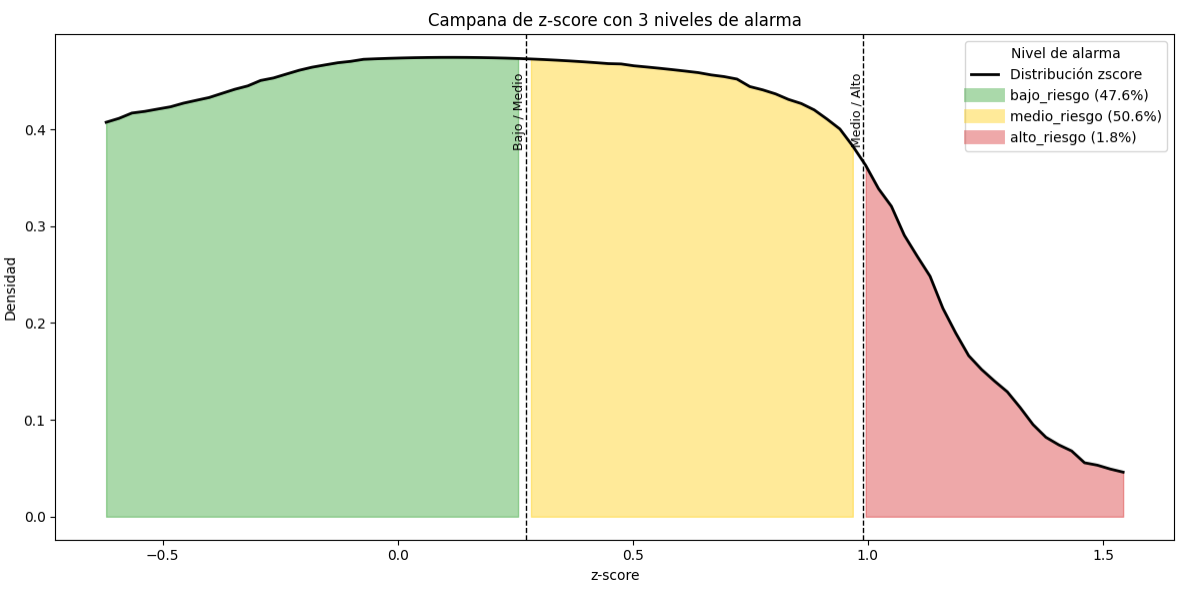
\includegraphics[width=\linewidth]{imagenes/image19.png}
\caption{Capa de decisión Z-Score y su distribución}
\label{fig:capa-de-decision-z-score-y-su-distribuci}
\notaflot{\fuentepropia{}.}
\end{figure}

Si bien las métricas no se pueden tomar como 100 por ciento satisfactorias, este modelo puede ser de mayor utilidad en comparación a los que se mencionaron hasta ahora, esto es debido a que si se exploran algunas nuevas variables que puedan contribuir a la mejoras de las métricas o si con el transcurso del tiempo estas mejoran debido al aumento en la cantidad de datos para entrenar, y se considera también el hecho de que tiene umbrales regulables que permiten ajustar las alertas a necesidad y criterio del usuario final, entonces puede considerarse seriamente para implementarlo en el MVP.

\subsection{Perceptrón Multicapa Binario con Capa de Decisión.}\label{perceptruxf3n-multicapa-binario-con-capa-de-decisiuxf3n.}

Considerando la metodología anterior, referida al uso de una capa de decisión posterior a la predicción del modelo, surge la pregunta entonces de qué pasaría con el desempeño del sistema en su conjunto si reemplazamos el XGBoost por un MLP. Se realizará entonces un experimento para comprobar cual de los dos modelos obtiene el mejor rendimiento para emitir las alertas.

En este caso es necesario recordar que las características del dataset son las mismas que en el XGBoost, esto es porque el objetivo es aislar el efecto del modelo para conocer exactamente cuánta es la contribución del MLP a la clasificación final. No obstante varía en cuanto a la naturaleza del atributo objetivo, el mismo es binario, es decir que el modelo tiene por salida una variable continua entre 0 y 1. Luego se procesan los quantiles para clasificar.

\begin{longtable}[]{@{}
>{\raggedright\arraybackslash}p{(\linewidth - 2\tabcolsep) * \real{0.3340}}
  >{\centering\arraybackslash}p{(\linewidth - 2\tabcolsep) * \real{0.3340}}@{}}
\caption{Métricas del perceptrón multicapa binario con capa de decisión}
\label{tab:resumen-de-metricas-del-modelo}\\
\toprule\noalign{}
\textbf{Métrica} & \textbf{Valor} \\
\midrule\noalign{}
\endfirsthead
\toprule\noalign{}
\textbf{Métrica} & \textbf{Valor} \\
\midrule\noalign{}
\endhead
\bottomrule\noalign{}
\endlastfoot
AUC-ROC & 0,6289 \\
Brier Score & 0,2053 \\
\end{longtable}

\notaflot{\fuentepropia{}.}

\subsection{XGBoost, Modelo Georreferenciado}\label{xgboost-modelo-georreferenciado}

Para desarrollar el modelo de forma tal que pase de ser solo temporal a espacio-temporal hay que realizar algunas consideraciones y tomar algunas decisiones importantes para adaptar esta solución a la ciudad de Córdoba.

La primera decisión que se tomó consistió en determinar de qué tamaño iban a ser las cuadrículas en la ciudad, inicialmente se propuso \qty{500}{\metre} por \qty{500}{\metre} en función del trabajo que se revisó \autocite{novello2022}, luego de un análisis estadístico se determinó que convenía hacer una cuadricula de \qty{1000}{\metre} por \qty{1000}{\metre} y si el modelo generaliza bien se podía reducir y evaluar los resultados.

Se tiene entonces la ciudad de Córdoba dividida en una cuadrícula como la mencionada, cada día tiene 4 bloques horarios de 6 horas, entonces cada combinación de área más rango horario es una fila del set de datos. Teniendo en cuenta que la ciudad tiene \qty{576}{\kilo\metre\squared} los registros totalizan \num{1472000} filas, de las cuales el \qty{0.28}{\percent} tienen accidentes. Este último número es la dificultad central del problema, un modelo que siempre predijera que no va a pasar nada acertaría el \qty{99.7}{\percent} de las veces. La \cref{fig:esquema-del-modelo-georreferenciado-impu} representa el proceso de entrenamiento.

\begin{figure}[htbp]
\centering
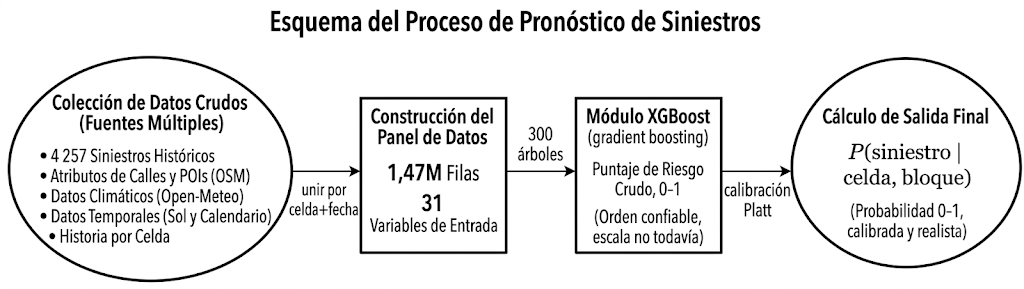
\includegraphics[width=\linewidth]{imagenes/image18.png}
\caption{Esquema del modelo georreferenciado impulsado por XGBoost}
\label{fig:esquema-del-modelo-georreferenciado-impu}
\notaflot{\fuentepropia{}.}
\end{figure}

Si bien este modelo obtuvo resultados modestos, promedio PR-AUC 0,0097 vs 0,0085 del promedio histórico; ROC-AUC 0,809 vs 0,778, permitió obtener información valiosa acerca del problema que se tendrá en cuenta cuando se desarrolle el modelo final. A forma de resumen podemos decir que la forma correcta de testear el modelo es usando Walk Forward, se debe evitar usar calibración isotónica cuando se tienen pocos casos positivos reemplazandola por Platt Scaling, y por último, se puede afirmar que el enfoque de trabajo georreferenciado funciona (el modelo ganó 5 veces ) y que si en el futuro se continúan recolectando datos tiene un gran potencial para crecer en cuanto a rendimiento.

En la sección siguiente se toman estas métricas como punto de partida, y se hace un resumen para sumarizar los hallazgos e indicios que se obtuvieron del proceso experimental.

\section{AutoGluon-TimeSeries}\label{autogluon-timeseries}

En la etapa final de exploración de modelos se desarrolló un proyecto en el Centro de Cómputos de Alto Desempeño de la Universidad Nacional de Córdoba (CCAD-UNC), el mismo consta de aplicar a los datos de este problema el pipeline de auto ML de AutoGluon-TimeSeries. Como se explicó en secciones anteriores este paso permite entrenar varios modelos simultáneamente para obtener una combinación óptima que maximice la performance.

\subsection{Configuración del Modelo AutoGluon y entrenamiento en CCAD}\label{configuraciuxf3n-del-modelo-auto-gluon-y-entrenamiento-en-ccad}

Se configuró el predictor de series temporales de AutoGluon (TimeSeries Predictor) para optimizar la métrica MASE sobre la variable objetivo en escala logarítmica (\var{victimas\_log}), ajustando los datos a una frecuencia de 6 horas con estacionalidad diaria ($m = 4$) y un horizonte de predicción de 14 días (56 pasos). Se definieron como covariables conocidas variables de calendario y contexto (\var{dia\_semana\_cat}, \var{es\_fin\_de\_semana}, mes y \var{tipomesESCOLAR}). El entrenamiento se ejecutó bajo el perfil \enquote{\var{high\_quality}} con un tiempo total de 12 horas, utilizando una estrategia de validación cruzada temporal (\eng{walk-forward}) de 4 ventanas consecutivas para garantizar una evaluación robusta sobre el histórico de datos.

\begin{longtable}[]{@{}
lcccc@{}}
\caption{Resultado del proceso de ensamble ponderado de AutoGluon}
\label{tab:resultado-del-proceso-de-ensamble-ponder}\\
\toprule\noalign{}
\textbf{Modelo} & \textbf{Score Test} & \textbf{Score Val} & \textbf{T Pred} & \textbf{T Ajuste} \\
\midrule\noalign{}
\endfirsthead
\toprule\noalign{}
\textbf{Modelo} & \textbf{Score Test} & \textbf{Score Val} & \textbf{T Pred} & \textbf{T Ajuste} \\
\midrule\noalign{}
\endhead
\bottomrule\noalign{}
\endlastfoot
Direct Tabular & -0,6983 & -0,8229 & 0,11 & 4,32 \\
DeepAR & -0,7011 & -0,8143 & 9,30 & 117,78 \\
Weighted Ensemble & -0,7116 & -0,7823 & 13,17 & 1,66 \\
Auto ETS & -0,7252 & -0,8077 & 4,25 & 72,69 \\
TFT & -0,7314 & -0,7911 & 0,40 & 416,63 \\
\end{longtable}

\notaflot{Los valores de Score corresponden a la métrica MASE invertida (multiplicada por -1), donde valores más cercanos a 0 indican mejor rendimiento. Los tiempos de predicción (T. Pred.) y ajuste (T. Ajuste) están expresados en segundos.}

Como se puede observar en estos resultados, el mejor desempeño lo tiene Direct Tabular, que en AutoGluon corresponde a modelos XGBoost o LightGBM configurados con ventanas deslizantes, lo que confirma las hipótesis de trabajos con las que se desarrollaron los modelos anteriores y se alinea con los antecedentes citados durante este proyecto.

\subsection{Resumen de Hallazgos en Experimentos}\label{resumen-de-hallazgos-en-experimentos}

En esta sección se analizarán los hallazgos de la etapa de experimentación teniendo en cuenta no sólo las métricas de los modelos, sino también expandiendo el análisis para contemplar otros criterios que no pueden obviarse si se quiere obtener una solución que se ajuste a las necesidades del usuario y su contexto.

El primer aspecto a tratar es cómo se va a predecir la variable objetivo, habiéndo se trabajado en dos posibilidades, las regresiones para valores continuos en la cantidad de víctimas y las clasificaciones tanto binarias como en diferentes categorías. Los hallazgos sugieren que a todos los modelos entrenados les cuesta identificar momentos de bajo riesgo independientemente de cómo se le pida la salida a los mismos, tomando el caso por ejemplo del MLP en clasificación binaria con una curva AUC-ROC de 0,6289 o el caso de XGBoost con Recall de 0,39 (identificó sólo el \qty{39}{\percent} de los momentos en donde no hubo accidentes viales) en momentos seguros y 0,87 para momentos críticos (este modelo se desarrolla con más profundidad en el siguiente apartado). De los demás experimentos realizados se puede dejar como observación que el LightGBM que se configuró para mostrar la línea de predicción más intervalos P10 y P90 logra identificar mejor los momentos seguros que las otras variantes.

El siguiente hallazgo puede resumirse en que si se compara el desempeño de los modelos clasificadores contra los regresores resulta notablemente mejor hacer un sistema híbrido compuesto por un modelo regresor y una capa de decisión adicional que clasifique el riesgo luego de hacer la predicción. En este sentido se destaca el XGBoost Regresor con capa de decisión Z-Score en comparación por ejemplo con el MLP que clasifica directamente en Alto, Medio y Bajo que solo tiene un desempeño aceptable en una de sus clases.

A lo largo de todo el proceso de experimentación se pudo confirmar mediante la realización de entrenamientos con múltiples modelos y búsqueda por grilla de hiperparámetros que el fenómeno puede explicarse principalmente por el comportamiento histórico de la cantidad de víctimas y algunas variables representativas del dia de la semana y el rango horario que se está observando. Es decir que no se observaron contribuciones significativas a la capacidad predictiva de variables como la temperatura, la presión, el periodo escolar y otras variables. Este aspecto se encuentra mejor explicado en la sección de resultados del modelo de línea de base.

Respecto del modelo de línea de base, se optó por seleccionar XGBoost configurado para regresión de Poisson, el motivo de esto es obtener un modelo que pueda ser usado de base de comparación para medir la evolución de futuros reentrenamientos, mejoras, adaptaciones, y también de cómo evoluciona la capacidad de predicción cuando se incorporen nuevos datos. Si bien este modelo termina por clasificar de forma binaria la ocurrencia de un siniestro, solo lo hace definiendo un umbral fijo predefinido. Esta decisión no se tomó arbitrariamente, es necesario usar de línea de base la capacidad predictiva propia del modelo, aislandolo de los efectos del uso posterior de capas de decisión como las Z-Score.

\section{Pipeline del Modelo de Línea Base (Baseline)}\label{pipeline-del-modelo-de-luxednea-base-baseline}

En esta instancia se explicará cómo se generó el modelo de línea de base para este proyecto, usualmente se trabaja con un modelo que tiene una complejidad relativamente baja respecto de otras técnicas, con el objetivo de experimentar rápidamente y testear diferentes hipótesis que permitan confirmar si los datos tienen la calidad y cantidad suficiente \autocite{zheng2018} como para que un determinado modelo pueda adquirir una capacidad de generalización útil para el fin en cuestión. En este caso se decidió comenzar con un árbol de decisión XGBoost por el hecho de que permite recuperar información acerca de la importancia de cada variable para generar la predicción, esto es un insumo fundamental para realizar uno de los procesos fundamentales del Machine Learning que es denominado ingeniería de características y que es el que permite comprender mejor la naturaleza del fenómeno estudiado.

La estructura definida en el apartado anterior es de gran valor a la hora de comprender el problema que se quiere abordar, es lo suficientemente específica, amplia en el sentido de contener muchas características y adecuado para aplicar modelos de distintos tipos como pueden ser clasificadores para buscar patrones en grupos o modelos de analítica descriptiva más clásicos que permitan obtener información valiosa. Esto es posible porque el dataset contiene mucha información que caracteriza cada hecho en particular, como por ejemplo el tipo de vehículo involucrado, datos sobre las personas involucradas, distancia al semáforo más próximo, datos de referenciación geográfica, entre otros. Sin embargo, la forma en la que esta información está estructurada no es útil para la realización de \eng{forecasting} para un sistema que pretende anticipar en una ventana de tiempo la cantidad de víctimas o lesionados que pudiera haber, esto es por un motivo trivial, cuando trabaja con series temporales se utiliza información disponible en el momento o que se tiene del pasado para poder realizar la predicción, pero en todos los casos tiene que ser información disponible antes del suceso que se quiere pronosticar. El formato en el que se encuentran los datos actuales es denominado Tabla de Hechos, y consiste básicamente en que cada fila es un registro de un hecho puntual en un determinado momento, es decir que de manera general contiene la fecha y hora, y en las columnas consecutivas información relevante del evento.

Uno de los principales aspectos que debió reformularse al inicio del proyecto es el derivado de la propia naturaleza de la tabla de hechos, la cual no registra el tiempo de manera continua, es decir, que los días en los que no hay accidentes no se tiene información, esto es especialmente relevante para diseñar una alerta temprana dado que es de vital importancia saber bajo qué condiciones no ocurren accidentes. Para solucionar este problema se optó por dividir un cada día en bloques de 6 horas, de manera tal que la cantidad de accidentes que corresponden a un mismo bloque horario se suman para representar el riesgo de tal, cuando no existan accidentes el bloque contiene un cero para indicarle al modelo que no pasó nada. Las demás variables son agregadas de igual manera según criterios convenientes de manera tal que representen lo mejor posible a cada bloque, por ejemplo para la temperatura se toma el promedio durante las 6 horas correspondientes. Es importante destacar que la decisión de dividir el día en 4 bloques de 6 horas cada uno no es arbitraria sino que fue tomada en base a experiencias del personal del ministerio público fiscal y consultada con distintos especialistas pertenecientes a LIDeSIA.

\begin{figure}[htbp]
\centering
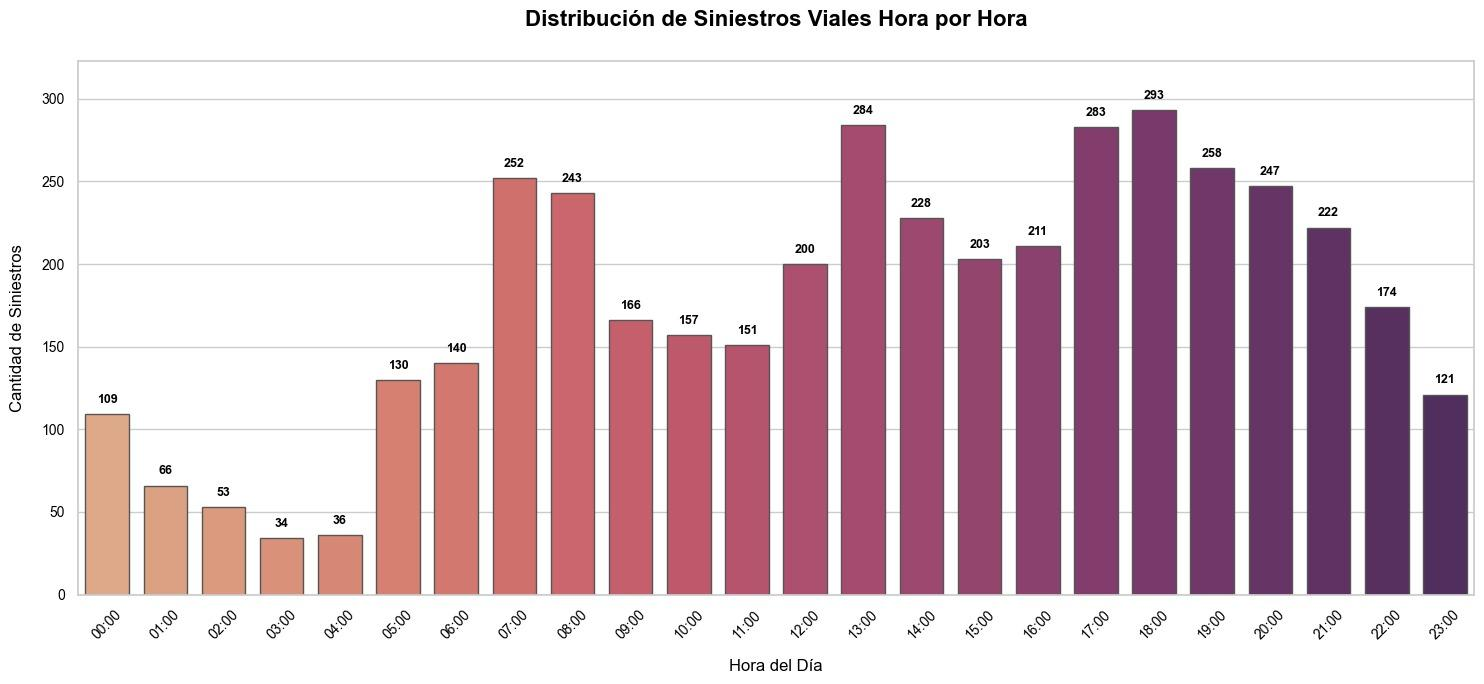
\includegraphics[width=\linewidth]{imagenes/image23.jpg}
\caption{Distribución del total de accidentes por hora del día}
\label{fig:distribucion-del-total-de-accidentes-por}
\notaflot{\fuentepropia{}, a partir de los datos provistos por el Ministerio Público Fiscal.}
\end{figure}

Continuando con las estrategias implementadas para poder aplicar un modelo XGBoost (Extreme Gradient Boosting) se explicará cómo se modificó el set de datos para cambiar la forma en que representa la información. El objetivo final es que cada registro ordenado cronológicamente contenga información dividida en tres partes, datos del pasado, datos del presente, y la cantidad de accidentes que hubo en ese contexto.

Para esto se utilizará un enfoque llamado Formulación Autorregresiva Supervisada que consiste en traer al presente información del pasado por medio de retardos (Lags) y sumarlo a los datos del presente para generar el contexto que explique la cantidad de víctimas que hubo en ese momento. Un ejemplo de esto puede ser la propia cantidad de víctimas de un bloque horario de 6 horas, por ejemplo, para un dia viernes por la tarde reconstruirse información del pasado trayendo al presente el promedio de víctimas de la última semana, las víctimas del viernes anterior, las víctimas de las últimas 12 horas e infinidad de combinaciones posibles que se pueden generar con esta y otras variables como las climáticas por ejemplo. Siguiendo este método, para generar un registro basta con crear un algoritmo que se desplace pasos hacia atrás en el tiempo, agregue la información que se requiere y la inscriba en el registro actual.

Nótese de esta manera que lo que representan los datos cambió totalmente, antes se tenía una serie de registros que ubican cada accidente en particular de manera irregular y con información que caracteriza el hecho en sí, ahora en cambio, se tiene un set de datos que representa el estado de un sistema (Tránsito de la Ciudad de Córdoba) definido por una serie de características las cuales al variar en el tiempo generar incrementos o decrementos del riesgo de accidente vial. Una vez que el modelo sea entrenado, el mismo aprenderá a detectar los patrones que generan una subida en la cantidad de víctimas registradas, así como qué combinación de variables hace que el riesgo del sistema de tránsito permanezca bajo.

\begin{figure}[htbp]
\centering
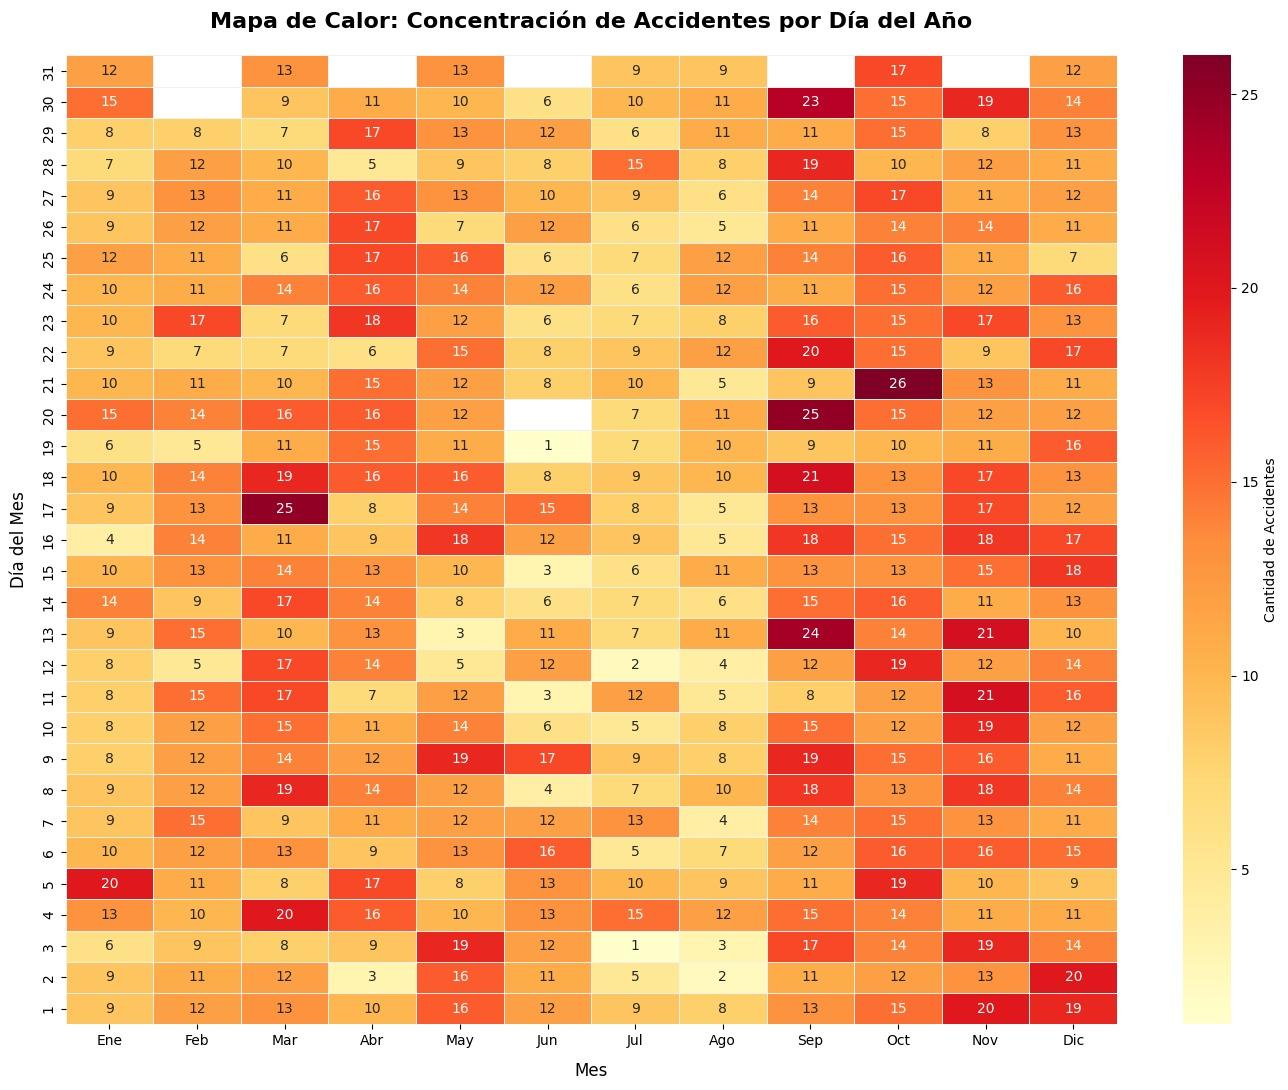
\includegraphics[width=\linewidth]{imagenes/image24.jpg}
\caption{Concentración de accidentes por día del año}
\label{fig:mapa-calor-dia-anio}
\notaflot{\fuentepropia{}.}
\end{figure}

\subsection{Definición de la estructura de Ventanas Deslizantes}\label{definiciuxf3n-de-la-estructura-de-ventanas-deslizantes}

En este punto se comienza definiendo la variable objetivo para el entrenamiento de Machine Learning, la variable objetivo es la que el modelo intenta predecir a partir de las demás características o features que aporta el set de datos. Para este caso se definió una variable denominada en el dataset como \var{TARGET\_CRITICO} la cual es de naturaleza binaria, es decir que toma el valor de 1 cuando existe al menos una víctima de accidente vial y 0 cuando no pasó nada. La relación con el formato de ventana deslizante consiste en que esta variable será la que permite calcular los retardos que se mencionan más adelante.

Por otro lado se tienen las variables relacionadas a la dimensión del tiempo, como por ejemplo el día está codificado con un 1 para el Lunes, 2 para el Martes y así sucesivamente. Análogamente se categorizaron las franjas horarias en este caso 1 significa la franja que va desde las 00:00 horas hasta las 06:00 horas, el 2 es el bloque contiguo, lo mismo ocurre con la variable mes del año en cuestión. En las variables que refieren al tiempo puede ocurrir un problema dependiendo el modelo que se esté utilizando, este radica en el hecho de que el mismo no entiende que el tiempo es cíclico en el sentido que para el algoritmo el lunes está a una distancia de 6 respecto al domingo, cuando en realidad también los separa una distancia de 1. En este caso tenemos la posibilidad de aplicar una transformación seno coseno a cada una de estas variables solucionando el inconveniente anterior. En el caso de árboles de decisión su uso no es del todo recomendable porque puede generar inconvenientes, pero es necesario aclararlo por si en el modelo definitivo se deciden usar modelos complementarios como el Perceptrón Multicapa por ejemplo.

Si se tiene presente la estrategia de las ventanas deslizantes para traer de forma autorregresiva información del pasado al presente para predecir el futuro, es razonable plantearse que no solo una agregación de las últimas víctimas que hubo en horas pasadas puede ser suficiente para poder hacer un \eng{forecasting} con algún grado de precisión, en cambio conviene generar adecuadamente un tipo de variable que indique tendencias o inercia, esto es por que se sospecha que si existe alguna tendencia al alza en el corto plazo es razonable que en el futuro próximo existan más accidentes. Este es el caso por ejemplo de la variable \var{tendencia\_corto\_victimas} que representa la diferencia entre las víctimas de las últimas 6 horas y las víctimas de las últimas 24 horas, este principio se extiende a variables de clima, de cantidad de lesionados y demás datos correspondientes. La \cref{tab:estructura-y-tipos-de-datos-del-conjunto} detalla la configuración final del conjunto de datos.

\begin{longtable}[]{@{}rll@{}}
\caption{Estructura y tipos de datos del conjunto de entrenamiento}
\label{tab:estructura-y-tipos-de-datos-del-conjunto}\\
\toprule\noalign{}
\textbf{\#} & \textbf{Variable} & \textbf{Tipo de dato} \\
\midrule\noalign{}
\endfirsthead
\toprule\noalign{}
\textbf{\#} & \textbf{Variable} & \textbf{Tipo de dato} \\
\midrule\noalign{}
\endhead
\bottomrule\noalign{}
\endlastfoot
0 & \var{hora\_sin} & float64 \\
1 & \var{hora\_cos} & float64 \\
2 & \var{dia\_sin} & float64 \\
3 & \var{dia\_cos} & float64 \\
4 & \var{mes\_sin} & float64 \\
5 & \var{mes\_cos} & float64 \\
6 & \var{es\_fin\_de\_semana} & float64 \\
7 & tavg & float64 \\
8 & pres & float64 \\
9 & \var{cambio\_presion} & float64 \\
10 & \var{cambio\_temperatura} & float64 \\
11 & \var{victimas\_lag\_1} & float64 \\
12 & \var{lesiones\_lag\_1} & float64 \\
13 & \var{victimas\_lag\_4} & float64 \\
14 & \var{promedio\_victimas\_24h} & float64 \\
15 & \var{tendencia\_corto\_victimas} & float64 \\
16 & \var{aceleracion\_riesgo} & float64 \\
17 & \var{victimas\_mismo\_momento\_6d} & float64 \\
18 & \var{lesiones\_mismo\_momento\_6d} & float64 \\
19 & \var{tipomesESCOLAR\_2} & float64 \\
20 & \var{TARGET\_CRITICO} & int64 \\
\end{longtable}

\notaflot{El conjunto de datos consta de 2784 entradas (índice 0 a 2783) con un total de 21 variables, de las cuales 20 son de tipo continuo (float64) y 1 entera (int64).}

Un detalle importante a destacar sobre el proceso de ingeniería de variables es que si bien se detalla el resultado final, eso no significa que las variables propuestas fueran seleccionadas arbitrariamente, por el contrario, este proceso es uno de los más extensos en tiempo y recursos que tiene cualquier Pipeline de Machine Learning junto con el tratamiento inicial de los datos crudos. Naturalmente este proyecto que aquí se presenta no fue la excepción y luego de entrenar varios modelos en simultáneo, analizar sus métricas, ventajas y desventajas se llegó al óptimo que se describió recientemente.

\subsection{Entrenamiento del modelo XGBoost}\label{entrenamiento-del-modelo-xg-boosting}

A continuación se describe la estructura y las configuraciones de los hiper parámetros con los cuales se entrenó el modelo XGBoost, además de algunas precisiones sobre cómo es que funciona este modelo aplicado a un sistema de alerta temprana (SAT).

Como se mencionó previamente, la variable objetivo de este modelo es un atributo de tipo binario que toma el valor de uno cuando se tiene al menos una víctima de accidente vial y cero en el momento que no hay víctimas por esta causa. La estrategia seleccionada para esta ocasión consiste en configurar el modelo como un regresor de Poisson, esto no es algo menor dado que también sería posible hacer un clasificador binario que prediga directamente 0 o 1 según corresponda (este experimento se realizó, no obteniendo un buen desempeño). Un regresor de Poisson tendrá como salida al final del modelo un valor continuo entre cero y uno, el cual representa la tasa o expectativa de que ocurra al menos un accidente.

Un método muy extendido en el campo de la ciencia de datos y el machine learning es el uso de la búsqueda por grillas a la hora de encontrar los mejores hiper parámetros (configuraciones previas al entrenamiento que influyen en la capacidad de generalización del modelo). Esto quiere decir que se realizan varios entrenamientos con distintas configuraciones para lograr encontrar el modelo con mejores resultados. La \cref{tab:hiperparametros-optimizados-del-modelo} resume los resultados preliminares.

\begin{longtable}[]{@{}
>{\raggedright\arraybackslash}p{(\linewidth - 2\tabcolsep) * \real{0.3340}}
  >{\centering\arraybackslash}p{(\linewidth - 2\tabcolsep) * \real{0.3340}}@{}}
\caption{Hiperparámetros optimizados del modelo}
\label{tab:hiperparametros-optimizados-del-modelo}\\
\toprule\noalign{}
\textbf{Hiperparámetro} & \textbf{Valor} \\
\midrule\noalign{}
\endfirsthead
\toprule\noalign{}
\textbf{Hiperparámetro} & \textbf{Valor} \\
\midrule\noalign{}
\endhead
\bottomrule\noalign{}
\endlastfoot
colsample\_bytree & 0,9 \\
\var{learning\_rate} & 0,01 \\
\var{max\_depth} & 4 \\
\var{n\_estimators} & 100 \\
subsample & 0,7 \\
\end{longtable}

\notaflot{Hiperparámetros seleccionados mediante búsqueda y validación.}

Uno de los hiperparámetros más importantes en los modelos basados en árboles de decisión es \var{max\_depth}, que representa la profundidad máxima que puede alcanzar un árbol. Seleccionar una profundidad excesiva puede ser contraproducente, ya que aumenta el riesgo de sobreajuste, haciendo que el modelo se adapte demasiado a los datos de entrenamiento y capture incluso el ruido presente en ellos, lo que puede reducir su capacidad de generalización sobre datos nuevos.

Otro de los hiperparámetros relevantes en un modelo XGBoost es \var{n\_estimators}, el cual representa la cantidad de árboles que conforman el modelo. Un mayor número de estimadores puede mejorar la capacidad predictiva al permitir que el modelo corrija progresivamente los errores de los árboles anteriores. Sin embargo, seleccionar un valor excesivamente alto puede incrementar el tiempo de entrenamiento y, si no se regula adecuadamente mediante otros hiperparámetros como \var{learning\_rate}, aumentan el riesgo de sobreajuste al adaptarse en exceso a los datos de entrenamiento.

\begin{longtable}[]{@{}
>{\raggedright\arraybackslash}p{(\linewidth - 4\tabcolsep) * \real{0.3333}}
  >{\centering\arraybackslash}p{(\linewidth - 4\tabcolsep) * \real{0.3333}}
  >{\raggedright\arraybackslash}p{(\linewidth - 4\tabcolsep) * \real{0.3333}}@{}}
\caption{Métricas de error del modelo de línea base en el conjunto de prueba}
\label{tab:metricas-error-baseline}\\
\toprule\noalign{}
\textbf{Métrica de Error} & \textbf{Valor} & \textbf{Interpretación} \\
\midrule\noalign{}
\endfirsthead
\toprule\noalign{}
\textbf{Métrica de Error} & \textbf{Valor} & \textbf{Interpretación} \\
\midrule\noalign{}
\endhead
\bottomrule\noalign{}
\endlastfoot
Poisson Deviance & 0,4662 & Medida de ajuste para datos de conteo (valores menores indican mejor ajuste). \\
MSE (Error Cuadrático Medio) & 0,1931 & Promedio de los errores cuadráticos entre el valor real y predicho. \\
RMSE (Raíz del Error Cuadrático Medio) & 0,4394 & Error típico sobre la probabilidad estimada de que haya al menos una víctima. \\
\end{longtable}

\notaflot{Métricas calculadas sobre el conjunto de test independientemente del umbral de clasificación.}

Las métricas presentadas en la \cref{tab:metricas-error-baseline} permiten evaluar el desempeño del modelo desde diferentes perspectivas, proporcionando una visión objetiva de la calidad de sus predicciones sobre el conjunto de prueba, aunque ninguna de estas métricas por sí sola es suficiente para evaluar el modelo de forma completa. En primer lugar, la Poisson Deviance cuantifica la discrepancia entre los valores observados y los estimados considerando la naturaleza discreta de la variable objetivo. El valor obtenido de 0,4662 indica un buen nivel de ajuste, dado que valores más cercanos a cero representan una menor diferencia entre las predicciones del modelo y los datos reales.

Por su parte, el Error Cuadrático Medio (MSE), con un valor de 0,1931, expresa el promedio de los errores elevados al cuadrado, lo que implica una penalización mayor para las predicciones que presentan desviaciones significativas respecto de los valores reales. Esta característica convierte al MSE en una métrica útil para identificar la presencia de errores de gran magnitud. A partir de esta medida se obtiene la Raíz del Error Cuadrático Medio (RMSE), cuyo valor de 0,4394 facilita la interpretación al encontrarse en la misma unidad que la variable objetivo. En términos prácticos, esto significa que las predicciones del modelo presentan una desviación promedio aproximada de 0,44 víctimas respecto de los valores observados.

\subsection{Evaluación y predicción}\label{evaluaciuxf3n-y-predicciuxf3n}

Para integrar este modelo en el sistema de alerta temprana necesitamos tomar las salidas continuas del mismo y agregar una capa de decisión que determine si emitir la alerta o no. Entonces es necesario definir algún umbral, también conocido como \eng{threshold}, para que el sistema tome la decisión. Este mecanismo funciona comparando la salida del modelo con un número predefinido, por debajo de este no activará la alarma y si lo hará en caso de superarlo. El problema radica ahora en definir cuál será el umbral óptimo, para ello se realizó un análisis de múltiples alternativas y sus correspondientes métricas. Los resultados fueron los siguientes:

\begin{longtable}[]{@{}
>{\raggedright\arraybackslash}p{(\linewidth - 4\tabcolsep) * \real{0.3333}}
  >{\centering\arraybackslash}p{(\linewidth - 4\tabcolsep) * \real{0.3333}}
  >{\raggedright\arraybackslash}p{(\linewidth - 4\tabcolsep) * \real{0.3333}}@{}}
\caption{Configuración del umbral del sistema de alerta}
\label{tab:configuracion-del-umbral-del-sistema-de-}\\
\toprule\noalign{}
\textbf{Parámetro} & \textbf{Valor} & \textbf{Descripción} \\
\midrule\noalign{}
\endfirsthead
\toprule\noalign{}
\textbf{Parámetro} & \textbf{Valor} & \textbf{Descripción} \\
\midrule\noalign{}
\endhead
\bottomrule\noalign{}
\endlastfoot
Umbral de Alerta & 0,65 & Si la probabilidad predicha supera este valor de víctimas esperadas, la salida del sistema es 1 (Alarma activada). \\
\end{longtable}

\notaflot{El valor de umbral define la transición del estado normal al estado de alerta crítica.}

\begin{table}[htbp]
\centering
\caption{Matriz de confusión del modelo de línea base}
\label{tab:matriz-de-confusion-del-modelo-de-clasif}
\small
\begin{tabular}{@{}lccc@{}}
\toprule
& \multicolumn{2}{c}{\textbf{Predicho}} & \\
\cmidrule(lr){2-3}
\textbf{Estado real} & \textbf{Normal (0)} & \textbf{Crítico (1)} & \textbf{Total real} \\
\midrule
Normal (0) & 62 & 99 & 161 \\
Crítico (1) & 50 & 346 & 396 \\
\midrule
\textbf{Total predicho} & \textbf{112} & \textbf{445} & \textbf{557} \\
\bottomrule
\end{tabular}
\notaflot{Muestras evaluadas sobre el conjunto de prueba ($N = 557$). La clase crítica corresponde a situaciones con víctimas esperadas (salida $= 1$). \fuentepropia{}.}
\end{table}

\subsection{Análisis de los resultados de modelo Baseline}\label{anuxe1lisis-de-los-resultados-de-modelo-baseline}

Como el modelo es un árbol de decisión, podemos extraer la importancia de las variables lo que nos permite garantizar la explicabilidad para las Normas ISO 42001. La \cref{fig:contribucion-de-cada-variable-a-la-capac} resume esos resultados.

\begin{figure}[htbp]
\centering
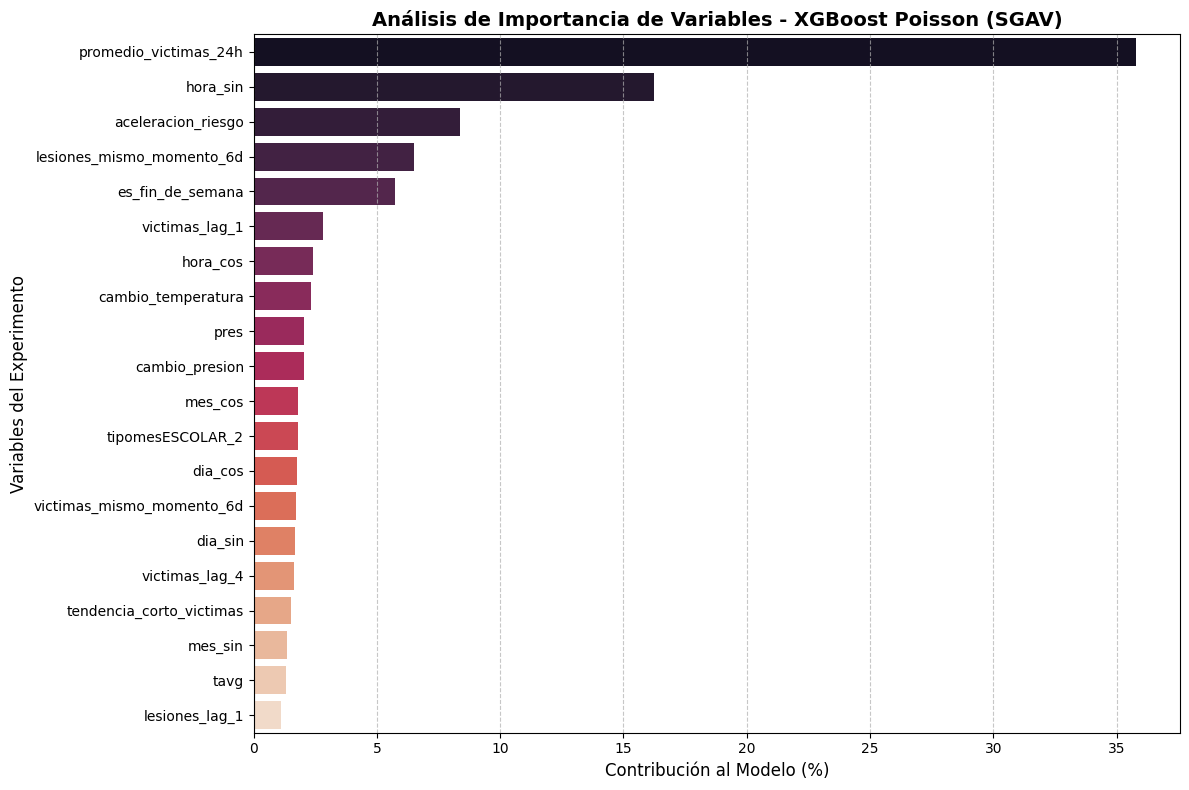
\includegraphics[width=\linewidth]{imagenes/image12.png}
\caption{Contribución de cada variable a la capacidad de predicción del modelo}
\label{fig:contribucion-de-cada-variable-a-la-capac}
\notaflot{\fuentepropia{}, según la salida del modelo entrenado.}
\end{figure}

Los resultados indican que la cantidad de víctimas en promedio en las últimas 24 tiene la mayor contribución a la predicción en orden del \qty{35}{\percent} aproximadamente, le sigue la componente función seno del bloque horario con \qty{15}{\percent} lo que deja entrever que el pasado cercano y el bloque horario en el cual se va a realizar la predicción contribuye a poco más del \qty{50}{\percent} a la predicción del modelo. Se podría afirmar entonces que el riesgo de que existan accidentes depende mayoritariamente de qué pasó en un pasado cercano en términos de cómo vienen evolucionando las víctimas como lo confirma el hecho de que de las primeras 6 variables concentran el \qty{80}{\percent} de la contribución a la predicción, 4 son variables referidas a que pasó y solo 2 están referidas al presente como lo es el caso de la franja horaria (\var{hora\_sin}) y si es fin de semana o no (\var{es\_fin\_de\_semana}).

También se puede observar que otras variables que se pensaban que podían influir notablemente como las climatológicas (\var{cambio\_temperatura}, pres, \var{cambio\_presion}, tavg) no son tan importantes para el modelo en cuestión en términos de aporte a la capacidad de predicción. Obtener esta información es de especial importancia a la hora de desarrollar el producto final, dado que si una variable resulta irrelevante o de baja utilidad puede optarse por no incluirla y en consecuencia no tener que recolectar, procesar, y entregar ese dato al modelo.

\begin{longtable}[]{@{}
>{\raggedright\arraybackslash}p{(\linewidth - 6\tabcolsep) * \real{0.2500}}
  >{\centering\arraybackslash}p{(\linewidth - 6\tabcolsep) * \real{0.2500}}
  >{\centering\arraybackslash}p{(\linewidth - 6\tabcolsep) * \real{0.2500}}
  >{\raggedright\arraybackslash}p{(\linewidth - 6\tabcolsep) * \real{0.2500}}@{}}
\caption{Métricas del modelo para la clase crítica (1) y métricas globales}
\label{tab:metricas-del-modelo-de-clasificacion-par}\\
\toprule\noalign{}
\textbf{Métrica} & \textbf{Porcentaje} & \textbf{Valor Decimal} & \textbf{Interpretación en el Sistema} \\
\midrule\noalign{}
\endfirsthead
\toprule\noalign{}
\textbf{Métrica} & \textbf{Porcentaje} & \textbf{Valor Decimal} & \textbf{Interpretación en el Sistema} \\
\midrule\noalign{}
\endhead
\bottomrule\noalign{}
\endlastfoot
Accuracy Global (Exactitud) & \qty{73.0}{\percent} & 0,73 & Porcentaje global de predicciones correctas sobre el total de casos. \\
Recall (Sensibilidad) en Crítico & \qty{87.4}{\percent} & 0,87 & Porcentaje de eventos críticos capturados. \\
Precisión en Crítico & \qty{77.8}{\percent} & 0,78 & Porcentaje de alertas emitidas que resultaron ser eventos críticos. \\
F1-Score en Crítico & \qty{82.3}{\percent} & 0,82 & Media armónica entre la Precisión y el Recall para la clase crítica. \\
\end{longtable}

\notaflot{Las métricas evalúan el desempeño focalizado en la detección oportuna de eventos de riesgo.}

En la \cref{tab:matriz-de-confusion-del-modelo-de-clasif} se presentaron los resultados agrupados en la matriz de confusión para los 557 datos de testeo; a partir de ellos se calculan las métricas de la \cref{tab:metricas-del-modelo-de-clasificacion-par}.

La exactitud (Accuracy Global) representa el porcentaje de las predicciones correctas (408) sobre los 557 casos de testeo, \qty{73}{\percent} se puede considerar como un buen resultado, pero no hay que perder de vista que representa ese porcentaje respecto de la distribución de la variable objetivo. Como se está intentando predecir un evento crítico como lo es un accidente vial, para los usuarios del producto interesa evaluar la performance específica para ello.

La sensibilidad (Recall) representa en este caso el porcentaje de eventos críticos reales que capturó el modelo, \qty{87.4}{\percent} también se considera un resultado bueno a priori (346 casos de 396). Para complementar esta métrica, se tiene además la precisión, que representa el porcentaje de alertas emitidas por el sistema que efectivamente resultaron ser accidentes en la realidad. Aquí se tiene un punto de especial relevancia dado que la precisión es percibida directamente por el usuario cuando usa el sistema, es decir, que de sí de 445 alarmas 346 son los accidentes reales ese porcentaje también afectará a cómo éste percibe el riesgo cuando ve una alerta. Si el modelo detectara el \qty{100}{\percent} de los accidentes (máximo Recall) emitiendo constantemente alertas entonces esto disminuye la precisión, provocando que el usuario se fatigue y baje la guardia al estar siempre alertado.

El F1-Score es una métrica ampliamente utilizada para evaluar el desempeño de modelos de clasificación, especialmente cuando existe un desbalance entre las clases o cuando resulta igualmente importante minimizar tanto los falsos positivos como los falsos negativos. Esta métrica corresponde a la media armónica entre la Precisión y la Sensibilidad (Recall), por lo que solo alcanza valores elevados cuando ambas presentan un buen desempeño de manera simultánea. A diferencia de la exactitud (Accuracy), el F1-Score ofrece una evaluación más representativa de la capacidad del modelo para identificar correctamente los casos pertenecientes a la clase de interés. En este caso, el F1-Score para la clase \enquote{Crítico} (al menos 1 accidente) alcanzó un valor de \qty{82.3}{\percent}.

\begin{longtable}[]{@{}
>{\raggedright\arraybackslash}p{(\linewidth - 4\tabcolsep) * \real{0.3333}}
  >{\centering\arraybackslash}p{(\linewidth - 4\tabcolsep) * \real{0.3333}}
  >{\raggedright\arraybackslash}p{(\linewidth - 4\tabcolsep) * \real{0.3333}}@{}}
\caption{Desempeño y errores del modelo en la clase normal (0)}
\label{tab:desempeno-y-errores-del-modelo-en-la-cla}\\
\toprule\noalign{}
\textbf{Métrica / Concepto} & \textbf{Valor} & \textbf{Interpretación en el Sistema} \\
\midrule\noalign{}
\endfirsthead
\toprule\noalign{}
\textbf{Métrica / Concepto} & \textbf{Valor} & \textbf{Interpretación en el Sistema} \\
\midrule\noalign{}
\endhead
\bottomrule\noalign{}
\endlastfoot
Recall (Sensibilidad) en Normal & \qty{39.0}{\percent} & Proporción de momentos seguros reales identificados. \\
Falsas Alertas (Falsos Positivos) & 99 & Situaciones sin incidentes en las que el sistema emitió erróneamente una alerta. \\
Críticos No Detectados (Falsos Negativos) & 50 & Situaciones con víctimas reales en las que el sistema omitió activar la alerta. \\
\end{longtable}

En este punto es donde se puede notar la dificultad fundamental de trabajar con predicciones de eventos como los accidentes viales. Cuando se analiza el desempeño para la clase normal (momentos seguros donde no hay accidentes) se tiene una sensibilidad de \qty{39}{\percent} producto de que se identifican correctamente 62 de 161 momentos seguros. Además se tiene 99 falsos positivos y 50 momentos en los cuales no se emite alerta a pesar de que hay víctimas. Estos resultados sugieren que el sistema no puede discriminar con gran capacidad momentos seguros y momentos riesgosos.

El XGBoost que se acaba de describir no es un modelo que pueda ser llevado a producción tal y como está, esto no quiere decir que no sirva, por el contrario, los modelos de línea de base son fundamentales para el desarrollo de productos basados en inteligencia artificial. Este en particular sirvió para generar una referencia para comparar los demas modelos que se entrenen, analizar cuales son las variables que más contribuyen a la capacidad predictiva, analizar qué métricas se deben observar y cuales no, selección de hiperparámetros, entre otros aspectos fundamentales como por ejemplo la forma en la que se agregan los datos que es fundamental no solo para el modelo propiamente dicho sino también a nivel requerimientos del producto final.

\section{Gestión del proyecto}\label{gestiuxf3n-del-proyecto}

\subsection{Definición de Requisitos}\label{definiciuxf3n-de-requisitos}

Para la definición de requisitos se tratan tanto aspectos generales para la gestión de un proyecto como lo pueden ser los objetivos y las partes interesadas como otros que son más específicos de proyectos de software como por ejemplo las restricciones en los datos, los modelos y su despliegue. En la siguiente sección se mencionan de forma resumida los principales requisitos que se relevaron y como se definieron, al final de la misma se podrá tener una idea de los objetivos, partes interesadas, restricciones de los datos y de los modelos, requisitos funcionales y no funcionales.

El objetivo de este proyecto es obtener un sistema que basado en el uso de inteligencia artificial permite tomar mejores decisiones a usuarios específicos del Ministerio Público Fiscal, en concreto los que trabajan en el área de accidentología vial. En este sentido también es válido aclarar para quien no es este producto, no es para personal de policía judicial, agentes de tránsito, personal municipal, ni ciudadanos en general. Teniendo esto en cuenta también se pueden definir las partes interesadas, a saber: Ministerio Público Fiscal, MPF Accidentología Vial, MPF Formación, LIDeSIA y FCEFyN.

Para poder alcanzar adecuadamente estos objetivos primero se deben establecer una serie de supuestos respecto de las restricciones que imponen los modelos para series temporales. Un algoritmo que predice el riesgo de accidentes viales generalmente necesita información en bloques discretos de tiempo, como por ejemplo en el caso de LightGBM y XGB, es decir que se requiere que los usuarios finales mantengan permanentemente actualizados los datos que son inputs para el modelo. En este proyecto, los bloques de predicción son de 6 horas y por lo tanto necesitamos poder agregar todos los datos conocidos en ese intervalo para poder realizar la predicción. Existen otros modelos que son más flexibles con este requerimiento, pero aquí hay que tener en cuenta otra restricción fundamental. Siendo que se está desarrollando el producto de forma tal que esté alineado con las normas ISO 42001 es necesario seleccionar un modelo que sea explicable (XAI). Se tiene entonces que asumir esta restricción y dar por supuesto que el equipo del MPF se compromete a mantener los datos actualizados.

En este punto es importante destacar que el alcance que se definió para la gestión de este proyecto es el acorde a un producto mínimo viable, es decir que si bien no se incluyen todas las características funcionales y no funcionales en el desarrollo (control de acceso basado en roles, cumplimiento de todos los puntos de las normas ISO 42001, Ciberseguridad, UX UI, etc), se trabaja teniendo en cuenta que en el futuro serán obligatorias y que por lo tanto se debe diseñar sin generar incompatibilidades.

En cuanto a la necesidad de realizar \eng{forecasting}, se justifica bajo la referencia B.6.2.2a (Requisitos y especificaciones del sistema de IA), surge como una evolución deseable del actual sistema de gestión descriptivo para pasar de la caracterización a la predicción. Estas especificaciones funcionales se traducen en un sistema de alerta temprana basado en la escala del puntaje estándar Z-score, el cual activa una alerta roja si el riesgo predicho supera las dos desviaciones estándar respecto al promedio, una alerta naranja si se ubica entre una y media y dos desviaciones, una alerta amarilla entre una y una y media desviaciones, y una alerta verde si la situación está controlada con un riesgo menor o igual a una desviación estándar.

\subsection{Dependencias tecnológicas y funcionales}\label{dependencias-tecnoluxf3gicas-y-funcionales}

Las dependencias tecnológicas y funcionales aplicables a un proyecto de software basado en inteligencia artificial pueden ser sumamente extensas dependiendo de la complejidad del sistema, dado que en este caso estamos analizando un MVP se tendrán en cuenta sólo las aplicables al alcance de una prueba de concepto de estas características.

Primeramente se deben analizar las dependencias funcionales, es decir, todas las condiciones del negocio o los procesos operativos en los cuales la intervención humana es necesaria para que el producto o sistema funcione. Se tiene por ejemplo el caso de la carga de datos, una falla en este proceso es vital para el sistema, si la información no se carga a tiempo o se introducen datos erróneos el resultado puede ser de impacto crítico en el caso de lo primero (el sistema queda inutilizable) o de impacto medio en el segundo caso (el sistema funciona pero con precisión reducida).

Por otra parte se tienen las dependencias tecnológicas, que son los componentes de hardware, software, servicios en la nube, APIs o bases de datos de los que depende la solución para recopilar datos, entrenar modelos o mostrar resultados. Con el mismo criterio mencionado anteriormente se destaca el Centro de Cómputos de Alto Desempeño, tanto en su servidor donde se aloja el servicio web como sus clusters de cómputo como Serafin o Mendieta donde se entrenan los modelos. El servidor de CCAD donde se aloja el servicio genera una dependencia crítica porque sin él es imposible alertar a los usuarios del MPF, en cambio, los clusters donde se entrenan los modelos no generan un impacto que comprometa al sistema dado que no es necesario reentrenar constantemente para mantener la precisión. Por último se encuentra una dependencia referida al consumo de APIs meteorológicas para la extracción de datos climáticos necesarios para realizar las predicciones, si bien es posible configurar el sistema para que tenga APIs como segunda opción (si la principal se cae), el impacto es bajo ya que no tener esta información disponible no reduce de manera significativa el desempeño del modelo.

\begin{longtable}[]{@{}
>{\raggedright\arraybackslash}p{(\linewidth - 4\tabcolsep) * \real{0.2281}}
  >{\raggedright\arraybackslash}p{(\linewidth - 4\tabcolsep) * \real{0.1927}}
  >{\raggedright\arraybackslash}p{(\linewidth - 4\tabcolsep) * \real{0.5428}}@{}}
\caption{Matriz de dependencias}
\label{tab:matriz-de-dependencias}\\
\toprule\noalign{}
\textbf{Dependencia} & \textbf{Tipo} & \textbf{Impacto} \\
\midrule\noalign{}
\endfirsthead
\toprule\noalign{}
\textbf{Dependencia} & \textbf{Tipo} & \textbf{Impacto} \\
\midrule\noalign{}
\endhead
\bottomrule\noalign{}
\endlastfoot
Carga de Datos & Funcional & Crítica: Se pierde la secuencialidad del modelo \\
Clasificacion Lesión & Funcional & Media: El modelo pierde precisión \\
CCAD Servidor & Tecnológica & Critica: El modelo no está disponible \\
CCAD Serafin & Tecnológica & Baja: Impide el reentrenamiento del modelo \\
API Meteo & Tecnológica & Media: El modelo pierde precisión \\
\end{longtable}

\notaflot{\fuentepropia{}.}

\subsection{Gestión de riesgos}\label{gestiuxf3n-de-riesgos}

La gestión de riesgos del sistema de Alerta Temprana de Accidentes Viales se estructuró siguiendo los lineamientos de la cláusula 6,1 de la norma ISO/IEC 42001:2023 a nivel general y por otro lado a la orientación metodológica de la norma ISO/IEC 23894:2023. La primera establece qué debe producir el proceso en términos de criterios definidos, una evaluación con resultados comparables, un plan de tratamiento y una evaluación de impacto. Mientras que la segunda aporta el procedimiento y, en particular, el relevamiento de fuentes de riesgo de su Anexo B, empleado en este documento como marco de identificación.

Es necesario distinguir dos ejercicios que la norma 42001 requiere por separado y que con frecuencia se confunden. La cláusula 6.1.2 refiere a la evaluación de los riesgos que afectan a los objetivos de la organización, mientras que la cláusula 6.1.4 refiere a la evaluación del impacto del sistema sobre individuos, grupos y sociedad. El presente apartado desarrolla el primero; el segundo se trata en el apartado siguiente. La relación entre ambos es de alimentación: los impactos identificados sobre terceros se incorporan al registro de riesgos en la medida en que generan exposición institucional, legal o reputacional para los organismos involucrados.

El alcance de esta evaluación comprende el ciclo completo del dato y de la predicción bajo el esquema de trabajo que se definió previamente a lo largo de este documento, que es de responsabilidad compartida: el Ministerio Público Fiscal es el origen de los datos y el destinatario de las alertas, mientras que el Laboratorio de Investigación y Desarrollo de Software e Inteligencia Artificial concentra el procesamiento, el entrenamiento y la generación de las predicciones. Al no delegar completamente la operación del sistema en su conjunto, se generan dos superficies de riesgo propias y se tratan como tales, el ingreso de datos y la emisión de alertas.

\subsection{Criterios de Riesgo}\label{criterios-de-riesgo}

Con el fin de que la evaluación produzca resultados comparables entre sí, se definieron escalas cualitativas de cuatro niveles para la probabilidad de ocurrencia y para la severidad del impacto. Se optó por cuatro niveles en lugar de los tres habituales para mantener coherencia con la codificación de cuatro colores adoptada por la capa de decisión del propio sistema. El nivel de riesgo resultante se obtiene del producto de ambos valores.

\begin{longtable}[]{@{}
>{\raggedright\arraybackslash}p{(\linewidth - 4\tabcolsep) * \real{0.1606}}
  >{\centering\arraybackslash}p{(\linewidth - 4\tabcolsep) * \real{0.0964}}
  >{\raggedright\arraybackslash}p{(\linewidth - 4\tabcolsep) * \real{0.7066}}@{}}
\caption{Escala de probabilidad de ocurrencia}
\label{tab:escala-de-probabilidad-de-ocurrencia}\\
\toprule\noalign{}
\textbf{Nivel} & \textbf{Valor} & \textbf{Criterio de asignación} \\
\midrule\noalign{}
\endfirsthead
\toprule\noalign{}
\textbf{Nivel} & \textbf{Valor} & \textbf{Criterio de asignación} \\
\midrule\noalign{}
\endhead
\bottomrule\noalign{}
\endlastfoot
Baja & 1 & No se ha observado durante el desarrollo y no existen indicios de que pueda materializarse en el horizonte del prototipo. \\
Media & 2 & Es plausible; existen condiciones que podrían habilitarla, aunque no se ha manifestado. \\
Alta & 3 & Se ha manifestado de forma ocasional durante el desarrollo o es esperable en condiciones normales de operación. \\
Muy alta & 4 & Se verifica de manera sistemática en la situación actual del proyecto. \\
\end{longtable}

\notaflot{\fuentepropia{} sobre la base de ISO/IEC 23894:2023.}

\begin{longtable}[]{@{}
>{\raggedright\arraybackslash}p{(\linewidth - 4\tabcolsep) * \real{0.1606}}
  >{\centering\arraybackslash}p{(\linewidth - 4\tabcolsep) * \real{0.0964}}
  >{\raggedright\arraybackslash}p{(\linewidth - 4\tabcolsep) * \real{0.7066}}@{}}
\caption{Escala de severidad del impacto}
\label{tab:escala-de-severidad-del-impacto}\\
\toprule\noalign{}
\textbf{Nivel} & \textbf{Valor} & \textbf{Criterio de asignación} \\
\midrule\noalign{}
\endfirsthead
\toprule\noalign{}
\textbf{Nivel} & \textbf{Valor} & \textbf{Criterio de asignación} \\
\midrule\noalign{}
\endhead
\bottomrule\noalign{}
\endlastfoot
Menor & 1 & Afecta la comodidad del desarrollo sin comprometer resultados ni usuarios. \\
Moderado & 2 & Degrada el desempeño del sistema o retrasa el cronograma, sin invalidar los resultados obtenidos. \\
Mayor & 3 & Invalida resultados, inutiliza temporalmente el sistema o afecta la confianza del usuario final en la herramienta. \\
Crítico & 4 & Compromete derechos de terceros, obligaciones legales del organismo o la viabilidad del proyecto. \\
\end{longtable}

\notaflot{\fuentepropia{} sobre la base de ISO/IEC 23894:2023.}

\begin{longtable}[]{@{}
>{\raggedright\arraybackslash}p{(\linewidth - 8\tabcolsep) * \real{0.1931}}
  >{\centering\arraybackslash}p{(\linewidth - 8\tabcolsep) * \real{0.1931}}
  >{\centering\arraybackslash}p{(\linewidth - 8\tabcolsep) * \real{0.1931}}
  >{\centering\arraybackslash}p{(\linewidth - 8\tabcolsep) * \real{0.1931}}
  >{\centering\arraybackslash}p{(\linewidth - 8\tabcolsep) * \real{0.1931}}@{}}
\caption{Matriz de nivel de riesgo}
\label{tab:matriz-de-nivel-de-riesgo}\\
\toprule\noalign{}
\textbf{Probabilidad / Impacto} & \textbf{Menor (1)} & \textbf{Moderado (2)} & \textbf{Mayor (3)} & \textbf{Crítico (4)} \\
\midrule\noalign{}
\endfirsthead
\toprule\noalign{}
\textbf{Probabilidad / Impacto} & \textbf{Menor (1)} & \textbf{Moderado (2)} & \textbf{Mayor (3)} & \textbf{Crítico (4)} \\
\midrule\noalign{}
\endhead
\bottomrule\noalign{}
\endlastfoot
Muy alta (4) & Amarillo (4) & Naranja (8) & Rojo (12) & Rojo (16) \\
Alta (3) & Verde (3) & Amarillo (6) & Naranja (9) & Rojo (12) \\
Media (2) & Verde (2) & Amarillo (4) & Amarillo (6) & Naranja (8) \\
Baja (1) & Verde (1) & Verde (2) & Verde (3) & Amarillo (4) \\
\end{longtable}

\notaflot{\fuentepropia{}. El valor entre paréntesis corresponde al producto de la probabilidad por el impacto.}

Respecto del nivel de riesgo declarado para la etapa actual se define en función del nivel de madurez tecnológica. Al tratarse de un prototipo en TRL 3 que no se encuentra desplegado en operación real y que no sustituye ningún procedimiento vigente del organismo, se aceptan sin acción los riesgos de nivel verde y amarillo. Los riesgos de nivel naranja se documentan con un tratamiento previsto que puede posponerse a etapas de mayor madurez. Los riesgos de nivel rojo requieren tratamiento explícito o, en su defecto, una declaración de aceptación fundamentada, y constituyen condición de salida hacia niveles TRL superiores.

\subsection{Identificación y Valoración de Riesgos}\label{identificaciuxf3n-y-valoraciuxf3n-de-riesgos}

La identificación se realizó recorriendo el catálogo de fuentes de riesgo del Anexo B de la norma ISO/IEC 23894:2023 y contrastando cada categoría contra las características concretas del sistema desarrollado. El relevamiento incorpora además las dependencias funcionales y tecnológicas documentadas en el apartado anterior, que constituyen la base de los riesgos R8 y R9. El resultado se presenta en la \cref{tab:registro-de-identificacion-y-valoracion-}.

\begin{longtable}[]{@{}
>{\raggedright\arraybackslash}p{(\linewidth - 10\tabcolsep) * \real{0.0698}}
  >{\raggedright\arraybackslash}p{(\linewidth - 10\tabcolsep) * \real{0.3813}}
  >{\raggedright\arraybackslash}p{(\linewidth - 10\tabcolsep) * \real{0.2524}}
  >{\centering\arraybackslash}p{(\linewidth - 10\tabcolsep) * \real{0.0483}}
  >{\centering\arraybackslash}p{(\linewidth - 10\tabcolsep) * \real{0.0483}}
  >{\centering\arraybackslash}p{(\linewidth - 10\tabcolsep) * \real{0.1665}}@{}}
\caption{Registro de identificación y valoración de riesgos}
\label{tab:registro-de-identificacion-y-valoracion-}\\
\toprule\noalign{}
\textbf{ID} & \textbf{Descripción del riesgo} & \textbf{Fuente de riesgo (Anexo B, ISO/IEC 23894)} & \textbf{P} & \textbf{I} & \textbf{Nivel} \\
\midrule\noalign{}
\endfirsthead
\toprule\noalign{}
\textbf{ID} & \textbf{Descripción del riesgo} & \textbf{Fuente de riesgo (Anexo B, ISO/IEC 23894)} & \textbf{P} & \textbf{I} & \textbf{Nivel} \\
\midrule\noalign{}
\endhead
\bottomrule\noalign{}
\endlastfoot
R1 & Errores de transcripción y falta de normalización derivados de la carga manual de los siniestros por parte del personal administrativo. & Calidad y procedencia de los datos & 3 & 3 & Naranja (9) \\
R2 & Latencia entre la ocurrencia del siniestro y su digitalización, que altera la posición temporal del evento en la serie. & Calidad de los datos / Complejidad del entorno & 4 & 3 & Rojo (12) \\
R3 & Sesgo de subregistro: la base contiene únicamente siniestros con intervención judicial y no representa la siniestralidad total de la ciudad. & Sesgo algorítmico & 4 & 2 & Naranja (8) \\
R4 & Reidentificación de personas involucradas por cruce de fecha, franja horaria, georreferenciación y tipo de lesión, no verificada hasta la fecha. & Privacidad y protección de datos & 3 & 4 & Rojo (12) \\
R5 & Fatiga de alerta por exceso de falsos positivos, con la consiguiente pérdida de confianza del usuario en la herramienta. & Nivel de automatización / Uso del sistema & 3 & 3 & Naranja (9) \\
R6 & Sesgo de automatización: delegación del juicio profesional en la salida del sistema sin contraste con otras fuentes. & Nivel de automatización & 2 & 3 & Amarillo (6) \\
R7 & Ausencia de un procedimiento formalizado de supervisión humana para validar o desestimar las alertas antes de su uso. & Supervisión humana / Uso del sistema & 3 & 3 & Naranja (9) \\
R8 & Indisponibilidad del servidor del CCAD que aloja el servicio, con interrupción total de la emisión de alertas. & Hardware e infraestructura & 2 & 3 & Amarillo (6) \\
R9 & Interrupción del suministro de datos climáticos por caída de la API meteorológica. & Complejidad del entorno de despliegue & 2 & 2 & Amarillo (4) \\
R10 & Uso desviado del sistema hacia finalidades no previstas, riesgo latente que se activaría con la incorporación de predicción georreferenciada por zonas. & Uso previsto / Impacto social & 2 & 3 & Amarillo (6) \\
R11 & Dependencia de personas clave y ausencia de un esquema definido de continuidad o transferencia del sistema. & Ciclo de vida del sistema de IA & 3 & 2 & Amarillo (6) \\
\end{longtable}

\notaflot{\fuentepropia{}. P: probabilidad; I: impacto, valorados según las \cref{tab:escala-de-probabilidad-de-ocurrencia,tab:escala-de-severidad-del-impacto}. El nivel resulta de la \cref{tab:matriz-de-nivel-de-riesgo}. Las categorías de fuente corresponden al Anexo B de ISO/IEC 23894:2023. Los riesgos R8 y R9 se corresponden con las dependencias de impacto crítico y medio identificadas en la matriz de dependencias tecnológicas y funcionales.}

\subsection{Plan de Mitigación de Riesgos}\label{plan-de-mitigacion-de-riesgos}

La \cref{tab:plan-de-mitigacion-de-riesgos} consigna el tratamiento propuesto para cada riesgo identificado y el nivel residual estimado al cierre de la etapa actual. Se indica asimismo el actor responsable, considerando el esquema de responsabilidad compartida mencionado al inicio del apartado.

\begin{longtable}[]{@{}
>{\raggedright\arraybackslash}p{(\linewidth - 6\tabcolsep) * \real{0.0697}}
  >{\raggedright\arraybackslash}p{(\linewidth - 6\tabcolsep) * \real{0.4770}}
  >{\raggedright\arraybackslash}p{(\linewidth - 6\tabcolsep) * \real{0.1768}}
  >{\raggedright\arraybackslash}p{(\linewidth - 6\tabcolsep) * \real{0.2412}}@{}}
\caption{Plan de mitigación de riesgos}
\label{tab:plan-de-mitigacion-de-riesgos}\\
\toprule\noalign{}
\textbf{ID} & \textbf{Tratamiento propuesto} & \textbf{Responsable} & \textbf{Residual en TRL 3} \\
\midrule\noalign{}
\endfirsthead
\toprule\noalign{}
\textbf{ID} & \textbf{Tratamiento propuesto} & \textbf{Responsable} & \textbf{Residual en TRL 3} \\
\midrule\noalign{}
\endhead
\bottomrule\noalign{}
\endlastfoot
R1 & Reducir. Validaciones automáticas de rango y consistencia en la etapa de curado, y documentación del diccionario de datos acordada con el equipo de datos del MPF. & LIDeSIA / Equipo de datos del MPF & Amarillo. Aceptado. \\
R2 & Reducir. Incorporación de la fecha de digitalización como variable de control, evaluación del desfase medio y definición de una ventana de corte que excluya los bloques aún incompletos. & LIDeSIA / MPF & Naranja. Condición de salida hacia TRL 4. \\
R3 & Aceptar con declaración. La población objetivo del sistema son precisamente los eventos con intervención judicial, por lo que el sesgo resulta parcialmente alineado con el caso de uso. Se documenta como limitación de generalización. & LIDeSIA & Naranja. Aceptado con declaración. \\
R4 & Reducir. Verificación de unicidad de los registros por combinación de cuasi-identificadores y, en caso de detectarse casos únicos, agregación espacial o temporal previa a cualquier publicación o difusión del conjunto de datos. & LIDeSIA / MPF & Rojo. Tratamiento pendiente y condición de salida hacia TRL 4. \\
R5 & Reducir. Calibración del umbral de decisión priorizando la precisión por sobre la sensibilidad, con aceptación explícita de la consecuencia que ello implica sobre los eventos no detectados, conforme a la política declarada en el apartado siguiente. & LIDeSIA & Amarillo. Tratamiento en curso. \\
R6 & Reducir. Comunicación de la alerta acompañada de su intervalo de predicción y no como valor puntual, y declaración del carácter complementario del sistema respecto del procedimiento vigente, de modo que la incertidumbre resulte visible para el usuario. & LIDeSIA & Amarillo. Aceptado. \\
R7 & Reducir, de forma compartida y diferida. Definición de un procedimiento de validación humana previa a la actuación, con registro de la decisión adoptada, prevista para la etapa de integración con el MPF. & MPF / LIDeSIA & Naranja. Condición de salida hacia TRL 4. \\
R8 & Aceptar con tratamiento diferido. Definición del requisito de disponibilidad y del esquema de contingencia prevista para la etapa de despliegue. & CCAD / LIDeSIA & Amarillo. Aceptado. \\
R9 & Evitar. Dado que el análisis de importancia de variables del modelo de línea de base evidenció una contribución marginal de las variables climáticas, se evalúa su exclusión del conjunto de entradas, lo que elimina la fuente de riesgo. Como alternativa, configuración de una fuente meteorológica secundaria. & LIDeSIA & Verde, sujeto a la confirmación de la exclusión de la variable. \\
R10 & Evitar. Declaración explícita del uso previsto y de los usos no admitidos del sistema, incorporada al apartado de definición de requisitos, y nueva evaluación de impacto como condición previa a la incorporación de predicción georreferenciada. & LIDeSIA / MPF & Amarillo. Latente. \\
R11 & Reducir. Documentación del código y de los procedimientos en repositorio versionado, como condición previa a cualquier esquema de transferencia. & LIDeSIA & Amarillo. Aceptado. \\
\end{longtable}

\notaflot{\fuentepropia{}. Las opciones de tratamiento corresponden a las categorías de ISO 31000:2018 adoptadas por ISO/IEC 23894:2023: evitar la fuente de riesgo, reducir la probabilidad o la consecuencia, compartir el riesgo con un tercero y aceptar el riesgo de forma informada. El nivel residual se estima al cierre de la etapa actual de madurez tecnológica.}

\subsection{Evaluación del Impacto del Sistema de IA}\label{evaluaciuxf3n-del-impacto-del-sistema-de-ia}

La cláusula 6.1.4 de la norma ISO/IEC 42001:2023, desarrollada en los apartados A.5 y B.5 de sus anexos, requiere evaluar las consecuencias del sistema sobre individuos, grupos y sociedad, con independencia del riesgo que el sistema representa para los objetivos de la organización.  La evaluación que sigue corresponde al estado actual del prototipo y debe repetirse en caso de haber cambios en el sistema o en su contexto de uso.

\subsection{Impacto Sobre Individuos y Grupos}\label{impacto-sobre-individuos-y-grupos}

El sistema no elabora perfiles individuales ni produce decisiones que afecten a personas en específico, es decir, la unidad de predicción es un bloque temporal de seis horas para el conjunto de toda la ciudad, y la salida es una estimación agregada de siniestralidad. En consecuencia, no se identifican decisiones automatizadas de efecto individual en el sentido de la normativa de protección de datos.

El impacto sobre individuos se concentra, por lo tanto, en el tratamiento de los datos de origen. La base fue anonimizada mediante la supresión de los nombres de las personas involucradas, conforme a lo previsto por la Ley N.º 25.326 de Protección de los Datos Personales. No obstante, la anonimización de identificadores directos no elimina por sí sola la posibilidad de reidentificación por cruce de cuasi-identificadores, y esta verificación no se realizó durante el desarrollo del prototipo. Se trata de una limitación reconocida, registrada como riesgo R4 y con tratamiento pendiente, que constituye condición previa a cualquier difusión del conjunto de datos fuera del ámbito de LIDeSIA.

Respecto al impacto sobre grupos, en su configuración actual el sistema opera sobre la totalidad de la ciudad de Córdoba sin segregación territorial, por lo que no produce salidas susceptibles de asociarse a un barrio, una zona o una población determinada.

\subsection{Conclusión de la Evaluación}\label{conclusiuxf3n-de-la-evaluaciuxf3n}

El nivel de riesgo residual del prototipo resulta aceptable para el nivel de madurez tecnológica TRL 3, en tanto el sistema todavía no se encuentra desplegado, no sustituye ningún procedimiento del organismo y sus salidas no alcanzan a individuos ni a grupos determinados. Esta aceptación no se extiende a niveles superiores, los riesgos R2 y R4 se establecen como condiciones de salida, es decir, deben encontrarse tratados con anterioridad a cualquier prueba en entorno operativo real.

\subsection{Flujograma de procesos}\label{flujograma-de-procesos}

\begin{figure}[htbp]
\centering

\includegraphics[width=\linewidth]{imagenes/image66.png}
\caption{Flujograma del proceso}
\label{fig:flujograma-del-proceso}
\notaflot{\fuentepropia{}.}
\end{figure}

Las secciones anteriores describieron por separado el tratamiento de los datos, la construcción del modelo y los mecanismos de gestión asociados. La \cref{fig:flujograma-del-proceso} los integra en una única representación de extremo a extremo, con el objeto de explicitar la secuencia completa que va desde el registro judicial del siniestro hasta la emisión de la alerta en la unidad judicial. Los elementos ubicados a la derecha de cada bloque indican el artefacto que produce esa etapa y que constituye la entrada de la siguiente, de modo que el flujo puede leerse tanto como secuencia de actividades como cadena de productos intermedios.

El proceso se inicia con la base cruda de siniestros, conformada por los registros que el personal administrativo de la Unidad Judicial de Accidentología Vial carga en el expediente al momento de la denuncia, según el procedimiento descripto en la sección 1.5. Sobre esa base se ejecuta la etapa de curación y anonimización, a cargo del equipo de datos del Ministerio Público Fiscal, que suprime la información sensible en cumplimiento de la Ley N.º 25.326 y entrega una base curada con el hecho como unidad de análisis. Esta es la única etapa del flujo en la que interviene información identificatoria, y por lo tanto la que concentra el tratamiento del riesgo R4.

La etapa siguiente transforma la base curada en el dataset consolidado, aplicando la agregación en bloques discretos de seis horas y la formulación autorregresiva supervisada detalladas en la sección 3.7.1. El producto de esta etapa es una serie temporal continua, en la que los bloques sin siniestros quedan representados por ceros, condición necesaria para que el modelo aprenda también las condiciones bajo las cuales no ocurren accidentes. Es en esta transición donde se materializa el riesgo R2, dado que un bloque cuyos siniestros aún no fueron digitalizados ingresa a la serie con un valor incompleto.

Sobre el dataset consolidado opera la etapa de entrenamiento y pronóstico, que produce el modelo de aprendizaje automático y su predicción para los bloques futuros. Su salida es un valor continuo que, por sí solo, no resulta interpretable para el usuario final. Por ese motivo el flujo incorpora una capa de decisión posterior, que traduce la salida numérica del modelo a una escala de niveles cromáticos según los umbrales definidos en la sección 3.8.1. Esta separación entre predicción y decisión es deliberada: permite recalibrar la sensibilidad del sistema sin reentrenar el modelo, y mantiene aislada la capacidad predictiva propia del algoritmo a los fines de su comparación con futuras versiones.

El flujo concluye con la emisión de la alerta a la unidad judicial, que constituye el punto de contacto entre el sistema y el usuario. Corresponde señalar que el diagrama representa el ciclo del dato y de la predicción, y no las acciones que el organismo adopta a partir de la alerta recibida. Ese componente, identificado en la sección 2.4.1 como capacidad de respuesta, excede el alcance del presente trabajo y queda pendiente para etapas de mayor madurez tecnológica.

Finalmente, el flujograma permite visualizar el esquema de responsabilidad compartida sobre el que se estructuró la gestión de riesgos. Las dos primeras etapas dependen del Ministerio Público Fiscal, las tres intermedias del Laboratorio de Investigación y Desarrollo de Software e Inteligencia Artificial, y la última vuelve a involucrar al organismo en calidad de destinatario. Las dos superficies de riesgo señaladas en la sección 3.8.3, el ingreso de datos y la emisión de alertas, se corresponden precisamente con los extremos de este flujo.

%% =====================================================================
%% 8. RESULTADOS
%% =====================================================================

\chapter{Resultados}\label{resultados}

Los resultados del presente trabajo deben ser abordados desde diferentes puntos de vista, por un lado tenemos los referidos al diseño del producto y las decisiones que se tomaron para ello, por otro lado los aspectos relacionados específicamente a inteligencia artificial y por último la gestión del producto como un todo.

El producto obtenido para el Ministerio Público Fiscal ya cuenta con las partes funcionales para ser desplegado posteriormente según como se definió inicialmente. Como se definió en los objetivos, se alcanzó un nivel de madurez tecnológica equivalente a TRL3, es decir que si bien el producto no fue probado en un entorno real operativo, se validaron todas sus partes y componentes fundamentales.

Respecto de los modelos utilizados para generar el \eng{forecasting} se puede resumir los resultados de la siguiente manera: Se tiene un modelo que consume todos los datos provistos por el MPF, la selección del mismo fue por múltiples criterios, como por ejemplo la velocidad de cómputo o la escalabilidad. Uno de los criterios más importantes para definirlo fue la explicabilidad del mismo, los árboles de decisión permiten comprender cómo es que el modelo está generando las predicciones. Respecto al rendimiento se alcanzó una performance adecuada para constituir una línea de base, es decir, permite obtener un nivel de exactitud útil y aceptable a partir del cual se podrá escalar mejorando los modelos y agregando nuevos datos. Además, el presente trabajo fue motivo de publicaciones, una para la Escuela de Perfeccionamiento en Investigación Operativa (2026), y otra para las jornadas de SINERGIA (2026), ambas en proceso de revisión a la fecha de elaboración de este documento.

A nivel gestión del producto y del proyecto se pueden destacar varias dimensiones que se fueron abordando a medida que este crecía. Se trabajó con un producto de punta a punta, es decir, comenzando por los requerimientos hasta obtener todas las partes de un sistema funcional. Para ello se investigó el qué y el por qué de cada proceso, de cada persona y de cada tecnología, para luego estudiar cómo la interacción de estos aspectos generan restricciones que deben ser superadas. El resultado final de este proceso es un producto que permite que un usuario no técnico disponga de funcionalidades impulsadas por inteligencia artificial que tendrán un impacto directo en la toma de decisiones en su día a día.

%% =====================================================================
%% 9. BIBLIOGRAFÍA
%% =====================================================================

% \nocite{*} incluye en el listado todas las fuentes de bibliografia.bib,
% no solo las citadas explícitamente en el texto (igual que en el
% documento original, que listaba todas las fuentes consultadas).
\nocite{*}
\printbibliography[title={Bibliografía},heading=bibintoc]

%% ---------------- Apéndices ----------------
\appendix

%% =====================================================================
%% 10. ANEXOS
%% =====================================================================

\chapter{Anexos}\label{anexos}

\section{Diccionario de datos de la base original}
\label{sec:diccionario-datos}

Este anexo documenta la estructura y el contenido del archivo fuente
\texttt{Siniestros unificados para nuevas variables julio 2025 v9 con distancias},
provisto por el equipo de datos del Ministerio Público Fiscal. Se reproducen los
nombres de campo tal como figuran en la planilla original, aun cuando su grafía no
sea homogénea, para preservar la trazabilidad con la fuente.

\subsection{Estructura de la planilla}
\label{ssec:estructura-planilla}

La base se organiza en tres niveles de análisis: el hecho siniestro, las personas
involucradas y la georreferenciación. Todas las hojas se vinculan por el número de
expediente (SAC), que opera como identificador único del siniestro.

\begin{table}[htbp]
\centering
\caption{Hojas que componen la planilla de cálculo original}
\label{tab:hojas-planilla}
\begin{tabular}{@{}>{\raggedright\arraybackslash}p{0.26\textwidth}
                  >{\raggedright\arraybackslash}p{0.52\textwidth}
                  >{\raggedleft\arraybackslash}p{0.12\textwidth}@{}}
\toprule
\textbf{Hoja} & \textbf{Contenido} & \textbf{Registros} \\
\midrule
\texttt{HECHO} & Siniestros con todas las variables del nivel hecho & 4906 \\
\texttt{Hecho solo georreferencia} & Subconjunto de siniestros efectivamente geocodificados & 4321 \\
\texttt{Códigos} & Catálogo de referencias de codificación de las hojas de hecho & --- \\
\texttt{Víctimas} & Datos simples de víctimas (sexo al nacer y edad simple) & 5673 \\
\texttt{Victagregada} & Víctimas agregadas por sexo al nacer y grupo etario & 4820 \\
\texttt{Denunciados} & Datos simples de denunciados (sexo al nacer y edad simple) & 5011 \\
\texttt{Denagregada} & Denunciados agregados por sexo al nacer y grupo etario & 4257 \\
\texttt{Personas} & Unión de víctimas y denunciados con una columna de rol & 10\,684 \\
\texttt{Georreferenciación} & Siniestros revisados en el proceso de geocodificación manual & 4884 \\
\bottomrule
\end{tabular}

\vspace{0.5em}
{\footnotesize \textit{Nota}. Elaboración propia sobre la planilla provista por el
Ministerio Público Fiscal. Cuando un mismo número de SAC correspondía a domicilios
distintos ---y por lo tanto a siniestros distintos--- se le añadió el sufijo
\texttt{.1} para desambiguarlo.}
\end{table}

\subsection{Variables de la hoja HECHO}
\label{ssec:variables-hecho}

\begin{longtable}{@{}>{\raggedright\arraybackslash}p{0.23\textwidth}
                    >{\raggedright\arraybackslash}p{0.44\textwidth}
                    >{\raggedright\arraybackslash}p{0.26\textwidth}@{}}
\caption{Diccionario de datos de la hoja HECHO}
\label{tab:diccionario-hecho} \\
\toprule
\textbf{Variable} & \textbf{Descripción} & \textbf{Valores o codificación} \\
\midrule
\endfirsthead

\multicolumn{3}{@{}l}{\footnotesize\textit{Tabla \ref{tab:diccionario-hecho} (continuación)}} \\
\toprule
\textbf{Variable} & \textbf{Descripción} & \textbf{Valores o codificación} \\
\midrule
\endhead

\midrule
\multicolumn{3}{r@{}}{\footnotesize\textit{Continúa en la página siguiente}} \\
\endfoot

\bottomrule
\endlastfoot

\multicolumn{3}{@{}l}{\textit{Identificación y variables temporales}} \\
\addlinespace
\texttt{Nro.\ de SAC} & Número de expediente; identificador único del siniestro & Alfanumérico \\
\texttt{Fecha de ingreso} & Fecha de ingreso del expediente, aproximada a la del siniestro & Fecha \\
\texttt{Hora del hecho} & Hora real del siniestro consignada en el expediente & Formato 24 h \\
\texttt{franja\_horaria} & Bloque horario de seis horas en que ocurre el siniestro & 1 = madrugada (0--6 h); 2 = mañana (6--12 h); 3 = tarde (12--18 h); 4 = noche (18--24 h) \\
\texttt{dia\_semana\_cat} & Día de la semana & 1 = lunes \ldots\ 7 = domingo \\
\texttt{es\_fin\_de\_semana} & Indica si el siniestro ocurre en fin de semana & 1 = sí; 2 = no \\
\texttt{es\_hora\_punta} & Indica si el siniestro ocurre en hora pico & 1 = sí (7:30--9:30, 12:00--14:00 y 17:30--19:30 h); 2 = no \\
\texttt{tipomesESCOLAR} & Régimen del mes según el calendario escolar y laboral & 1 = laboral/escolar (marzo a noviembre); 2 = no laboral (diciembre a febrero) \\
\texttt{estacionCLIMA} & Estación del año & 1 = otoño; 2 = invierno; 3 = primavera; 4 = verano \\
\addlinespace

\multicolumn{3}{@{}l}{\textit{Consecuencias del siniestro}} \\
\addlinespace
\texttt{Lesiones} & Tipo de lesiones según la carátula del expediente & Texto libre \\
\texttt{Lesionescod} & Codificación del tipo de lesiones & 1 = leves; 2 = graves; 3 = homicidio; 4 = otras \\
\addlinespace

\multicolumn{3}{@{}l}{\textit{Vehículos involucrados}} \\
\addlinespace
\texttt{Vehículo} & Vehículo 1 involucrado en el hecho & Texto libre \\
\texttt{VEHICULO1COD} & Codificación del vehículo 1 & Entero \\
\texttt{Vehiculo2} & Vehículo 2 o combinación de vehículos; los múltiples se separan con guion medio & Texto libre \\
\texttt{VEHICULO2COD} & Codificación del vehículo 2; se toma el más pesado del conjunto & Entero \\
\texttt{Transporte publico1} & Indica si el vehículo 1 es transporte público de pasajeros (colectivo, trolebús) & 1 = sí; 2 = no \\
\texttt{Transporte publico2} & Indica si el vehículo 2 es transporte público de pasajeros & 1 = sí; 2 = no \\
\texttt{Inmovil1} & Indica si el vehículo 1 es un objeto fijo (árbol, pared, reja, poste) & 1 = sí; 2 = no \\
\texttt{Inmovil2} & Indica si el vehículo 2 es un objeto fijo & 1 = sí; 2 = no \\
\texttt{Motorizado1} & Indica si el vehículo 1 es motorizado & 1 = sí; 2 = no \\
\texttt{Motorizado2} & Indica si el vehículo 2 es motorizado & 1 = sí; 2 = no \\
\texttt{Tamaño1} & Tamaño del vehículo 1 según su peso aproximado & Texto libre \\
\texttt{tam1cod} & Codificación del tamaño del vehículo 1 & 1 = persona; 2 = ligero; 3 = mediano; 4 = medio pesado; 5 = pesado \\
\texttt{Tamaño2} & Tamaño del vehículo 2 según su peso aproximado & Texto libre \\
\texttt{tam2cod} & Codificación del tamaño del vehículo 2 & 1 = persona; 2 = ligero; 3 = mediano; 4 = medio pesado; 5 = pesado \\
\texttt{TOTAL\_VEHICULOS} & Cantidad total de vehículos involucrados & Entero \\
\texttt{Complejidad} & Tipo de colisión según los actores involucrados & Texto libre \\
\texttt{Complejcod} & Codificación del tipo de colisión & 1 = casual o sin dato; 2 = dupla; 3 = múltiple \\
\texttt{involbici} & Indica si intervino al menos una bicicleta & 1 = sí; 2 = no \\
\texttt{involPeaton} & Indica si intervino al menos un peatón & 1 = sí; 2 = no \\
\addlinespace

\multicolumn{3}{@{}l}{\textit{Personas involucradas}} \\
\addlinespace
\texttt{V\_Fem} & Cantidad de víctimas de sexo femenino & Entero \\
\texttt{V\_Masc} & Cantidad de víctimas de sexo masculino & Entero \\
\texttt{V\_ninos} & Cantidad de víctimas del grupo etario niños & Entero \\
\texttt{V\_joven} & Cantidad de víctimas del grupo etario jóvenes & Entero \\
\texttt{V\_adulto} & Cantidad de víctimas del grupo etario adultos & Entero \\
\texttt{V\_adumayor} & Cantidad de víctimas del grupo etario adultos mayores & Entero \\
\texttt{D\_Fem} & Cantidad de denunciados de sexo femenino & Entero \\
\texttt{D\_Masc} & Cantidad de denunciados de sexo masculino & Entero \\
\texttt{D\_ninos} & Cantidad de denunciados del grupo etario niños & Entero \\
\texttt{D\_joven} & Cantidad de denunciados del grupo etario jóvenes & Entero \\
\texttt{D\_adulto} & Cantidad de denunciados del grupo etario adultos & Entero \\
\texttt{D\_adumayor} & Cantidad de denunciados del grupo etario adultos mayores & Entero \\
\texttt{victimas} & Cantidad total de víctimas del siniestro & Entero \\
\texttt{denunciados} & Cantidad total de denunciados del siniestro & Entero \\
\texttt{TotalPersonas} & Cantidad total de personas involucradas & Entero \\
\addlinespace

\multicolumn{3}{@{}l}{\textit{Localización y entorno vial}} \\
\addlinespace
\texttt{Latitud} & Latitud del punto de ocurrencia & Grados decimales \\
\texttt{Longitud} & Longitud del punto de ocurrencia & Grados decimales \\
\texttt{tipoVÍA} & Clasificación de la red vial según la ordenanza municipal 8060 & Texto libre \\
\texttt{TIPOVIA2} & Jerarquía de la vía, con bandas de 20 metros & Vía arterial-sectorial; vías de barrio \\
\texttt{Num Semáforo} & Identificador del semáforo más cercano & Alfanumérico \\
\texttt{Distancia Semáforo METROS} & Distancia radial al semáforo más cercano & Metros \\
\texttt{ConSemaforo} & Indica si hay un semáforo a 100 metros o menos & 1 = sí; 2 = no \\
\texttt{IDVERTICE} & Identificador del vértice (esquina) más cercano & Alfanumérico \\
\texttt{DIST VERTICE METROS} & Distancia radial a la esquina más cercana & Metros \\
\texttt{Enesquina} & Indica si el siniestro ocurrió a 15 metros o menos de un vértice & 1 = sí; 2 = no \\
\texttt{IDLUMINARIA} & Identificador de la luminaria más cercana & Alfanumérico \\
\texttt{DIST LUMINARIA METROS} & Distancia radial a la luminaria más cercana & Metros \\
\addlinespace

\multicolumn{3}{@{}l}{\textit{Condiciones solares y de luminosidad}} \\
\addlinespace
\texttt{amanece} & Hora de inicio del crepúsculo matutino & Formato 24 h \\
\texttt{salidasol} & Hora de salida del sol & Formato 24 h \\
\texttt{acimut1} & Acimut solar en la salida del sol, medido en sentido horario desde el norte geográfico & Grados (0--360) \\
\texttt{mediodía} & Hora en que el sol alcanza el cenit & Formato 24 h \\
\texttt{anochece} & Hora de inicio del crepúsculo vespertino & Formato 24 h \\
\texttt{acimut2} & Acimut solar en la puesta del sol, medido en sentido horario desde el norte geográfico & Grados (0--360) \\
\texttt{puesta} & Hora de puesta del sol & Formato 24 h \\
\texttt{horasxdia} & Duración total de la luz solar del día & Horas \\
\texttt{dianoche} & Indica si el siniestro ocurrió dentro o fuera del horario solar & Dentro del horario solar; fuera del horario solar \\
\texttt{LUMI\_NOCHE} & Disponibilidad de luminaria a 15 metros o menos en siniestros nocturnos & No había luminaria; es día, no usa luminaria; había luminaria \\
\end{longtable}

{\footnotesize \textit{Nota}. Elaboración propia sobre el documento de descripción de
datos provisto por el Ministerio Público Fiscal. Los nombres de campo se reproducen
con la grafía de la planilla original.}

\subsection{Notas metodológicas de la fuente}
\label{ssec:notas-fuente}

\paragraph{Georreferenciación.} La geocodificación se realizó de forma manual, caso por
caso, ubicando cada siniestro sobre cartografía en línea y registrando las coordenadas
de latitud y longitud. De los 4906 expedientes identificados como siniestros, 585 no
pudieron ubicarse con precisión ---mayoritariamente hechos sobre rutas referenciadas por
altura kilométrica o con descripciones ambiguas de la ubicación--- y 5 correspondían a
otra localidad. Quedaron así 4321 siniestros georreferenciados dentro del ejido de la
ciudad de Córdoba.

\paragraph{Clasificación de vehículos.} Se leyeron individualmente algo más de 9000
registros de expediente para identificar y clasificar los vehículos intervinientes
(automóvil, colectivo, motocicleta, utilitario, camión, entre otros). En ese proceso se
detectaron siniestros de tipo casual, con un único vehículo involucrado contra un objeto
inmóvil.

\paragraph{Grupos etarios.} La segmentación por edad sigue las recomendaciones de la
Organización Mundial de la Salud: niños (0 a 14 años), jóvenes (15 a 26 años), adultos
(27 a 59 años) y adultos mayores (60 años o más).

\paragraph{Variables solares.} Los horarios de salida y puesta del sol, crepúsculos,
acimut y duración del día se obtuvieron del \textit{Astronomical Applications Department}
del Observatorio Naval de los Estados Unidos, contrastados con los datos del Servicio de
Hidrografía Naval argentino. Se utilizó esa fuente por permitir la extracción tabular de
un año completo en una sola consulta, parametrizada para las coordenadas de la ciudad de
Córdoba.\footnote{\url{https://aa.usno.navy.mil/calculated/mrst}}

\paragraph{Revisión de variables.} En una instancia posterior de revisión se depuraron
las columnas de inmovilizados y las codificaciones redundantes; se unificó la
información de transporte público en una única variable de intervención, independiente
de la complejidad del hecho; y se redefinió la variable de complejidad como tipo de
colisión, con las categorías dupla (dos vehículos motorizados), múltiple (tres o más),
peatón contra vehículo motorizado, bicicleta contra vehículo motorizado, objeto contra
vehículo motorizado y otros. En la misma instancia se incorporaron las variables
\texttt{involbici} e \texttt{involPeaton}.

\section{Visualizaciones exploratorias complementarias}
\label{sec:visualizaciones-exploratorias}

Este anexo reúne el conjunto completo de visualizaciones generadas durante la etapa de
exploración de datos descripta en la \cref{exploraciuxf3n-de-datos}, sobre la base
consolidada de 4320 siniestros viales georreferenciados (julio de 2022 a junio de 2024).
Se incluyen aquí para no sobrecargar el cuerpo principal del informe, dado que solo una
selección de estas figuras se referencia directamente en el análisis.

\begin{figure}[htbp]
\centering
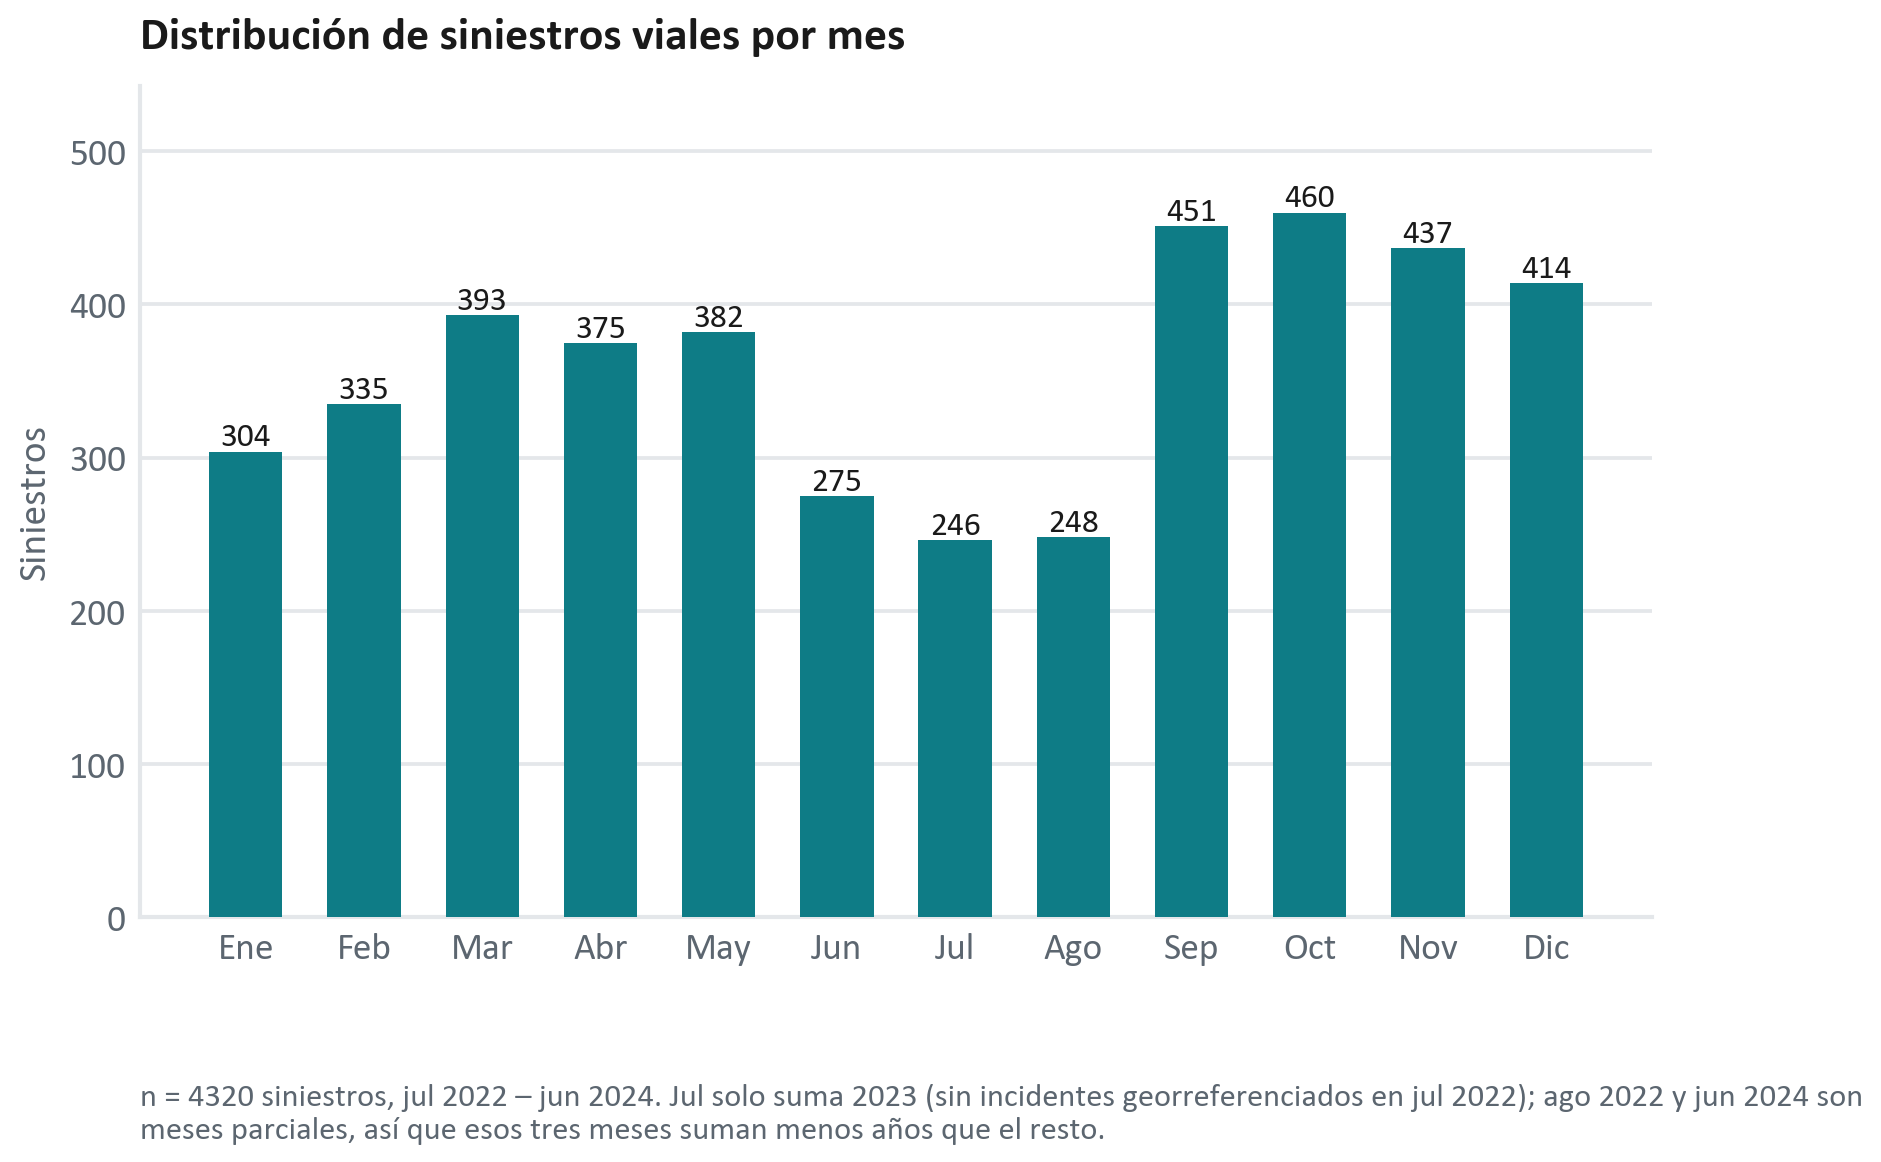
\includegraphics[width=0.85\linewidth]{imagenes/anexo_a2_distribucion_mes.png}
\caption{Distribución de siniestros viales por mes}
\label{fig:anexo-distribucion-mes}
\notaflot{Frecuencia mensual de siniestros georreferenciados (n = 4320), julio 2022 --
junio 2024. El máximo se registra en octubre (460) y el mínimo en julio (246); julio
computa únicamente 2023, y agosto de 2022 y junio de 2024 son meses parciales, por lo
que esos tres meses acumulan menos años que el resto. \fuentepropia{}.}
\end{figure}

\begin{figure}[htbp]
\centering
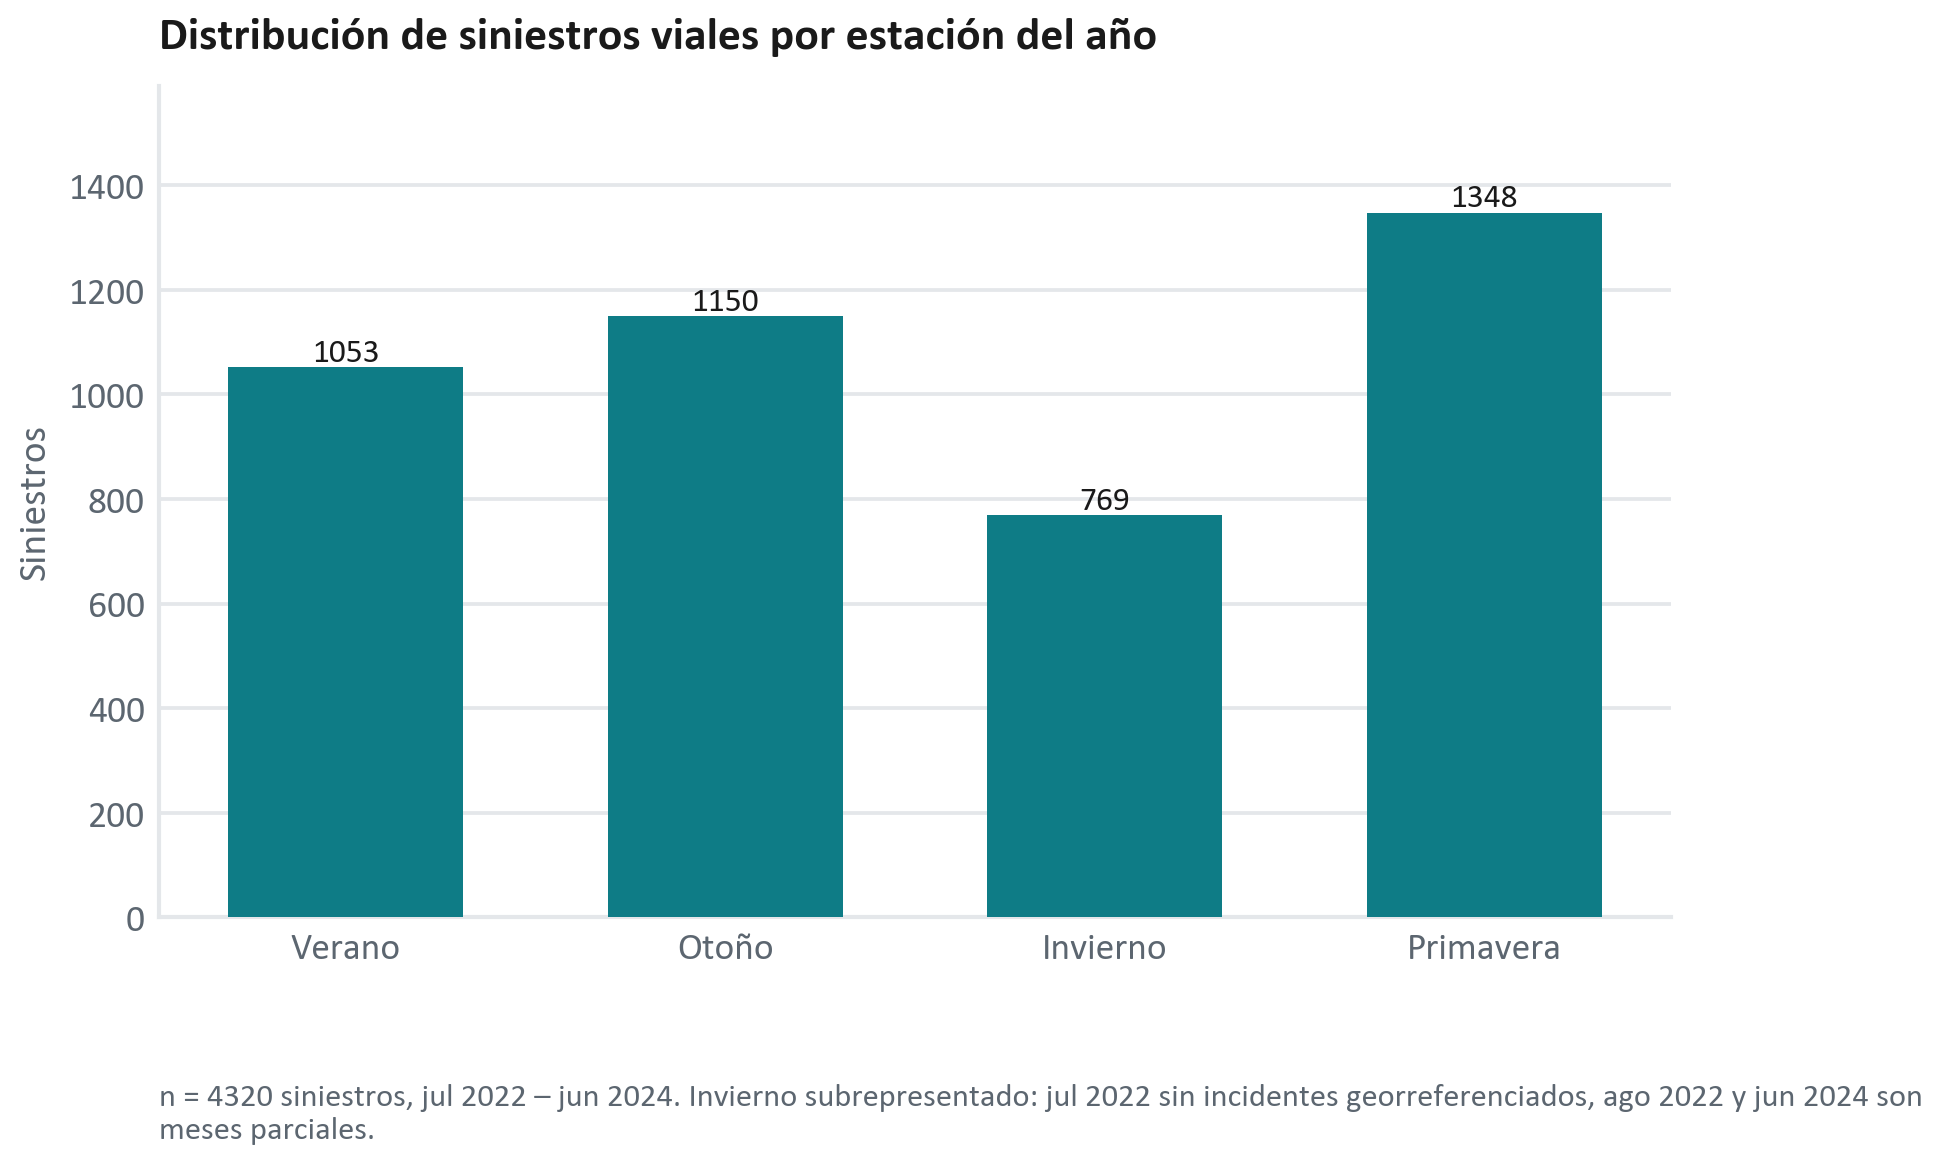
\includegraphics[width=0.8\linewidth]{imagenes/anexo_a2_distribucion_estacion.png}
\caption{Distribución de siniestros viales por estación del año}
\label{fig:anexo-distribucion-estacion}
\notaflot{Agregación estacional de los mismos 4320 siniestros. La primavera concentra
la mayor frecuencia (1348) y el invierno la menor (769), aunque esta última estación
está subrepresentada porque julio de 2022 no registra incidentes georreferenciados y
agosto de 2022 y junio de 2024 son meses parciales. \fuentepropia{}.}
\end{figure}

\begin{figure}[htbp]
\centering
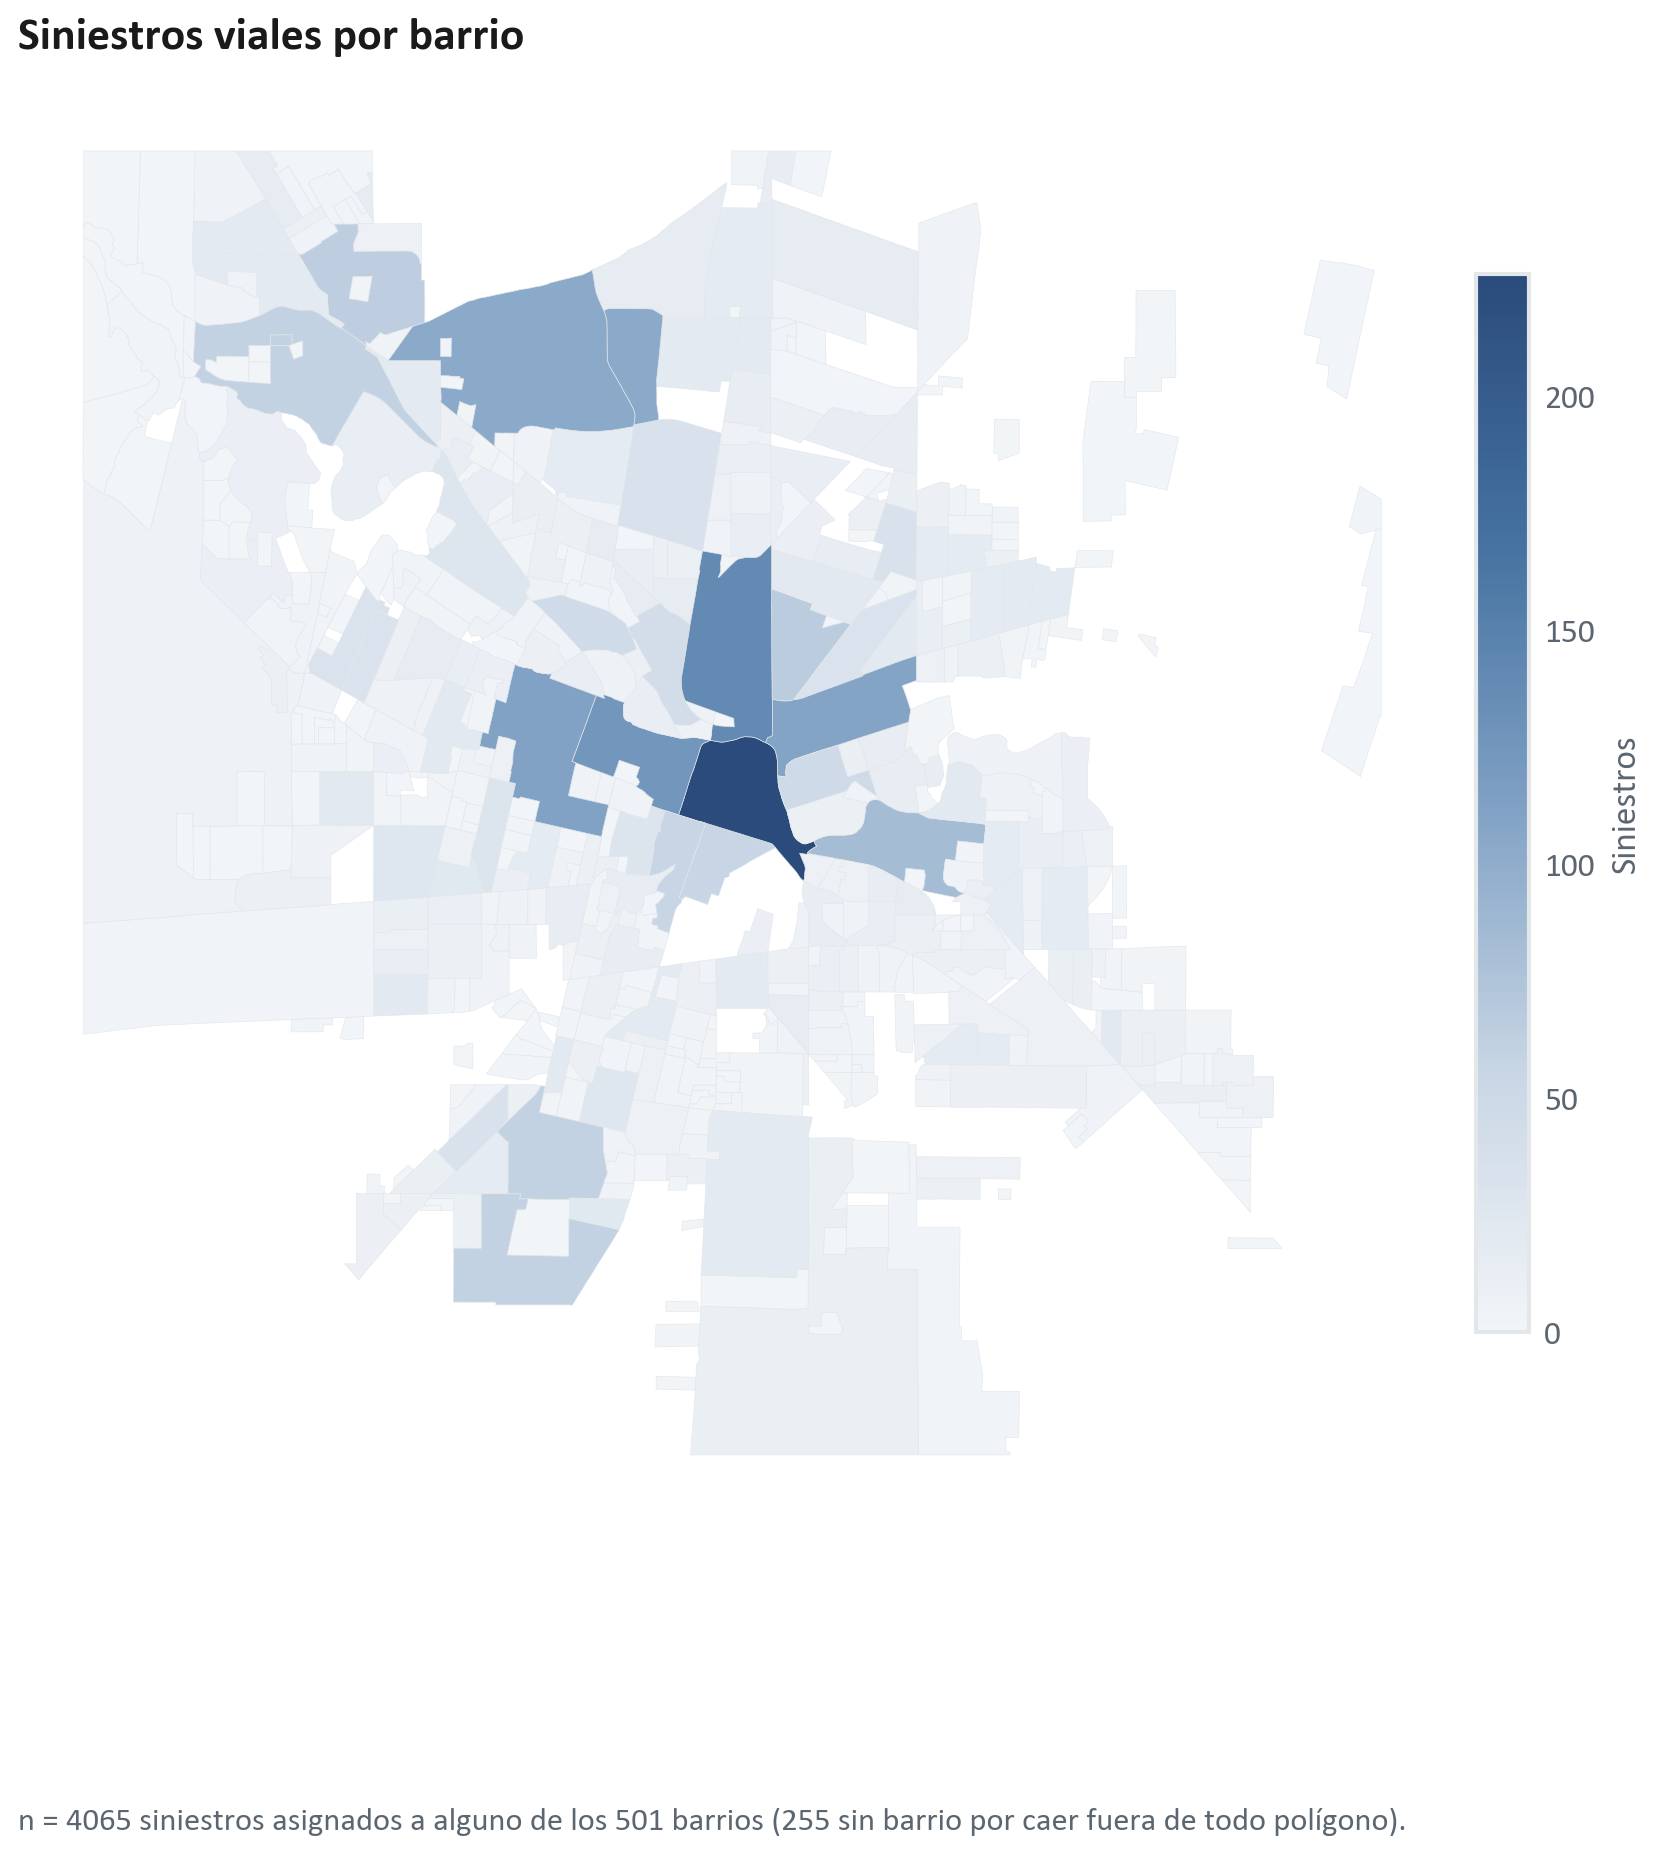
\includegraphics[width=0.62\linewidth]{imagenes/anexo_a2_mapa_calor_barrio.png}
\caption{Siniestros viales por barrio de la ciudad de Córdoba}
\label{fig:anexo-mapa-calor-barrio}
\notaflot{Cantidad de siniestros agregados por barrio (n = 4065 asignados a alguno de
los 501 polígonos vigentes; 255 casos cayeron fuera de todo polígono y quedaron sin
barrio asignado). El área central y sus barrios inmediatos concentran los valores más
altos, con un máximo superior a 200 siniestros en el polígono central. \fuentepropia{}.}
\end{figure}

\begin{figure}[htbp]
\centering
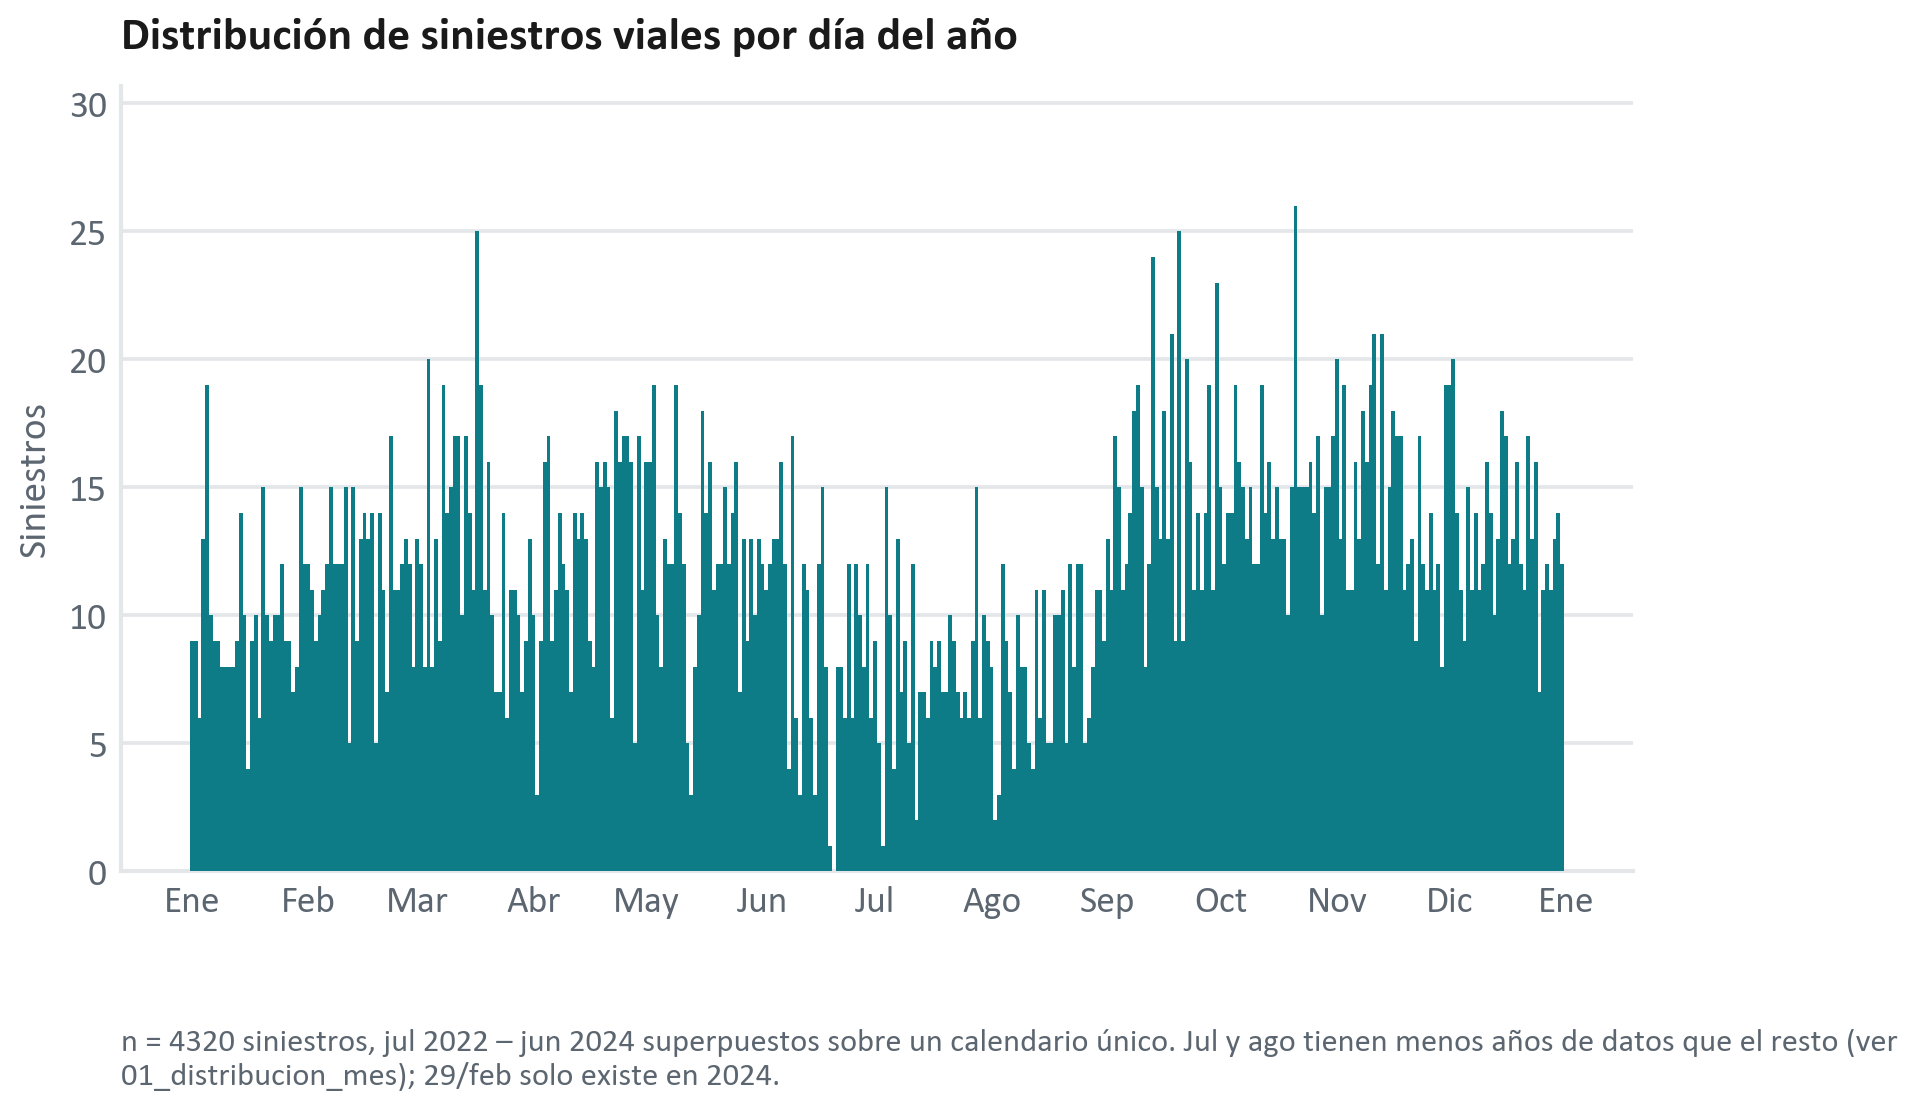
\includegraphics[width=0.85\linewidth]{imagenes/anexo_a2_distribucion_dia_anio.png}
\caption{Distribución de siniestros viales por día del año}
\label{fig:anexo-distribucion-dia-anio}
\notaflot{Frecuencia diaria de siniestros superpuesta sobre un calendario único de 365
días (n = 4320). Julio y agosto acumulan menos años de datos que el resto del
calendario, y el 29 de febrero solo existe en el año 2024, por lo que esos días deben
interpretarse con esa salvedad. Se observa mayor concentración entre septiembre y
noviembre. \fuentepropia{}.}
\end{figure}

\begin{figure}[htbp]
\centering
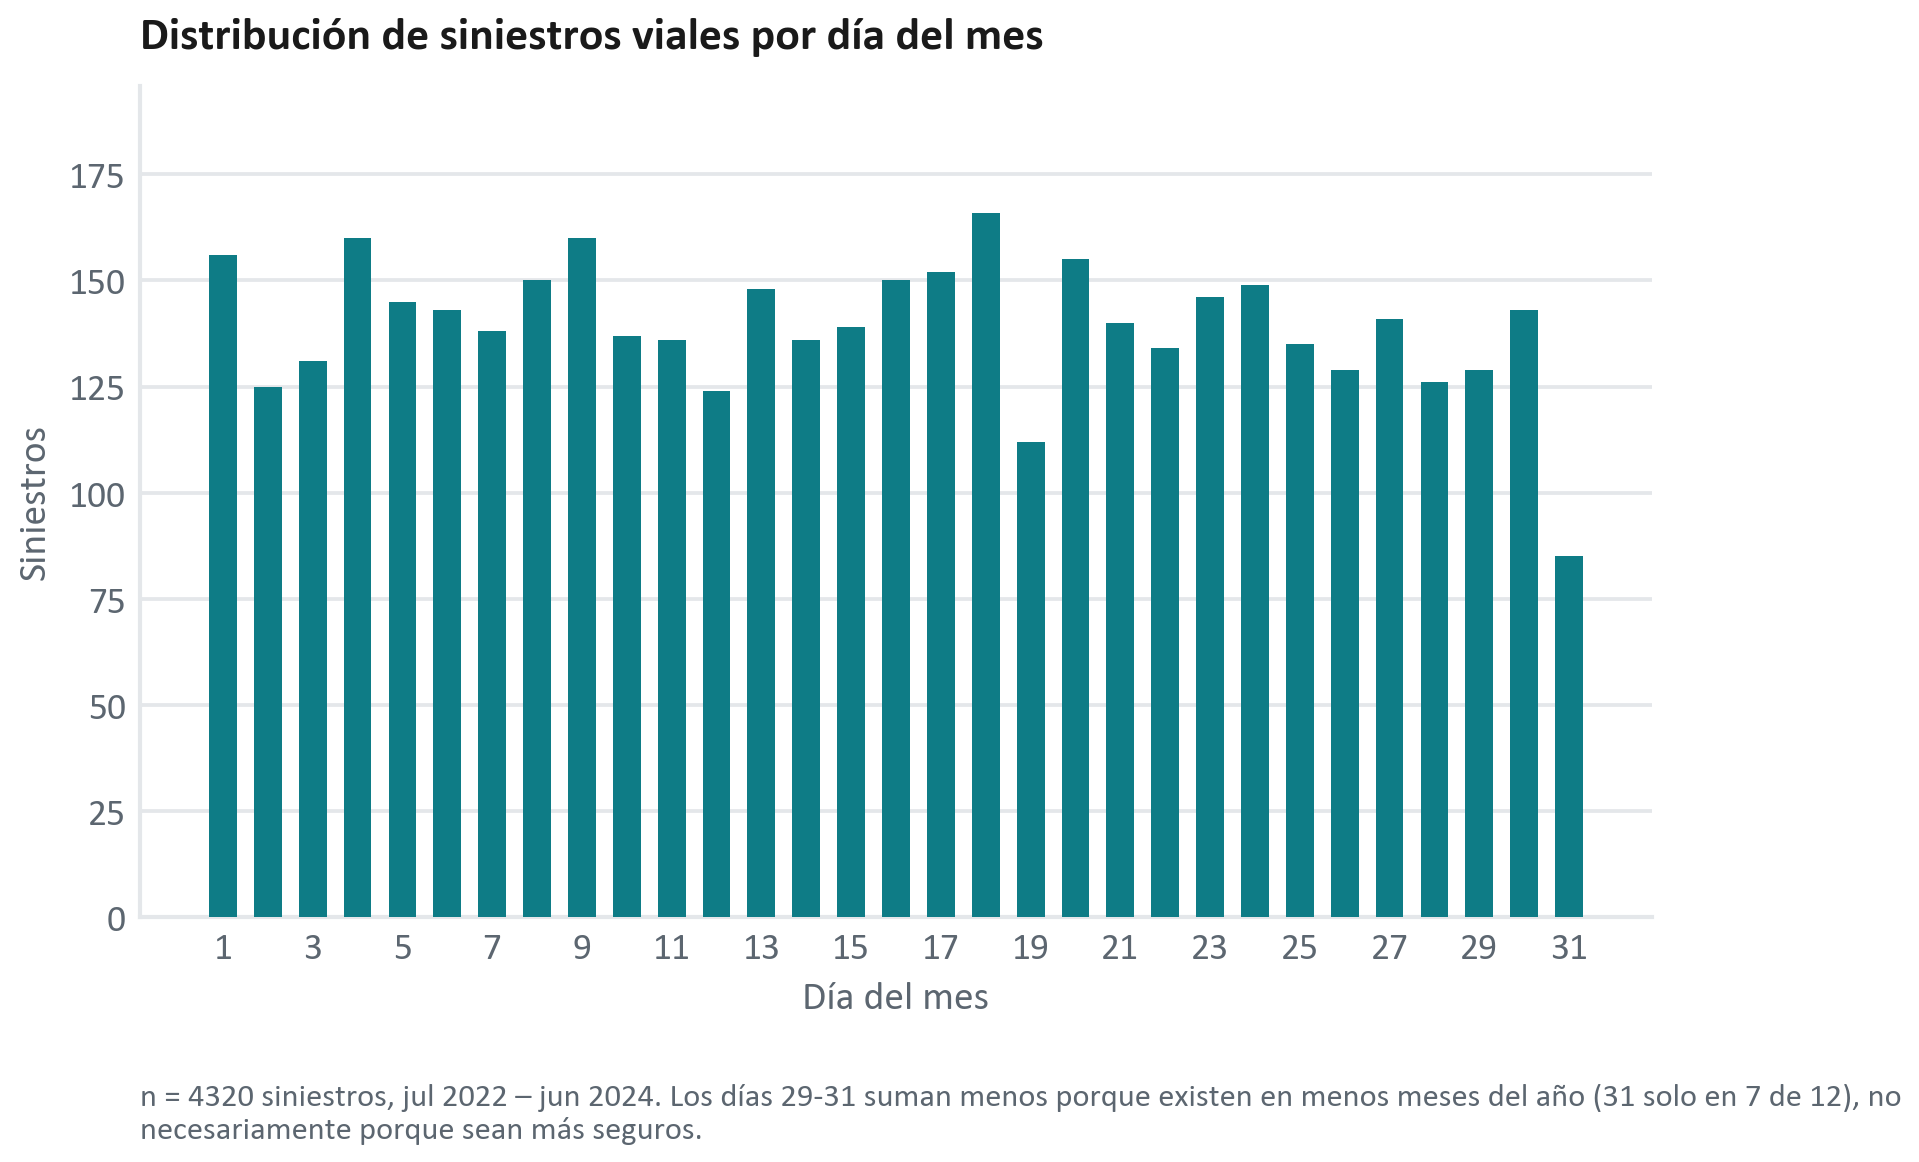
\includegraphics[width=0.85\linewidth]{imagenes/anexo_a2_distribucion_dia_mes.png}
\caption{Distribución de siniestros viales por día del mes}
\label{fig:anexo-distribucion-dia-mes}
\notaflot{Frecuencia de siniestros según el número de día calendario, sin distinguir
el mes (n = 4320). La distribución es relativamente uniforme entre los días 1 y 28; la
caída hacia el día 31 responde a que ese día solo existe en 7 de los 12 meses del año,
y no a un efecto real sobre la siniestralidad. \fuentepropia{}.}
\end{figure}

\begin{figure}[htbp]
\centering
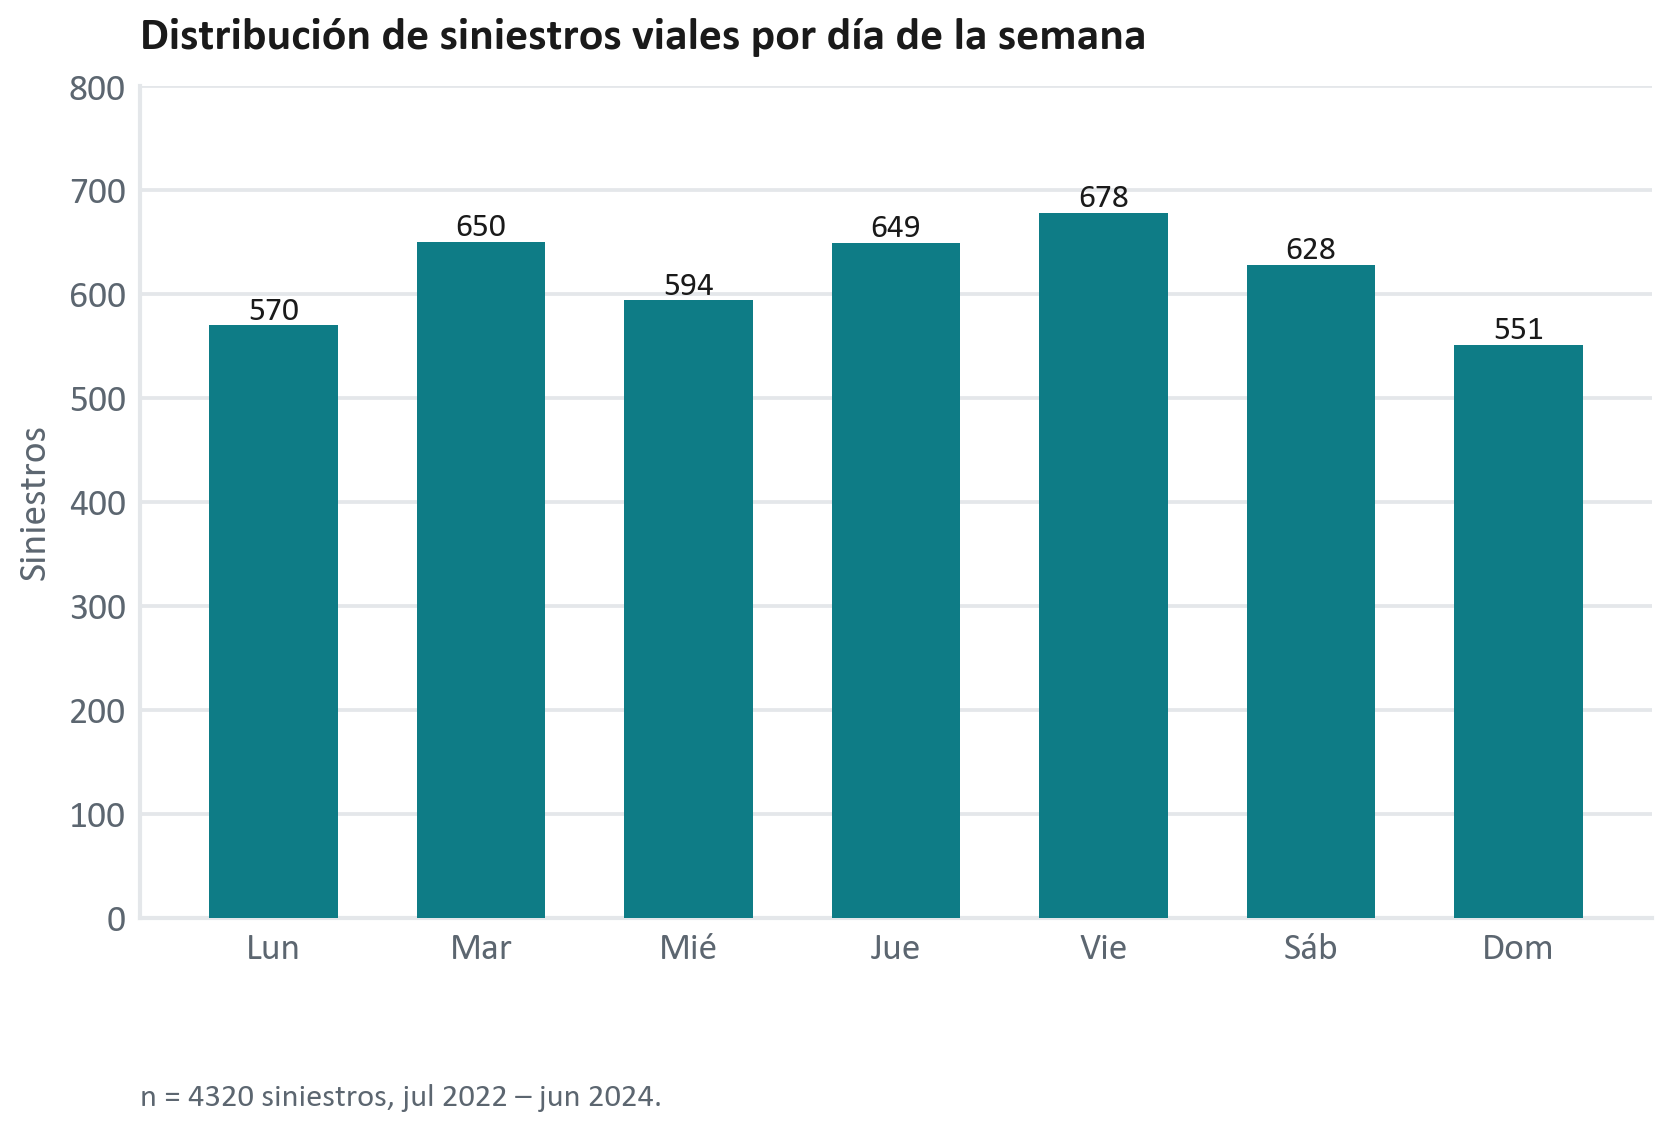
\includegraphics[width=0.85\linewidth]{imagenes/anexo_a2_distribucion_dia_semana.png}
\caption{Distribución de siniestros viales por día de la semana}
\label{fig:anexo-distribucion-dia-semana}
\notaflot{Frecuencia según día de la semana (n = 4320). El viernes concentra el máximo
(678) y el domingo el mínimo (551), con una distribución por lo demás relativamente
pareja entre martes y sábado. \fuentepropia{}.}
\end{figure}

\begin{figure}[htbp]
\centering
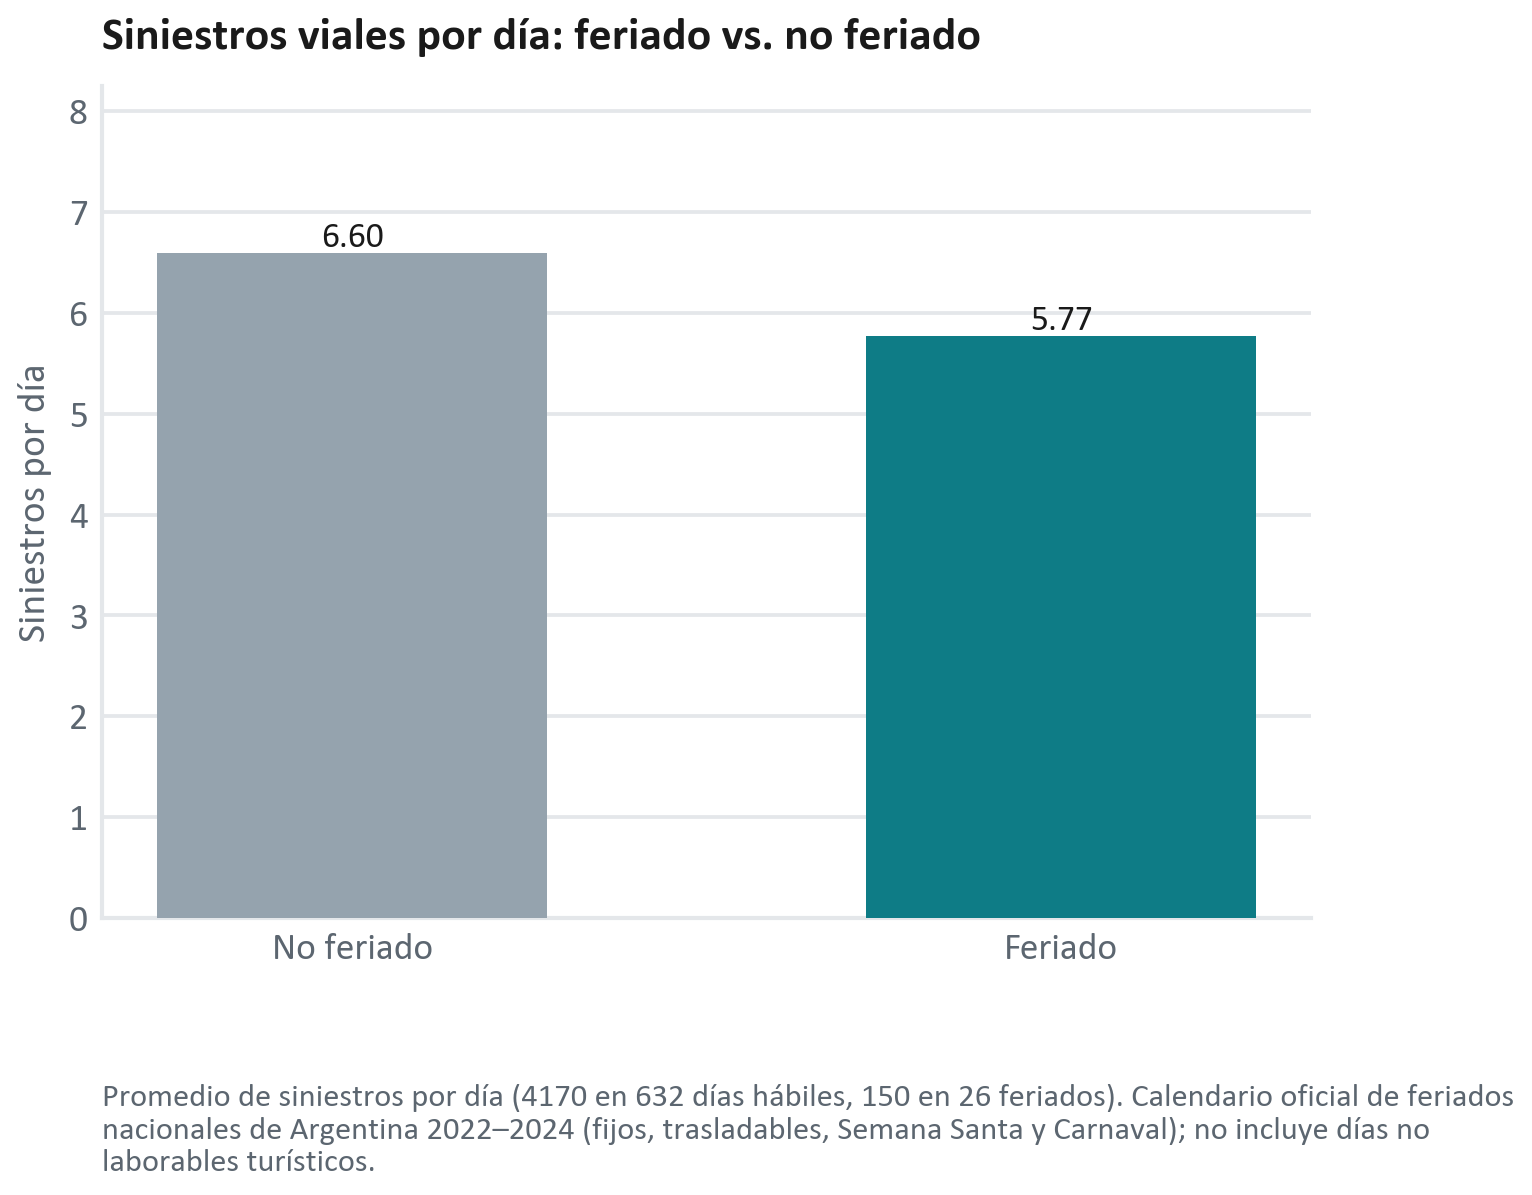
\includegraphics[width=0.75\linewidth]{imagenes/anexo_a2_feriado.png}
\caption{Siniestros viales por día: feriado frente a no feriado}
\label{fig:anexo-feriado}
\notaflot{Promedio de siniestros por día calendario, distinguiendo feriados
nacionales de días no feriados (4170 siniestros en 632 días hábiles y 150 en 26
feriados, según el calendario oficial de feriados de Argentina 2022--2024; no se
incluyen días no laborables turísticos). El promedio diario resulta levemente menor en
los feriados (5,77 frente a 6,60). \fuentepropia{}.}
\end{figure}

\begin{figure}[htbp]
\centering
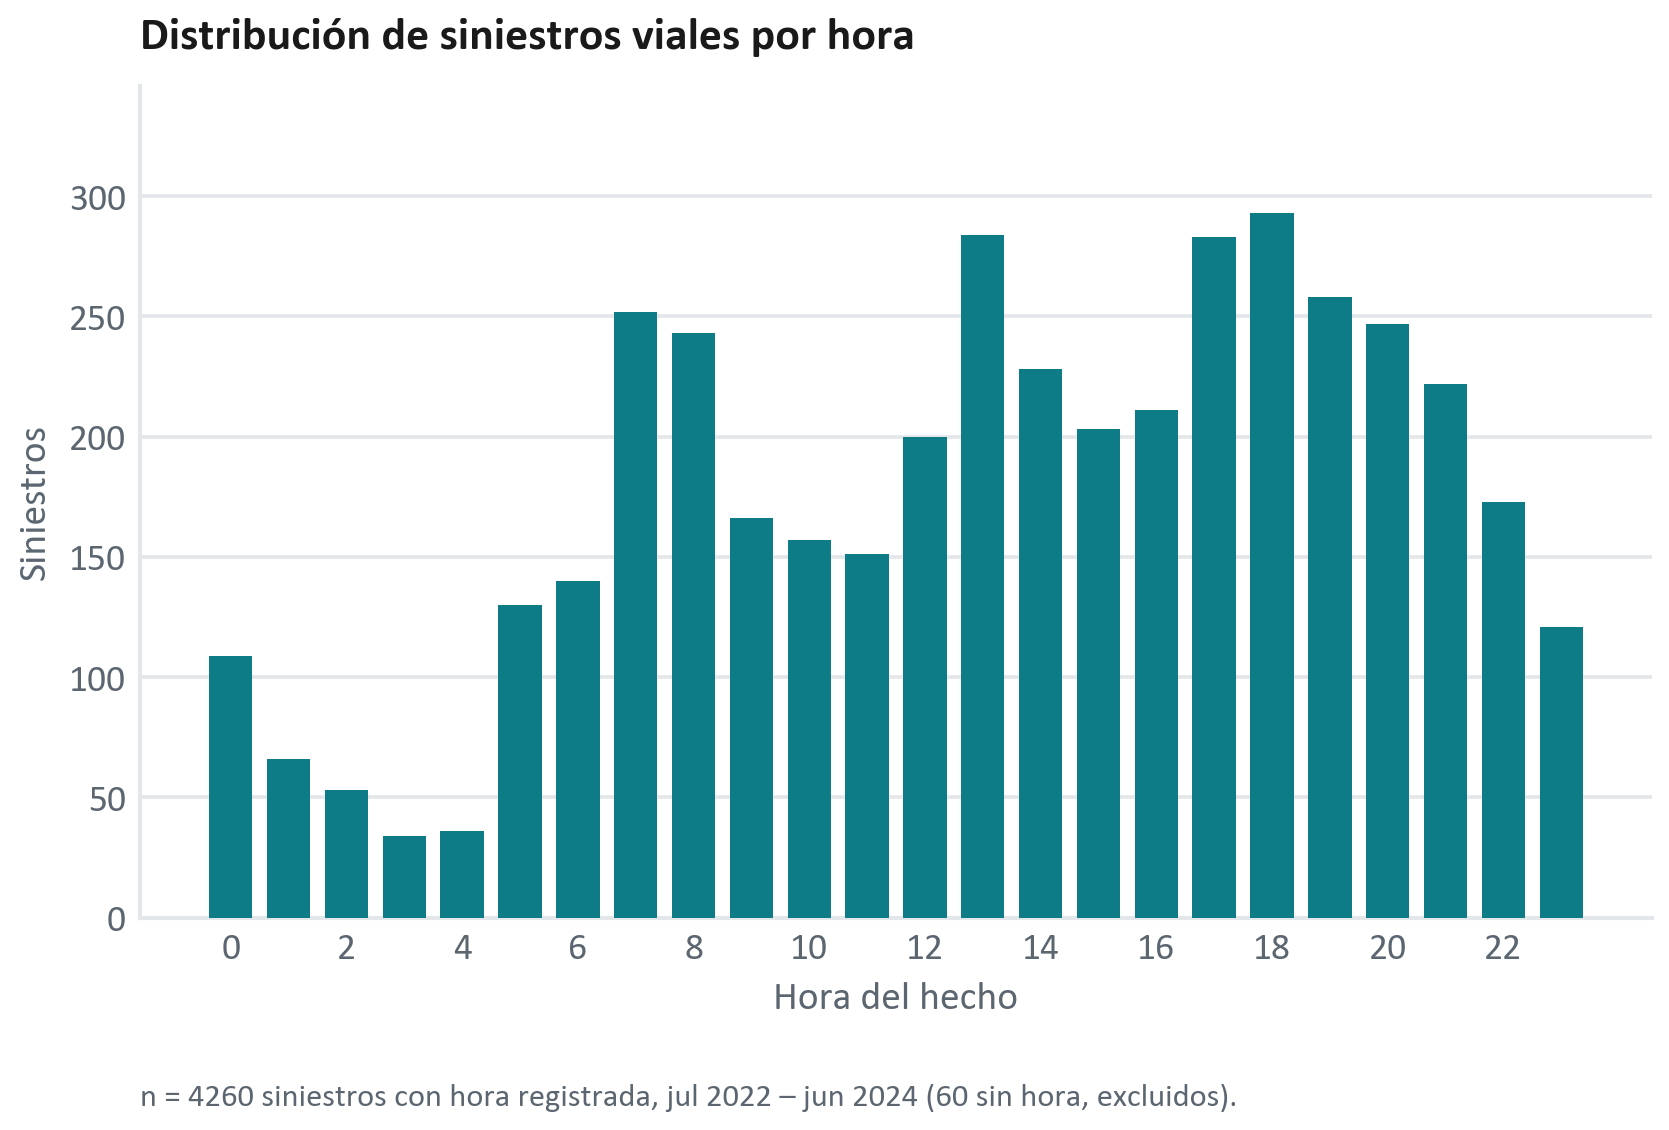
\includegraphics[width=0.85\linewidth]{imagenes/anexo_a2_distribucion_hora.png}
\caption{Distribución de siniestros viales por hora del hecho}
\label{fig:anexo-distribucion-hora}
\notaflot{Frecuencia horaria de los siniestros con hora registrada (n = 4260; 60 casos
sin dato, excluidos), julio 2022 -- junio 2024. Se identifican dos picos, uno hacia el
mediodía (13 h) y otro más pronunciado al final de la tarde (18 h), coincidentes con
los horarios de mayor circulación, y un mínimo en la madrugada (3--4 h). \fuentepropia{}.}
\end{figure}

\begin{figure}[htbp]
\centering
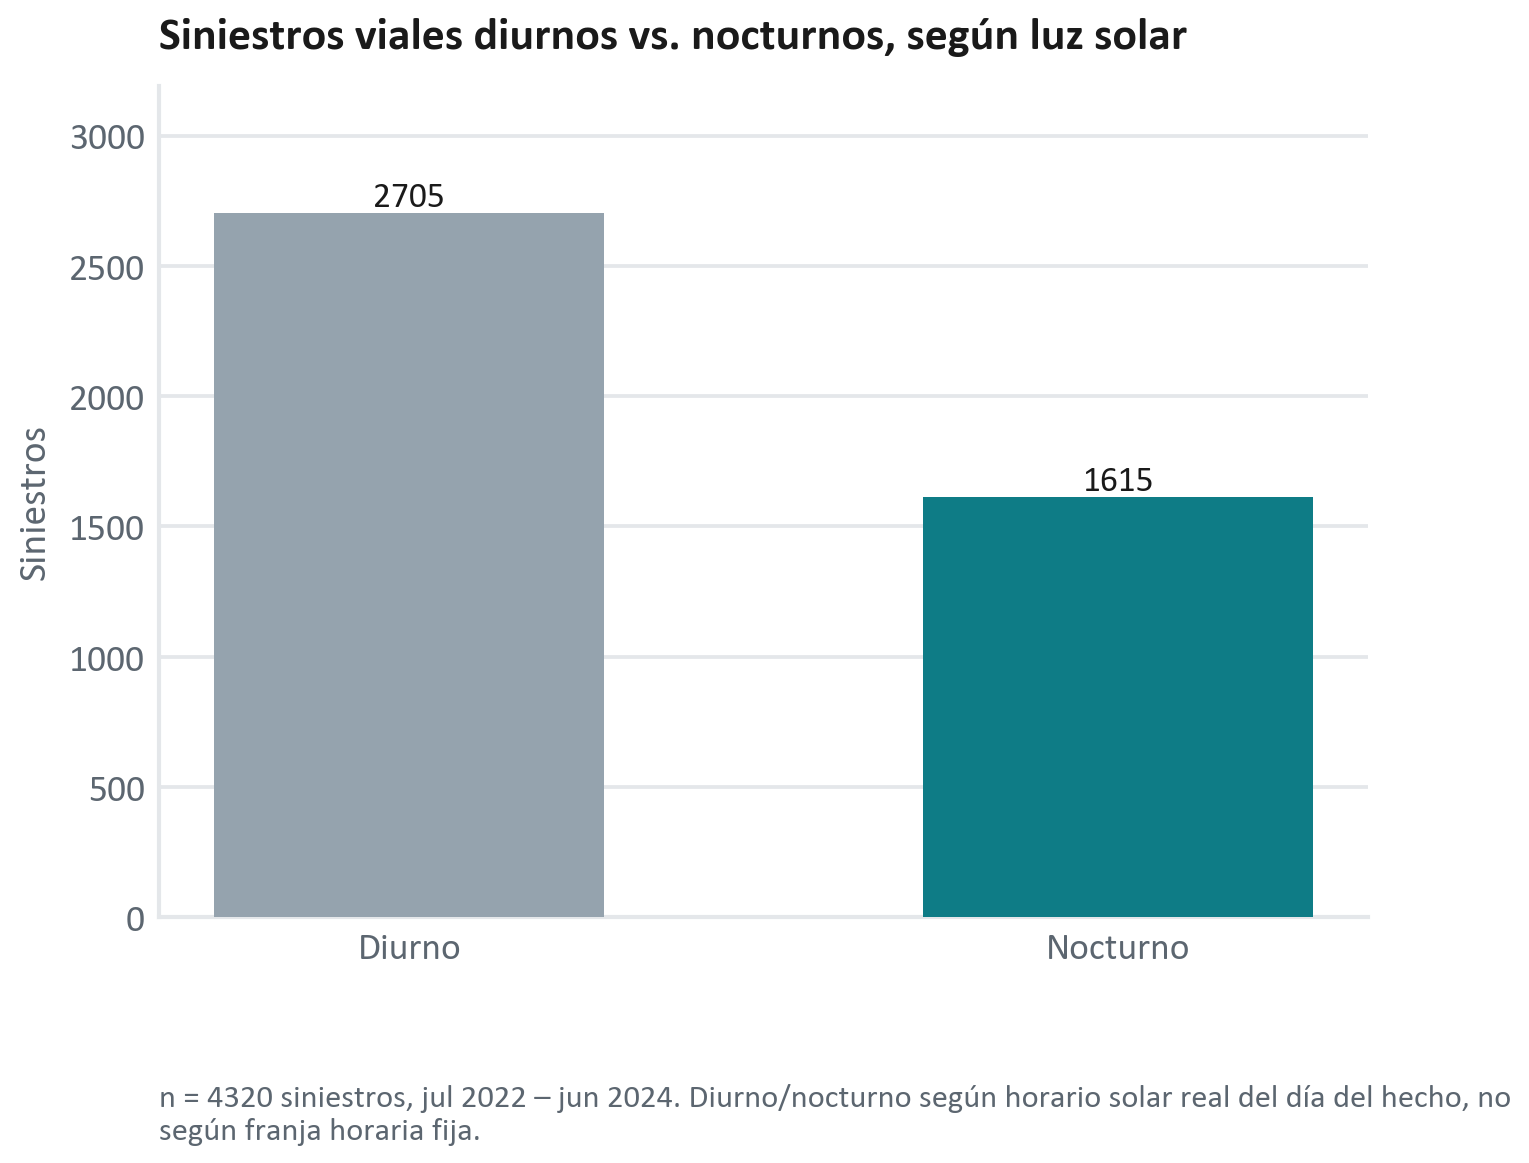
\includegraphics[width=0.7\linewidth]{imagenes/anexo_a2_diurno_nocturno.png}
\caption{Siniestros viales diurnos frente a nocturnos, según luz solar}
\label{fig:anexo-diurno-nocturno}
\notaflot{Clasificación de los 4320 siniestros según el horario solar real del día en
que ocurrieron, y no según una franja horaria fija. Un 63\,\% de los casos (2705)
ocurre en horario diurno y el 37\,\% restante (1615) en horario nocturno. \fuentepropia{}.}
\end{figure}

\begin{figure}[htbp]
\centering
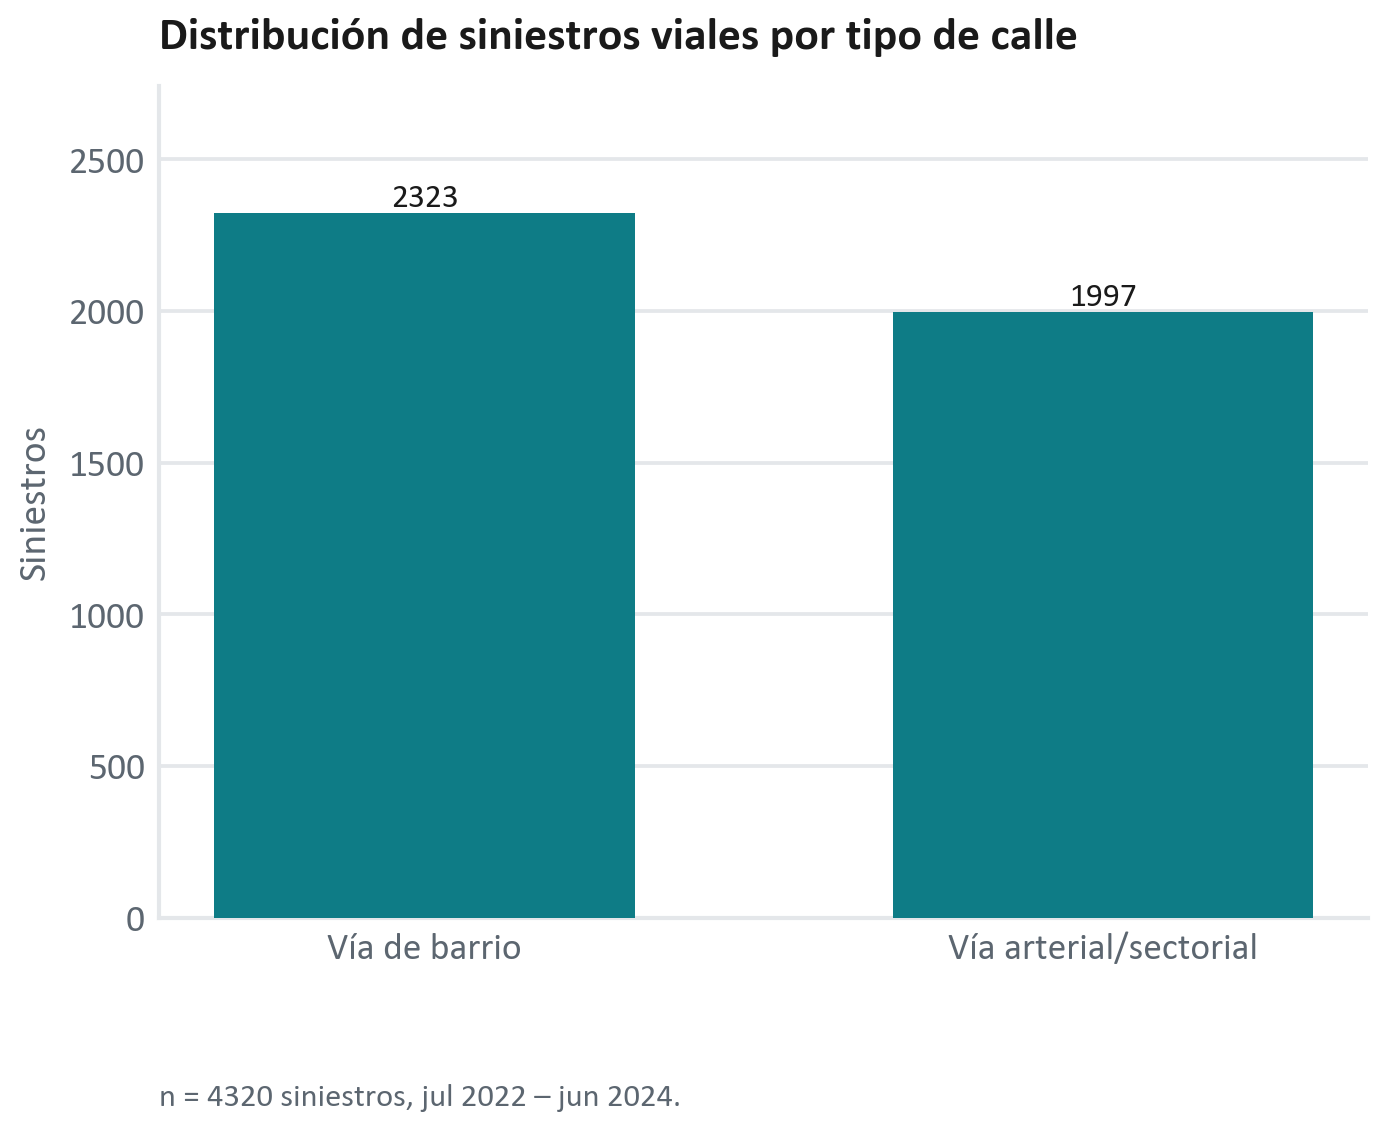
\includegraphics[width=0.78\linewidth]{imagenes/anexo_a2_tipo_calle.png}
\caption{Distribución de siniestros viales por tipo de calle}
\label{fig:anexo-tipo-calle}
\notaflot{Clasificación según jerarquía vial (n = 4320). Las vías de barrio concentran
algo más de la mitad de los casos (2323) frente a las vías arteriales o sectoriales
(1997), lo que confirma que el fenómeno no se limita a los corredores principales.
\fuentepropia{}.}
\end{figure}

\begin{figure}[htbp]
\centering
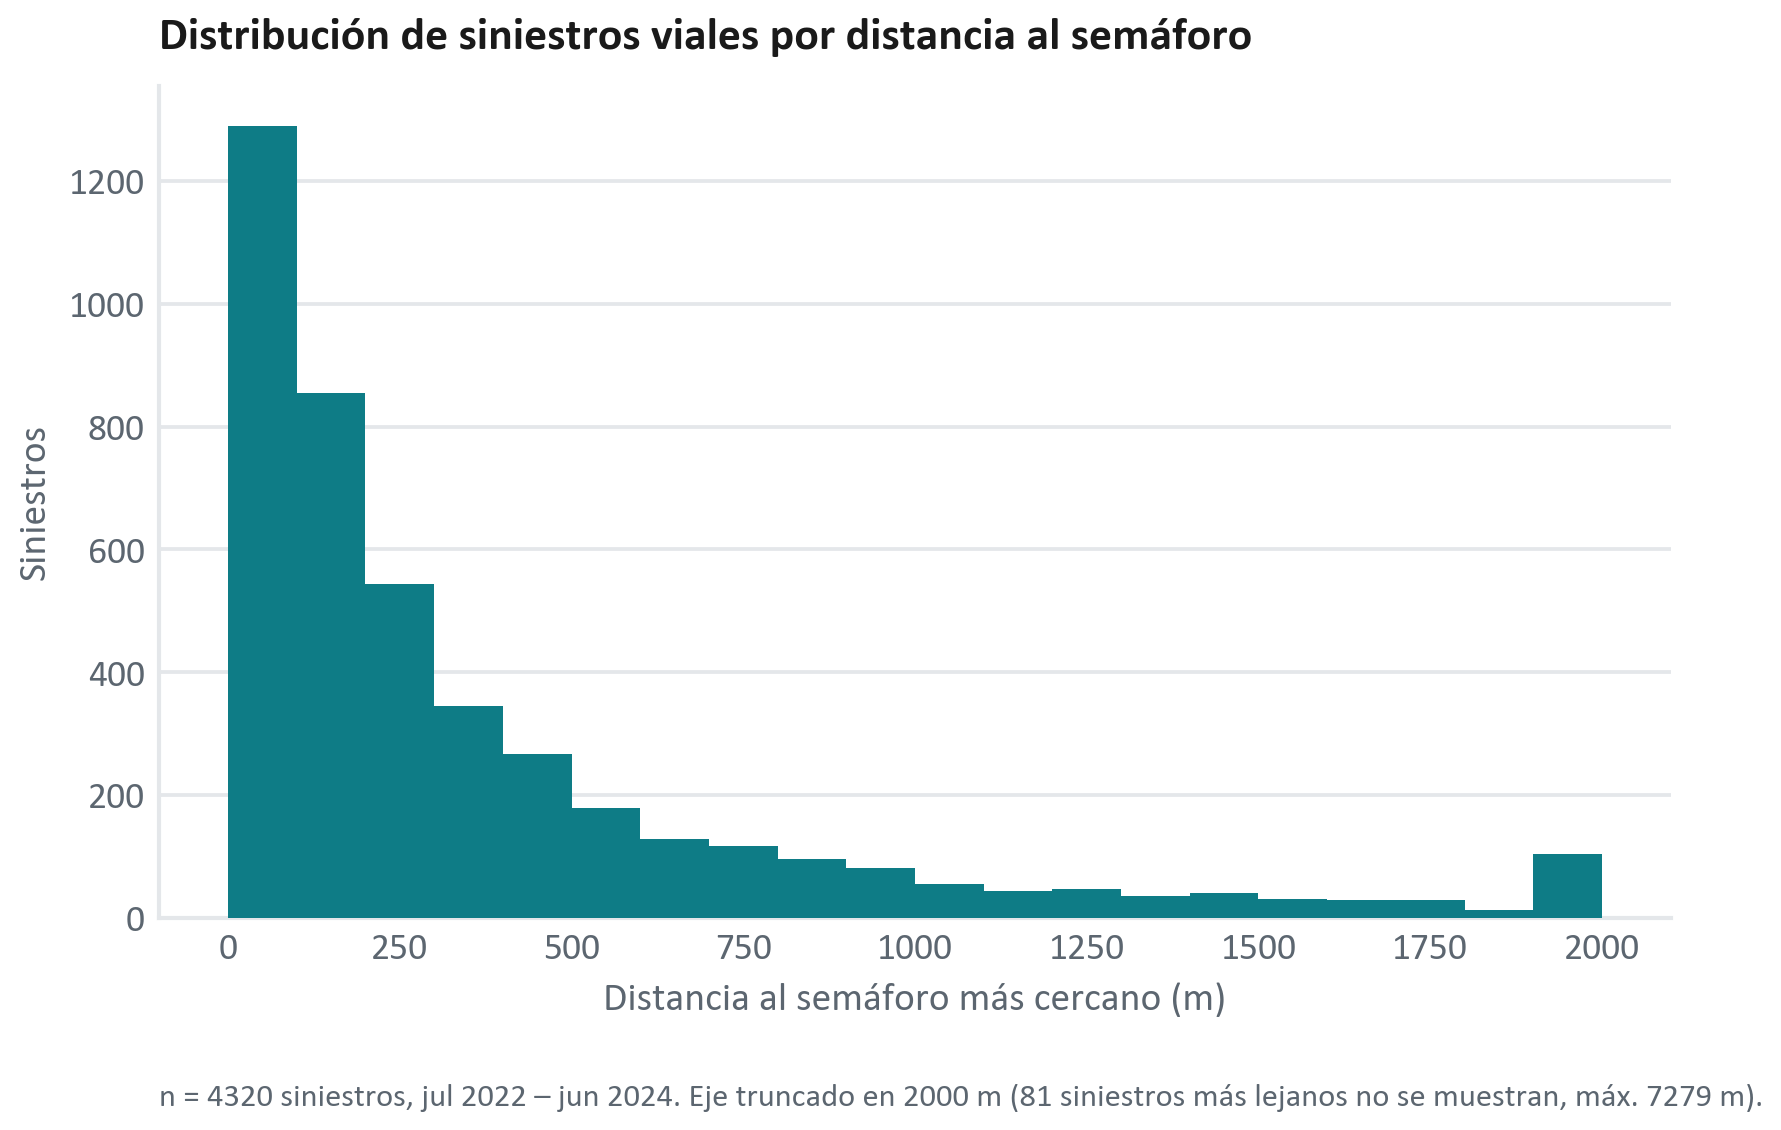
\includegraphics[width=0.8\linewidth]{imagenes/anexo_a2_distancia_semaforo.png}
\caption{Distribución de siniestros viales por distancia al semáforo más cercano}
\label{fig:anexo-distancia-semaforo}
\notaflot{Histograma de la distancia radial de cada siniestro al semáforo más cercano
(n = 4320; eje truncado en 2000 m, lo que deja fuera 81 casos más lejanos, con un
máximo de 7279 m). La frecuencia decrece marcadamente con la distancia: casi un
tercio de los siniestros ocurre a menos de 100 m de un semáforo. \fuentepropia{}.}
\end{figure}

\begin{figure}[htbp]
\centering
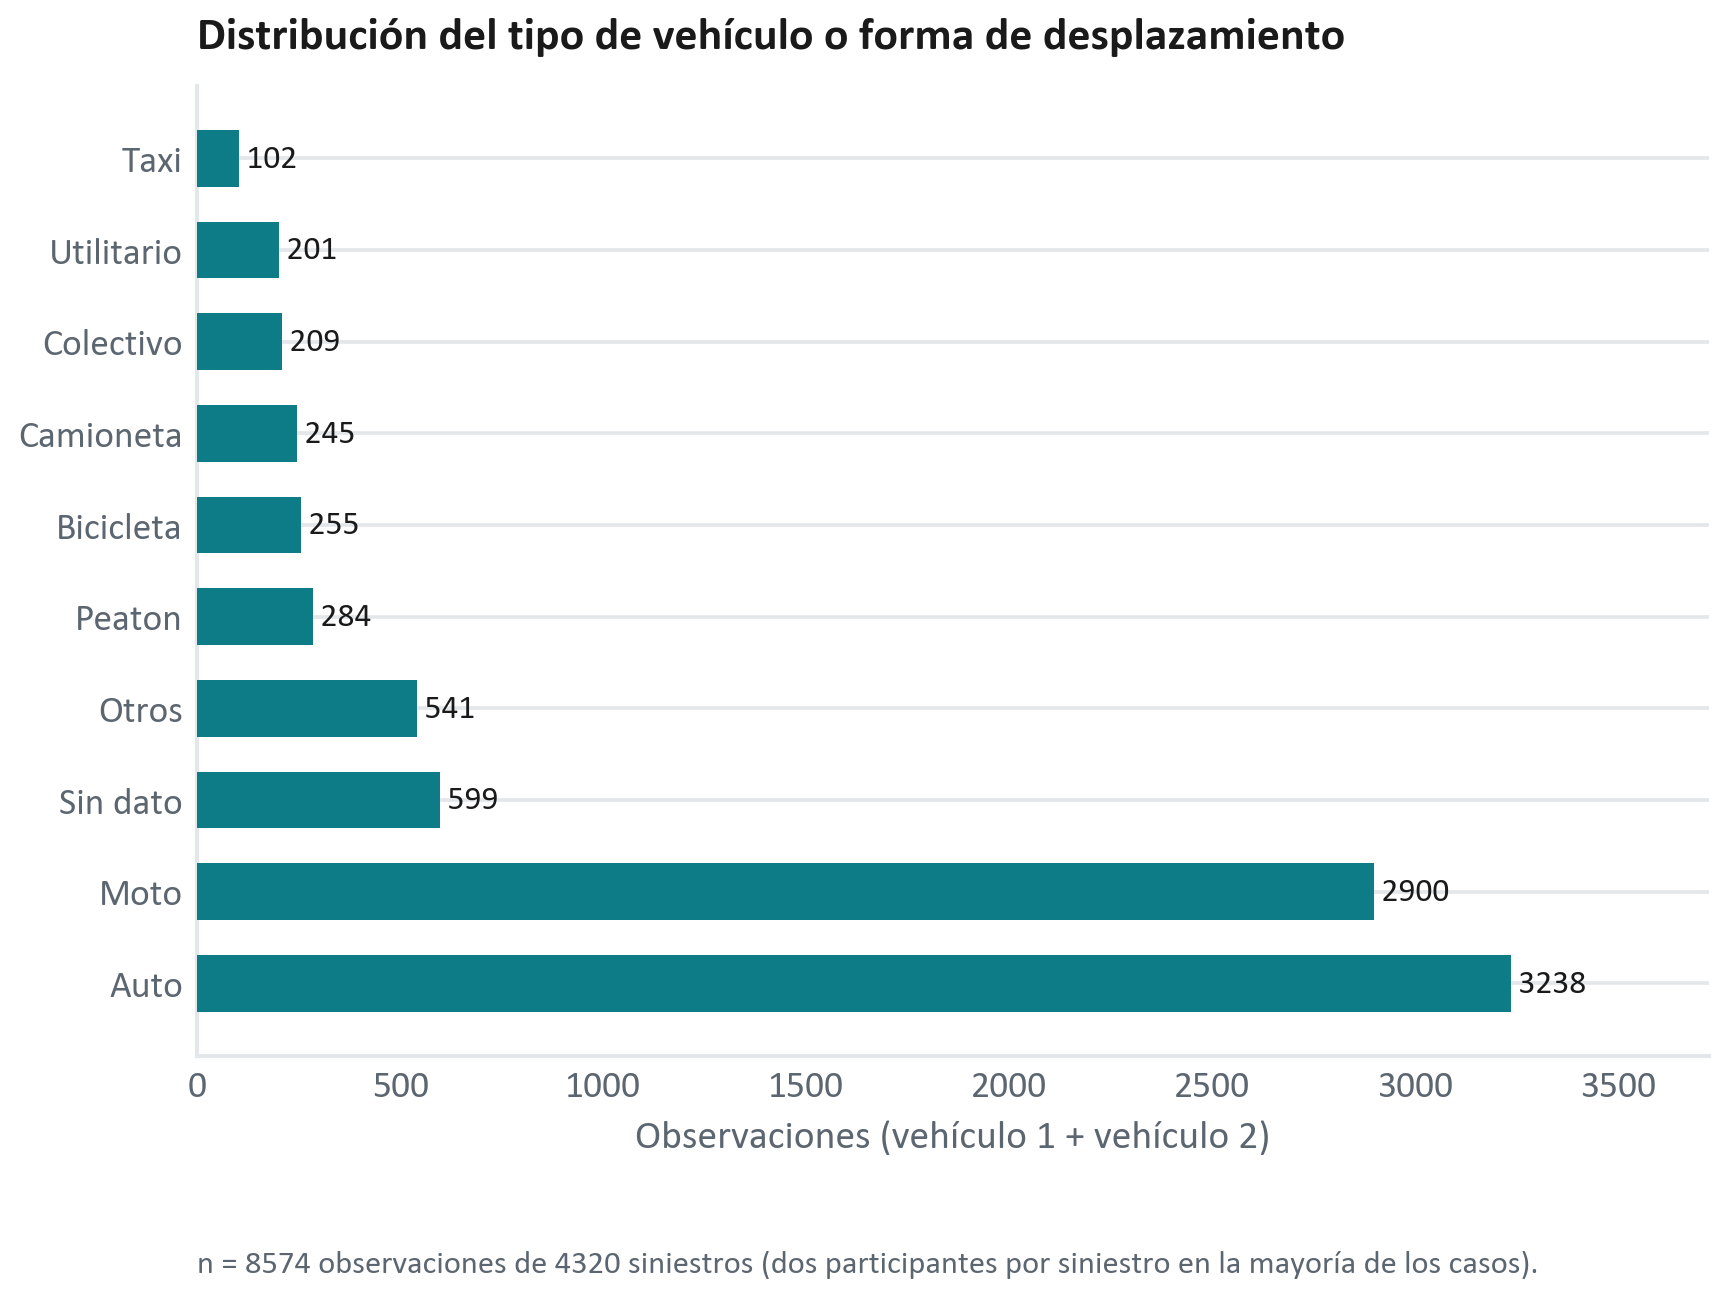
\includegraphics[width=0.8\linewidth]{imagenes/anexo_a2_tipo_vehiculo.png}
\caption{Distribución del tipo de vehículo o forma de desplazamiento}
\label{fig:anexo-tipo-vehiculo}
\notaflot{Participaciones registradas en los 4320 siniestros (n = 8574 observaciones,
correspondientes a vehículo 1 y vehículo 2 cuando corresponde). La unidad de conteo es
la participación y no el siniestro, por lo que las categorías no son excluyentes entre
sí. Los automóviles (3238) y las motocicletas (2900) concentran la mayor parte de las
observaciones. \fuentepropia{}.}
\end{figure}

\begin{figure}[htbp]
\centering
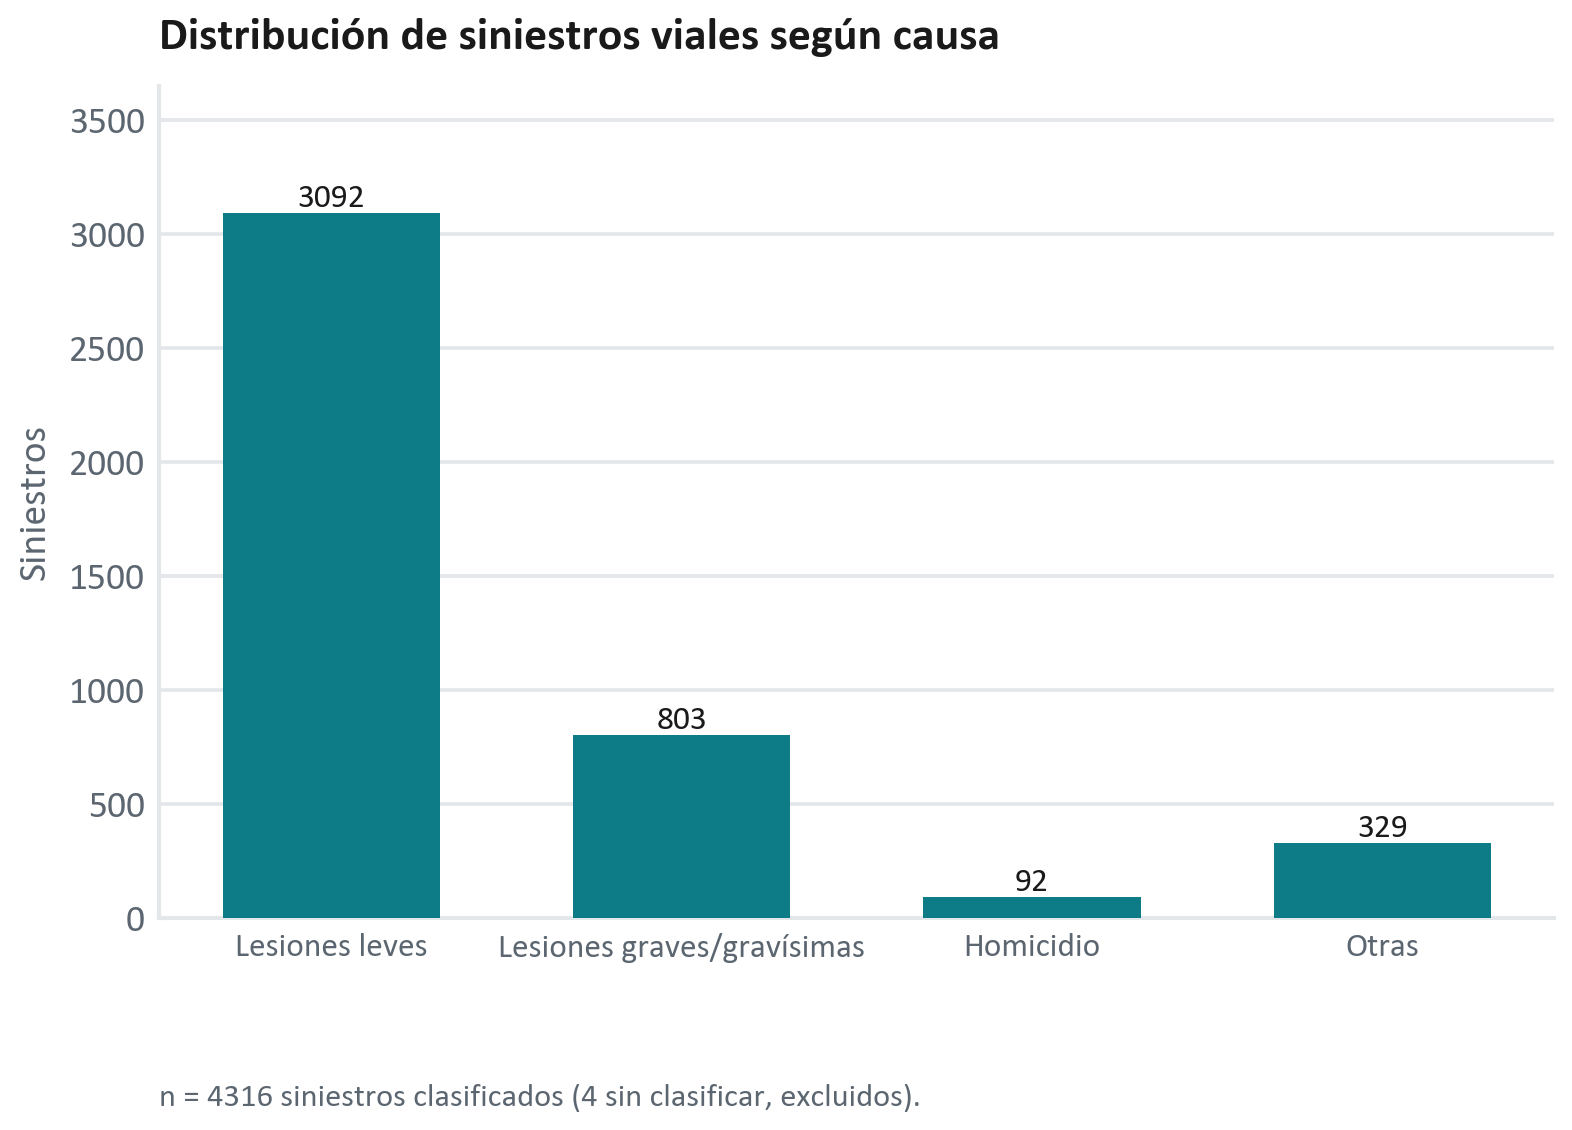
\includegraphics[width=0.75\linewidth]{imagenes/anexo_a2_causa.png}
\caption{Distribución de siniestros viales según causa}
\label{fig:anexo-causa}
\notaflot{Clasificación según la carátula asignada en la causa judicial (n = 4316; 4
casos sin clasificar, excluidos). Predominan las lesiones leves (3092), seguidas por
las lesiones graves o gravísimas (803), otras carátulas (329) y el homicidio culposo
(92). \fuentepropia{}.}
\end{figure}

\begin{figure}[htbp]
\centering
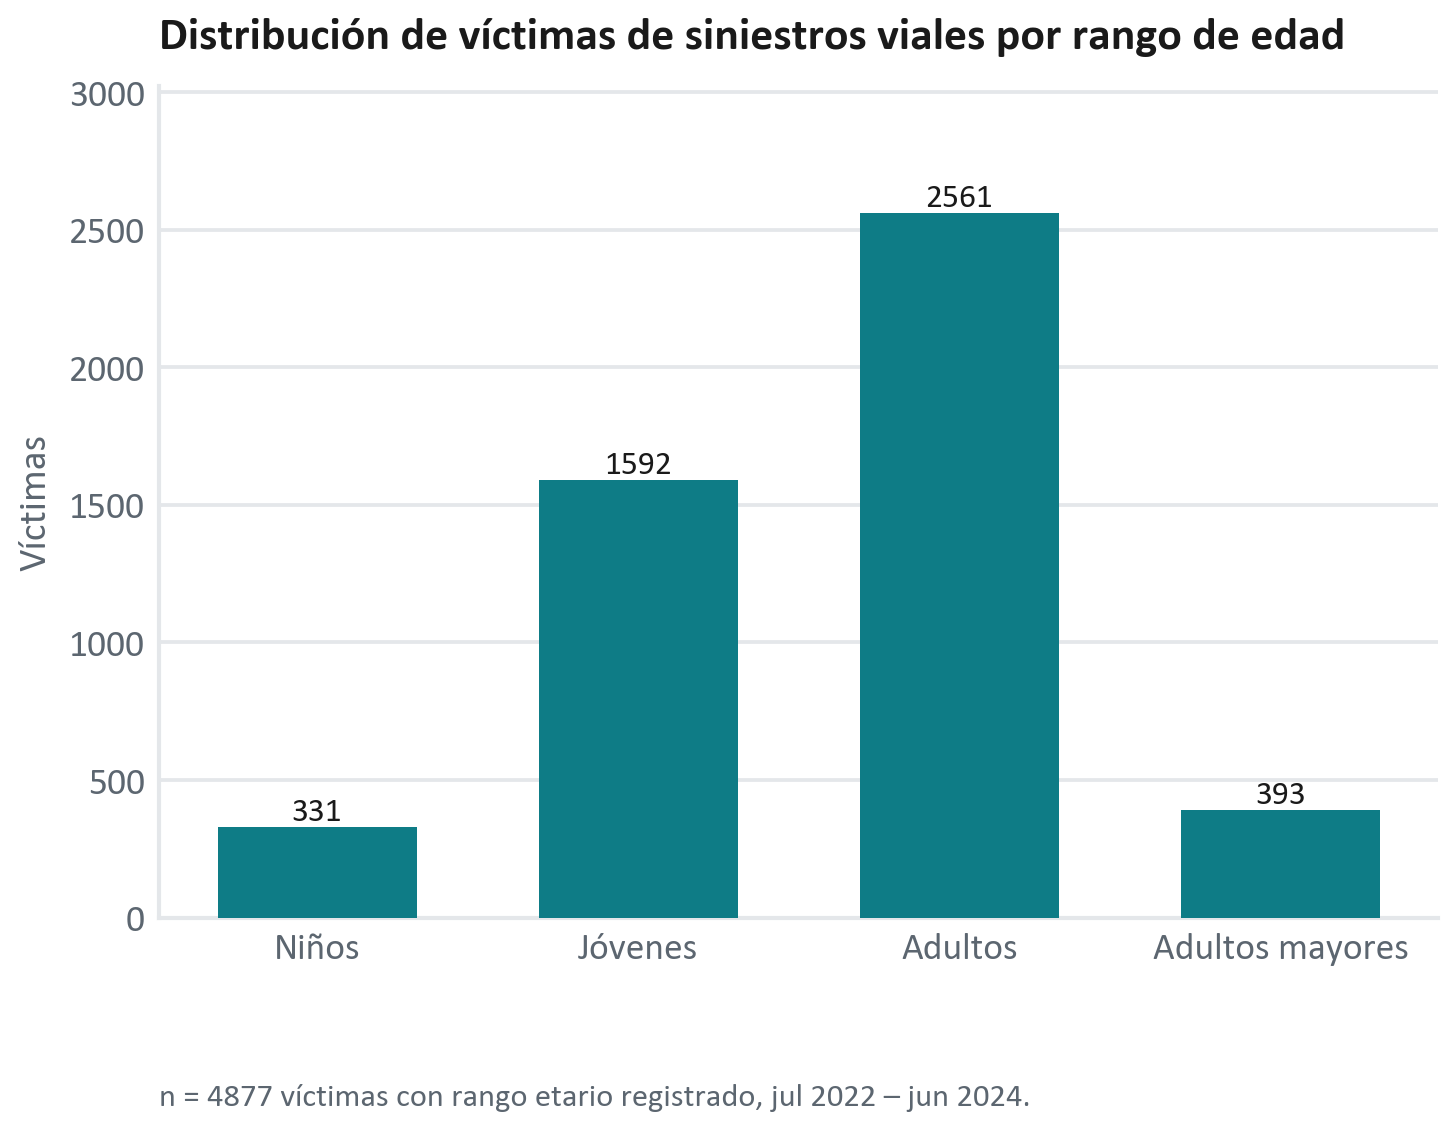
\includegraphics[width=0.75\linewidth]{imagenes/anexo_a2_rango_edad.png}
\caption{Distribución de víctimas de siniestros viales por rango etario}
\label{fig:anexo-rango-edad}
\notaflot{Distribución etaria de las víctimas con dato de edad registrado (n = 4877),
según los rangos definidos por la Organización Mundial de la Salud. Los adultos (27 a
59 años) concentran la mayor cantidad de víctimas (2561), seguidos por los jóvenes de
15 a 26 años (1592). \fuentepropia{}.}
\end{figure}

\begin{figure}[htbp]
\centering
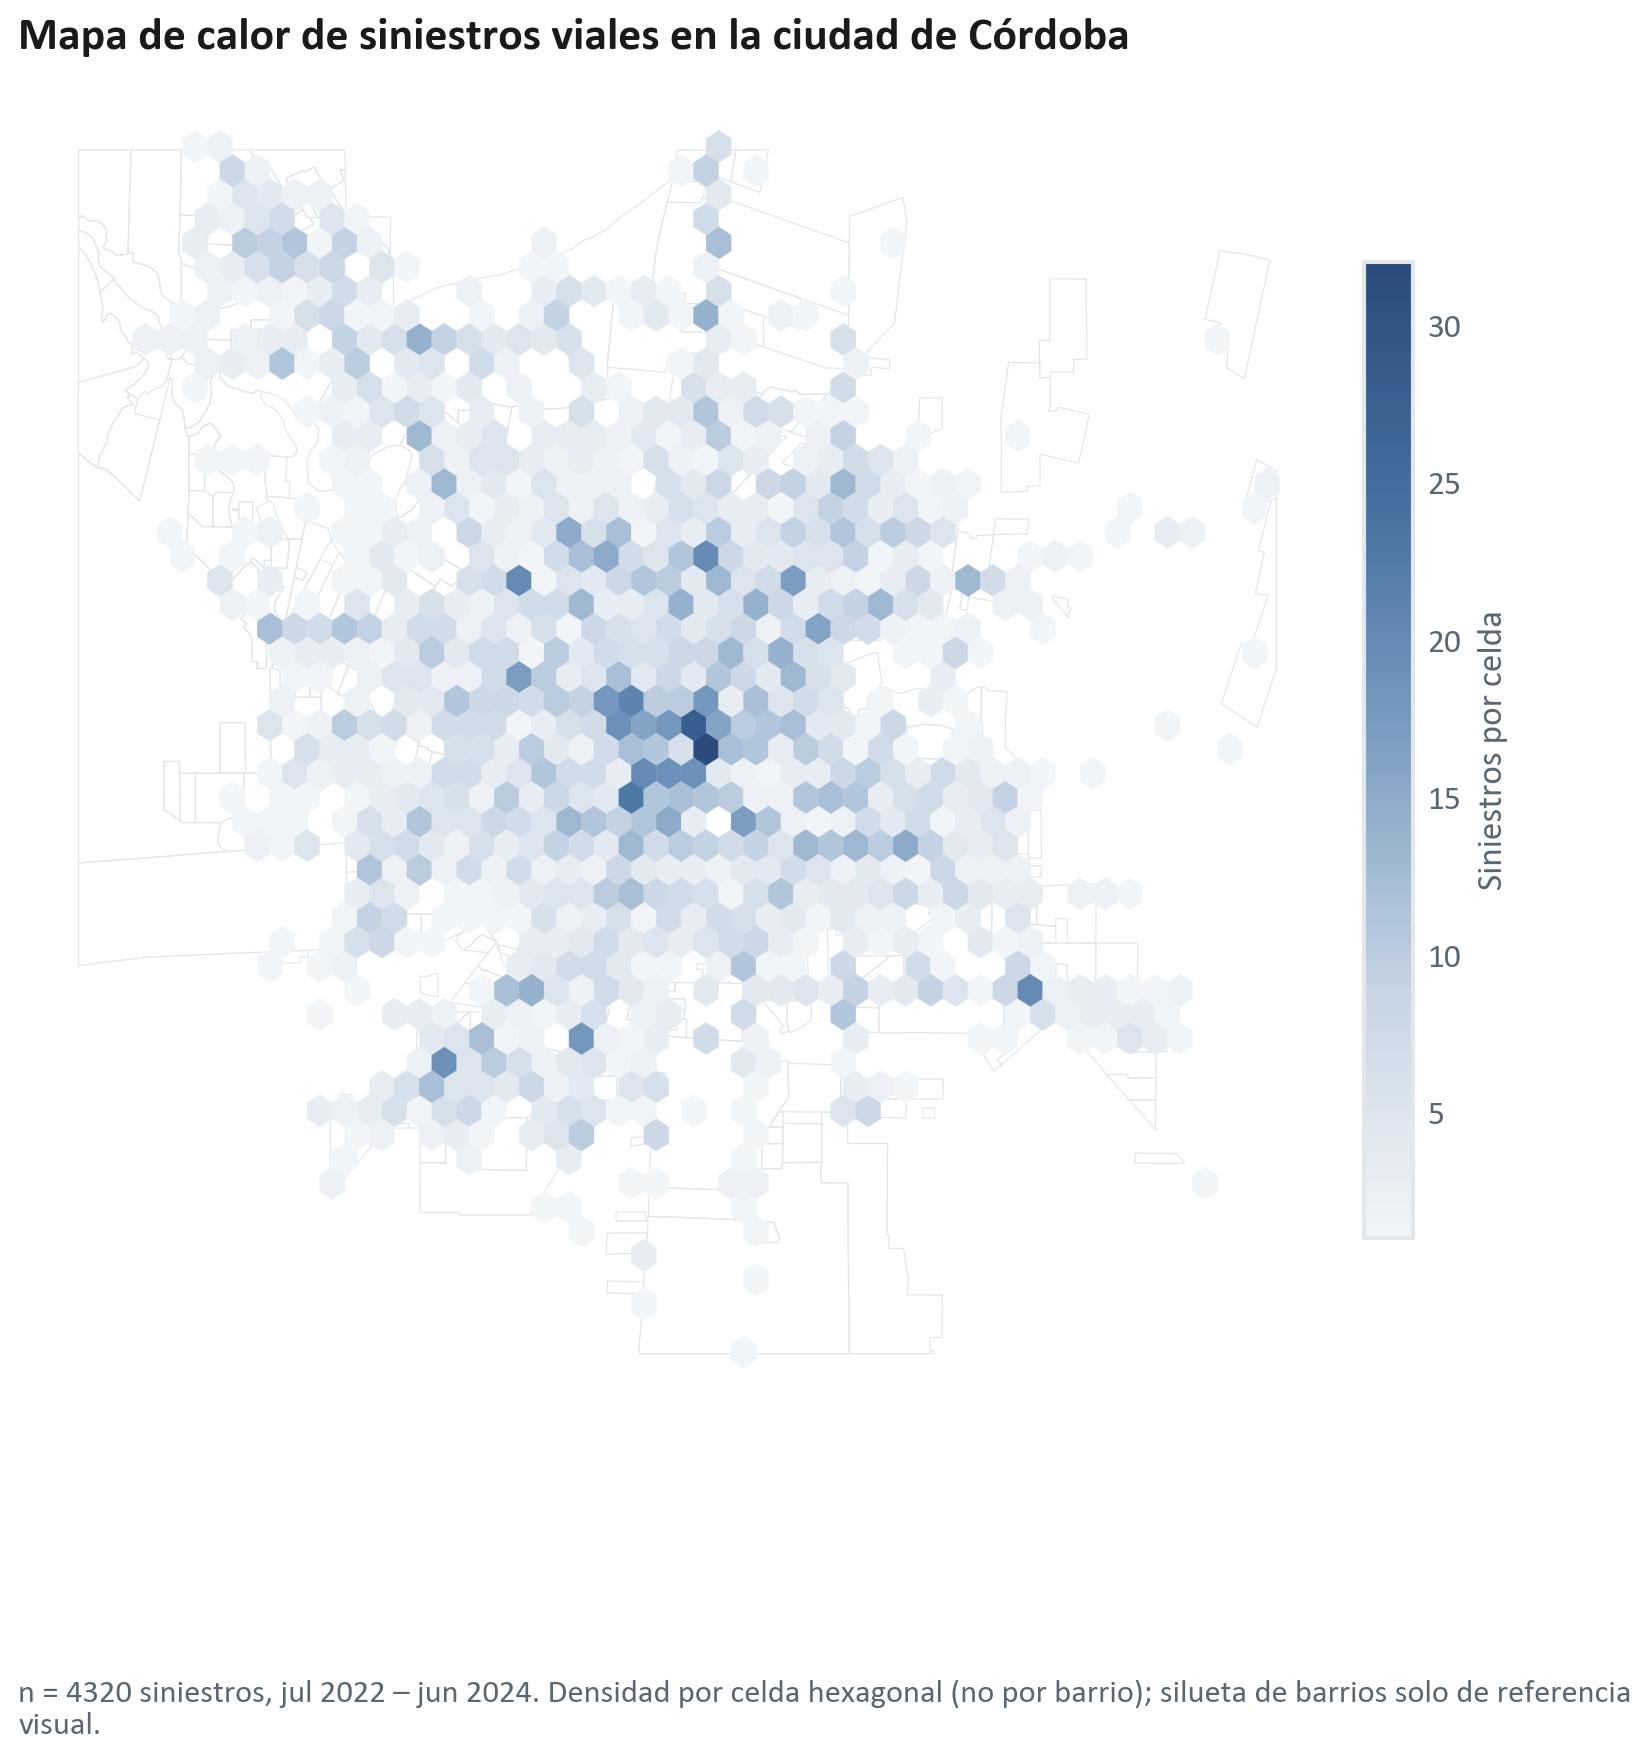
\includegraphics[width=0.62\linewidth]{imagenes/anexo_a2_mapa_calor_ciudad.png}
\caption{Mapa de calor de siniestros viales en la ciudad de Córdoba}
\label{fig:anexo-mapa-calor-ciudad}
\notaflot{Densidad espacial de los 4320 siniestros georreferenciados, agregada por
celda hexagonal de superficie constante; la silueta de barrios se incluye solo como
referencia visual. Se observa una concentración marcada en el área central, con
máximos puntuales superiores a 30 siniestros por celda. \fuentepropia{}.}
\end{figure}

\begin{figure}[htbp]
\centering
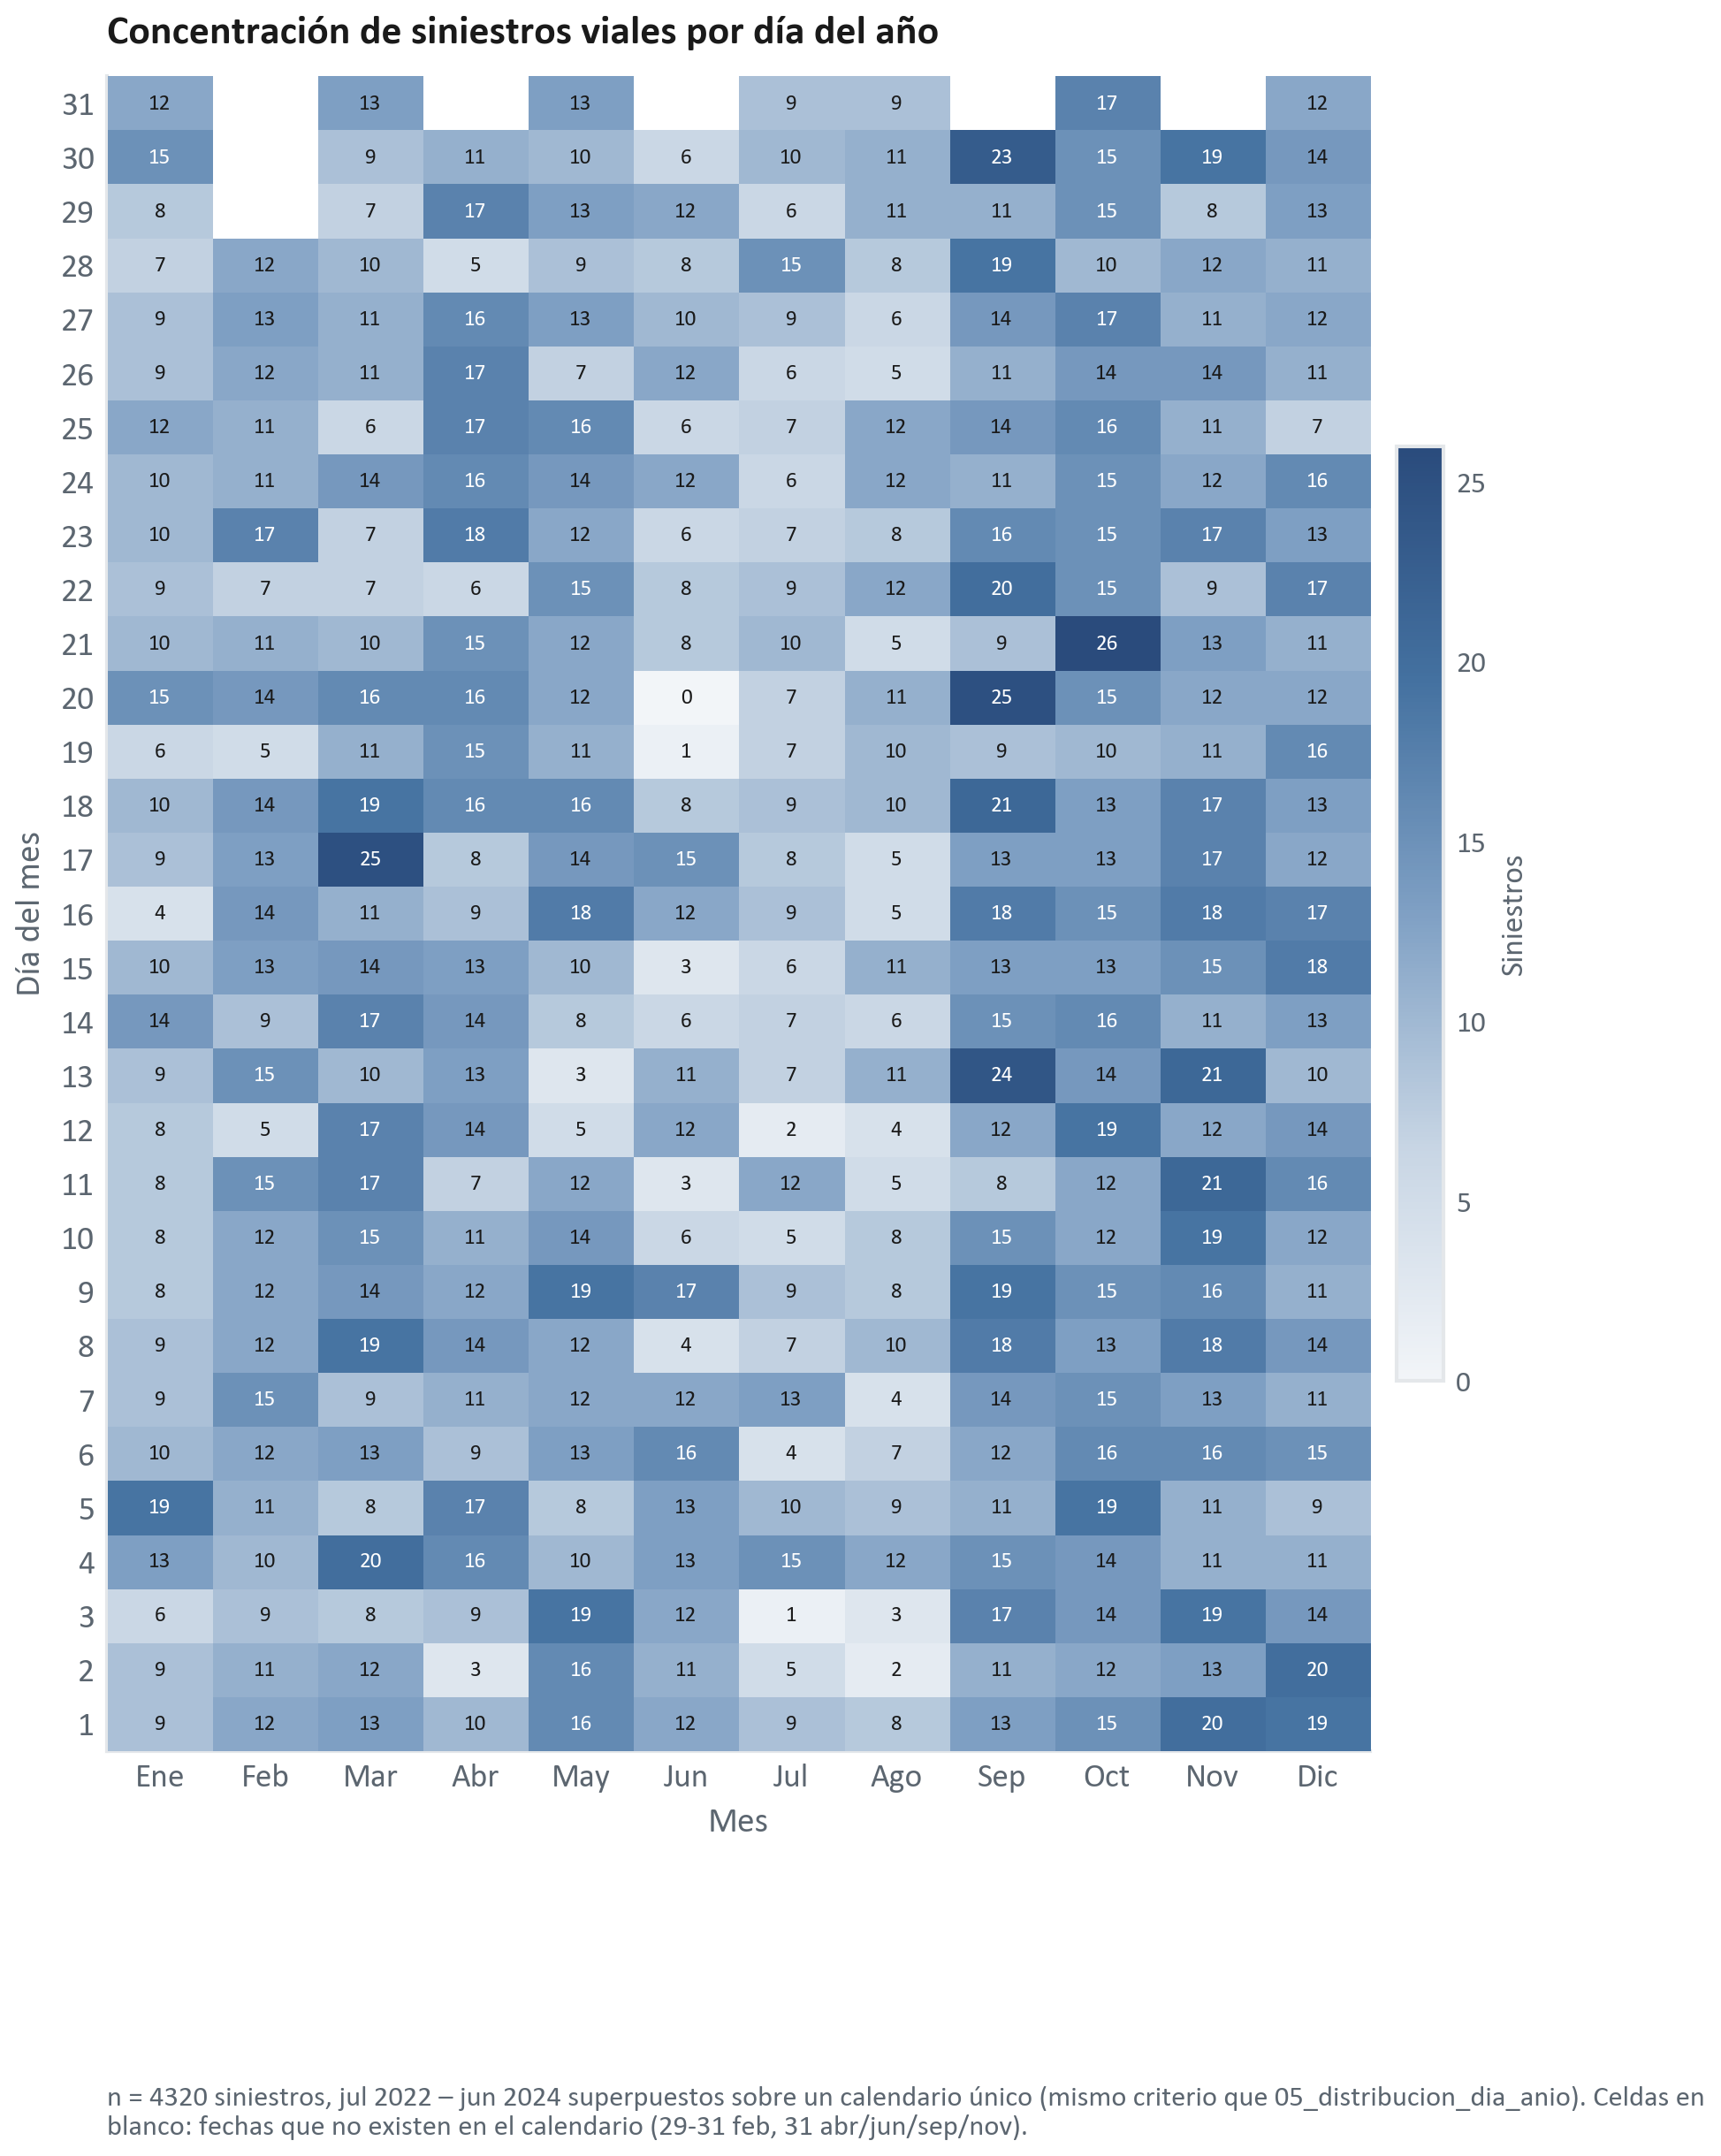
\includegraphics[width=0.7\linewidth]{imagenes/anexo_a2_mapa_calor_dia_anio.png}
\caption{Concentración de siniestros viales por día del año}
\label{fig:anexo-mapa-calor-dia-anio}
\notaflot{Representación matricial (mes por día del mes) de la misma distribución
diaria presentada en la \cref{fig:anexo-distribucion-dia-anio} (n = 4320, mismo
criterio de superposición sobre un calendario único). Las celdas en blanco
corresponden a fechas que no existen en el calendario (29 a 31 de febrero, y el día 31
de abril, junio, septiembre y noviembre). \fuentepropia{}.}
\end{figure}

%% =====================================================================
%% 11. LISTADO DE SÍMBOLOS Y CONVENCIONES
%% =====================================================================

\chapter{Listado de símbolos y convenciones}\label{listado-de-simbolos-y-convenciones}

Este apéndice reúne las siglas, los símbolos matemáticos y las convenciones de
notación empleadas a lo largo del documento. Su finalidad es que cualquier
lector pueda interpretar sin ambigüedad las tablas, ecuaciones y métricas
presentadas en los capítulos anteriores.

\section*{Siglas y acrónimos}
\addcontentsline{toc}{section}{Siglas y acrónimos}

\begin{longtable}[]{@{}ll@{}}
\toprule
\textbf{Sigla} & \textbf{Significado} \\
\midrule
\endfirsthead
\toprule
\textbf{Sigla} & \textbf{Significado} \\
\midrule
\endhead
\bottomrule
\endlastfoot
API & \eng{Application Programming Interface} \\
ARIMA & \eng{AutoRegressive Integrated Moving Average} \\
AUC & \eng{Area Under the Curve} \\
CatBoost & \eng{Categorical Boosting} \\
CCAD & Centro de Computación de Alto Desempeño (UNC) \\
CPU & \eng{Central Processing Unit} \\
DeepAR & \eng{Deep AutoRegressive} \\
EFB & \eng{Exclusive Feature Bundling} \\
ERIA & Ética, Regulaciones e Impacto de la IA (área de LIDeSIA) \\
ETS & \eng{Error, Trend, Seasonality} \\
FCEFyN & Facultad de Ciencias Exactas, Físicas y Naturales \\
GBM & \eng{Gradient Boosting Machine} \\
GNN & \eng{Graph Neural Network} \\
GOSS & \eng{Gradient-based One-Side Sampling} \\
GPU & \eng{Graphics Processing Unit} \\
IA & Inteligencia artificial \\
IEC & \eng{International Electrotechnical Commission} \\
ISO & \eng{International Organization for Standardization} \\
ITID & Infraestructura Tecnológica e Ingeniería de Datos (área de LIDeSIA) \\
LIDeSIA & Laboratorio de Investigación y Desarrollo de Software e IA \\
LightGBM & \eng{Light Gradient Boosting Machine} \\
LLM & \eng{Large Language Model} \\
LSTM & \eng{Long Short-Term Memory} \\
MAE & \eng{Mean Absolute Error} \\
MASE & \eng{Mean Absolute Scaled Error} \\
MIA & Matemática para la IA (área de LIDeSIA) \\
ML & \eng{Machine Learning} (aprendizaje automático) \\
MLP & \eng{Multilayer Perceptron} (perceptrón multicapa) \\
MPF & Ministerio Público Fiscal de la Provincia de Córdoba \\
MSE & \eng{Mean Squared Error} \\
MVP & \eng{Minimum Viable Product} (producto mínimo viable) \\
PatchTST & \eng{Patch Time Series Transformer} \\
PMI & \eng{Project Management Institute} \\
PPT & Personas, procesos y tecnología \\
PR-AUC & \eng{Precision-Recall Area Under the Curve} \\
RAG & \eng{Red, Amber, Green} (codificación de alertas por color) \\
RAM & \eng{Random Access Memory} \\
RMSE & \eng{Root Mean Squared Error} \\
ROC & \eng{Receiver Operating Characteristic} \\
SAC & Sistema de Administración de Causas \\
SAT & Sistema de alerta temprana \\
SGAV & Sistema de Gestión de Siniestros Viales \\
SLURM & \eng{Simple Linux Utility for Resource Management} \\
TFT & \eng{Temporal Fusion Transformer} \\
TRL & \eng{Technology Readiness Level} (nivel de madurez tecnológica) \\
UJ & Unidad Judicial \\
UNC & Universidad Nacional de Córdoba \\
XAI & \eng{Explainable Artificial Intelligence} (IA explicable) \\
XGBoost & \eng{Extreme Gradient Boosting} \\
\end{longtable}

\section*{Símbolos matemáticos}
\addcontentsline{toc}{section}{Símbolos matemáticos}

\begin{longtable}[]{@{}>{$}l<{$}p{10.5cm}@{}}
\toprule
\multicolumn{1}{@{}l}{\textbf{Símbolo}} & \textbf{Significado} \\
\midrule
\endfirsthead
\toprule
\multicolumn{1}{@{}l}{\textbf{Símbolo}} & \textbf{Significado} \\
\midrule
\endhead
\bottomrule
\endlastfoot
K & Cantidad de variables medidas simultáneamente en el sistema multivariado. \\
T & Cantidad total de instantes de tiempo de la serie. \\
t & Índice del paso de tiempo (bloque de seis horas). \\
\mathbf{z}_t & Vector de observaciones en el instante $t$, con $\mathbf{z}_t \in \mathbb{R}^{K}$. \\
\mathbf{Z} & Matriz de datos original, de dimensiones $T \times K$. \\
n & Cantidad de observaciones del conjunto de entrenamiento. \\
N & Cantidad de muestras del conjunto de prueba. \\
y_i & Valor observado de la variable objetivo para la observación $i$. \\
\hat{y}_i & Valor predicho por el modelo para la observación $i$. \\
\hat{y}^{(t-1)}_i & Predicción acumulada tras $t-1$ iteraciones de \eng{boosting}. \\
f_t & Árbol incorporado en la iteración $t$ del \eng{boosting}. \\
\mathcal{L}^{(t)} & Función objetivo de XGBoost en la iteración $t$. \\
\Omega(f_t) & Término de regularización que penaliza la complejidad del árbol. \\
g_i & Gradiente de primer orden de la función de pérdida. \\
h_i & Gradiente de segundo orden (hessiano) de la función de pérdida. \\
M & Cantidad de modelos que participan del ensamble ponderado. \\
w_m & Peso asignado al modelo $m$ en el ensamble, con $\sum w_m = 1$ y $w_m \geq 0$. \\
m & Período estacional de la serie ($m = 4$ bloques por día). \\
z & Puntaje estándar (\eng{Z-Score}) usado por la capa de decisión. \\
\sigma & Desviación estándar del comportamiento histórico. \\
\text{P10},\ \text{P90} & Cuantiles 10\,\% y 90\,\% del intervalo de predicción. \\
\end{longtable}

\section*{Convenciones de notación}
\addcontentsline{toc}{section}{Convenciones de notación}

\begin{description}
  \item[Separadores numéricos.] Se emplea la coma como separador decimal y el
    punto como separador de miles a partir de cinco cifras, según la convención
    del español rioplatense. Los valores tomados de salidas de software fueron
    convertidos a esta notación.
  \item[Nombres de variables.] Los campos del conjunto de datos y los
    hiperparámetros de los modelos se escriben en tipografía monoespaciada,
    respetando la grafía exacta con la que figuran en el código:
    \var{TARGET\_CRITICO}, \var{promedio\_victimas\_24h}, \var{max\_depth}.
  \item[Términos en inglés.] Los anglicismos técnicos sin traducción consolidada
    se escriben en cursiva (\eng{forecasting}, \eng{baseline}, \eng{recall}).
    Cuando existe equivalente en español se usa este último, indicando el
    término original entre paréntesis en su primera aparición.
  \item[Nombres de modelos y librerías.] Se respeta la grafía oficial de cada
    proyecto: XGBoost, LightGBM, AutoGluon, AutoGluon-TimeSeries, CatBoost.
  \item[Tablas y figuras.] Los elementos tabulares se denominan \emph{tablas} y
    los gráficos, \emph{figuras}; ambos se numeran por capítulo y se referencian
    de forma cruzada. Cada uno lleva al pie una nota en formato APA que indica
    su alcance y su fuente.
  \item[Niveles de alerta.] La codificación por color sigue el criterio definido
    en la sección de tipos de alerta: verde (línea de base), amarillo
    (prevención), naranja (alerta) y rojo (crítico).
  \item[Bloques temporales.] Salvo indicación en contrario, la unidad de
    agregación es el bloque de seis horas; el bloque 1 abarca de 00:00 a 06:00 y
    los restantes se numeran de forma consecutiva.
\end{description}

\end{document}
